\documentclass[a4paper,oneside]{book}
% \documentclass[a4paper]{report}
\usepackage{a4wide}
\usepackage[english]{babel}
% Used for images
% \usepackage{subfig}
\usepackage{graphicx}
\graphicspath{{./img/}}
% Used for captions and subcaptions on images
\usepackage[labelfont=rm]{caption}
\usepackage{subcaption}
\usepackage{booktabs}
\usepackage{rotating} 
% Used for tables
\usepackage{tabu}
\usepackage{ragged2e}
\usepackage{caption, copyrightbox}
\usepackage[utf8]{inputenc}
\usepackage{array}
\usepackage{wrapfig}
\usepackage{multirow}
\usepackage{tabularx}
\usepackage{colortbl}
\usepackage[table]{xcolor}
\usepackage{pdfpages}
\usepackage[a4paper,includeheadfoot,margin=2.50cm]{geometry}
\usepackage{lipsum}
\usepackage{float}
\usepackage{amsmath}
\usepackage{multicol}
\usepackage{csquotes}
\usepackage{verbatim}
\usepackage{makecell}
\usepackage{gensymb}
\usepackage{dingbat}
\usepackage{siunitx}
\usepackage{afterpage}
\sisetup{detect-all}
\usepackage[acronym]{glossaries}
\setlength{\parskip}{1em}
\setlength{\parindent}{0.5em}
% References
\usepackage[
style=authoryear-comp,
maxnames=1,
minnames=1,
sorting=nyt,
uniquename=false,
uniquelist=minyear,
labeldateparts=true,
natbib,
url=false,
]{biblatex}
\addbibresource{references.bib}
\addbibresource{pieters_tables.bib}
\usepackage{hyperref}
\usepackage{fancyhdr}
\usepackage[clean]{svg}

% Footnotes
\usepackage[symbol]{footmisc}
\renewcommand{\thefootnote}{\fnsymbol{footnote}}

% custom fonts
\usepackage[T1]{fontenc}
\usepackage{palatino}

% print url if no doi
\renewbibmacro*{doi+eprint+url}{%
    \printfield{doi}%
    \newunit\newblock%
    \iftoggle{bbx:eprint}{%
        \usebibmacro{eprint}%
    }{}%
    \newunit\newblock%
    \iffieldundef{doi}{%
        \usebibmacro{url+urldate}}%
        {}%
    }

\makeglossaries

% toc spacing
\usepackage{tocloft}
\setlength\cftparskip{2pt}
% \setlength\cftbeforechapskip{12pt}


%%%% CONTENT %%%%


% zodat chapter titles niet midden op de pagina komen
\usepackage{titlesec}
\titleformat{\chapter}[display]   
{\normalfont\huge\bfseries}{\chaptertitlename\ \thechapter}{20pt}{\Huge}  
\titlespacing*{\chapter}{0pt}{-50pt}{40pt}

\def \myMargin {0.4cm}
\begin{document}
\pagenumbering{gobble}

% mandatory opening pages
\afterpage{\null\newpage}
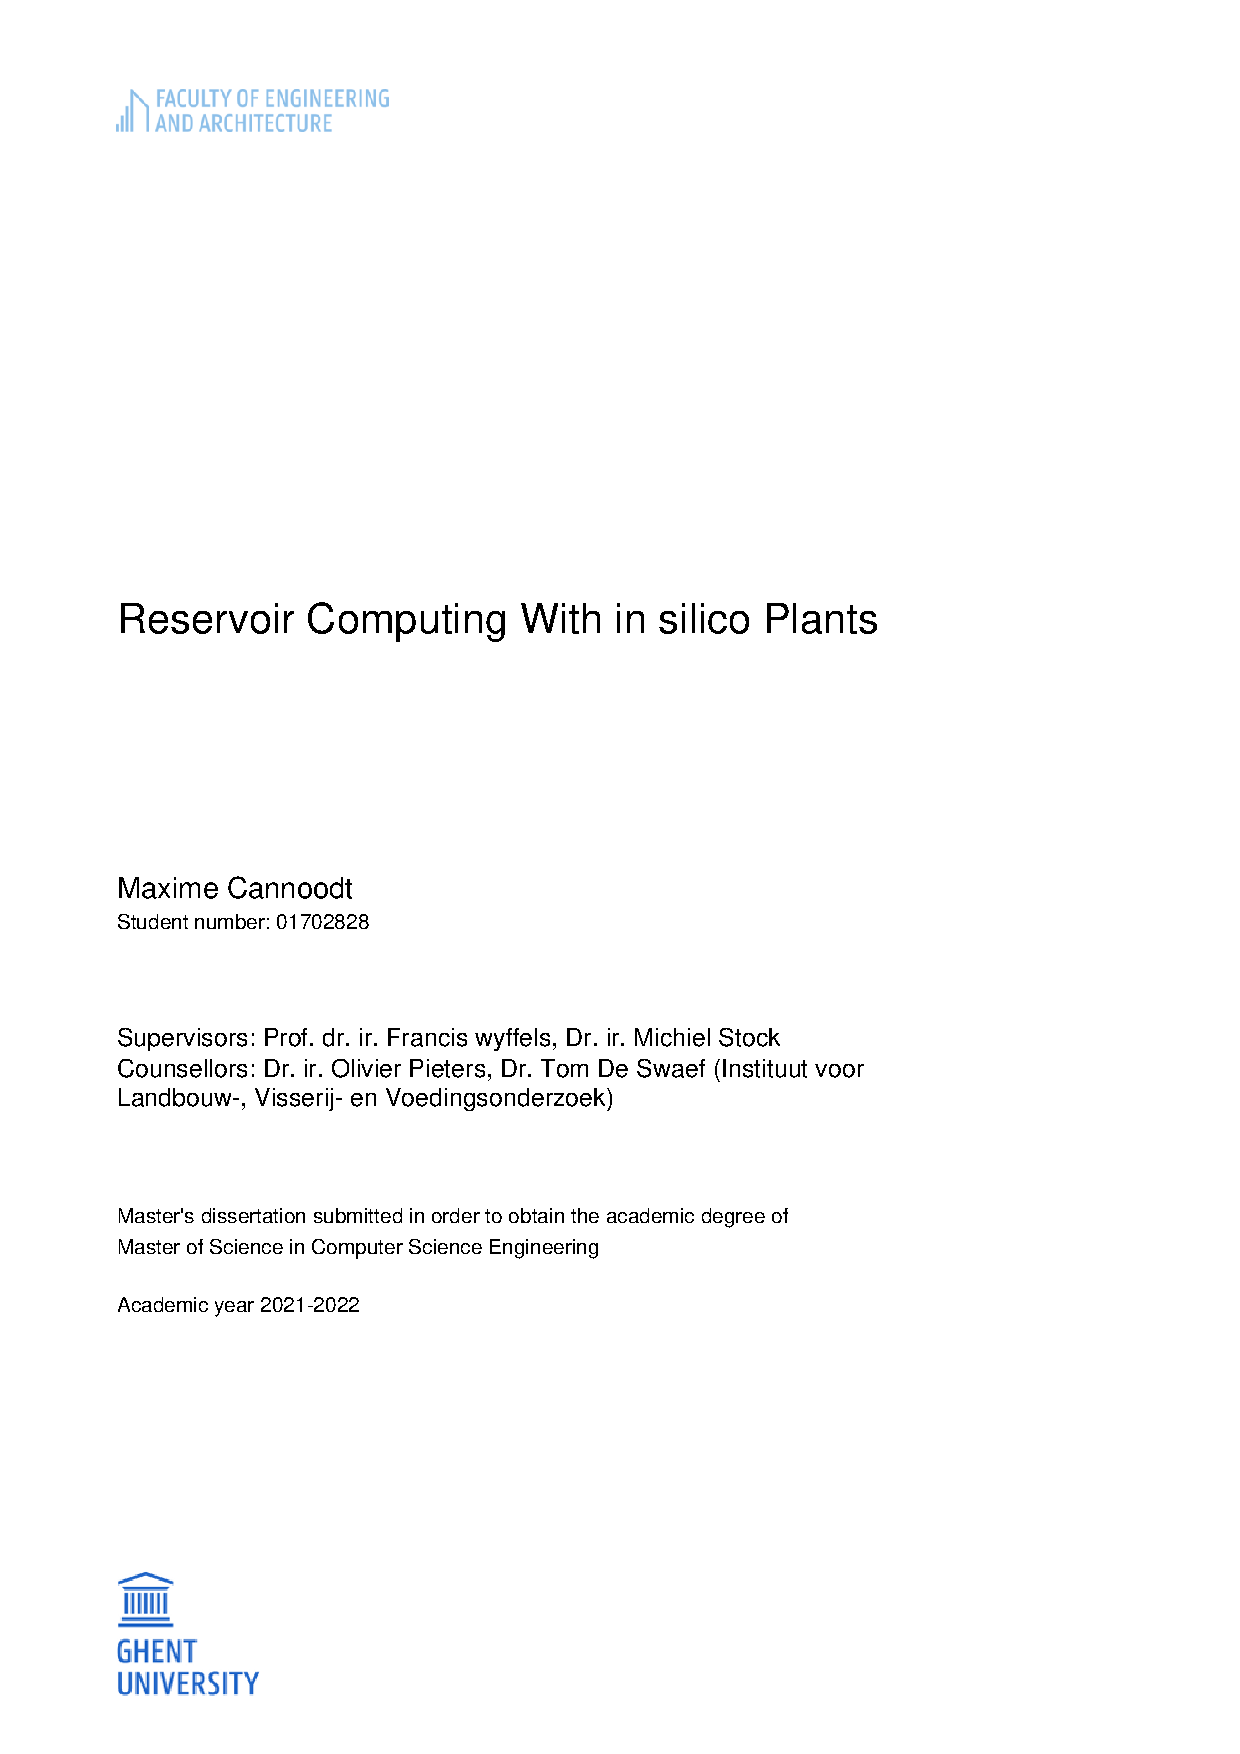
\includepdf[pages={1}]{cover-page-plato.pdf}

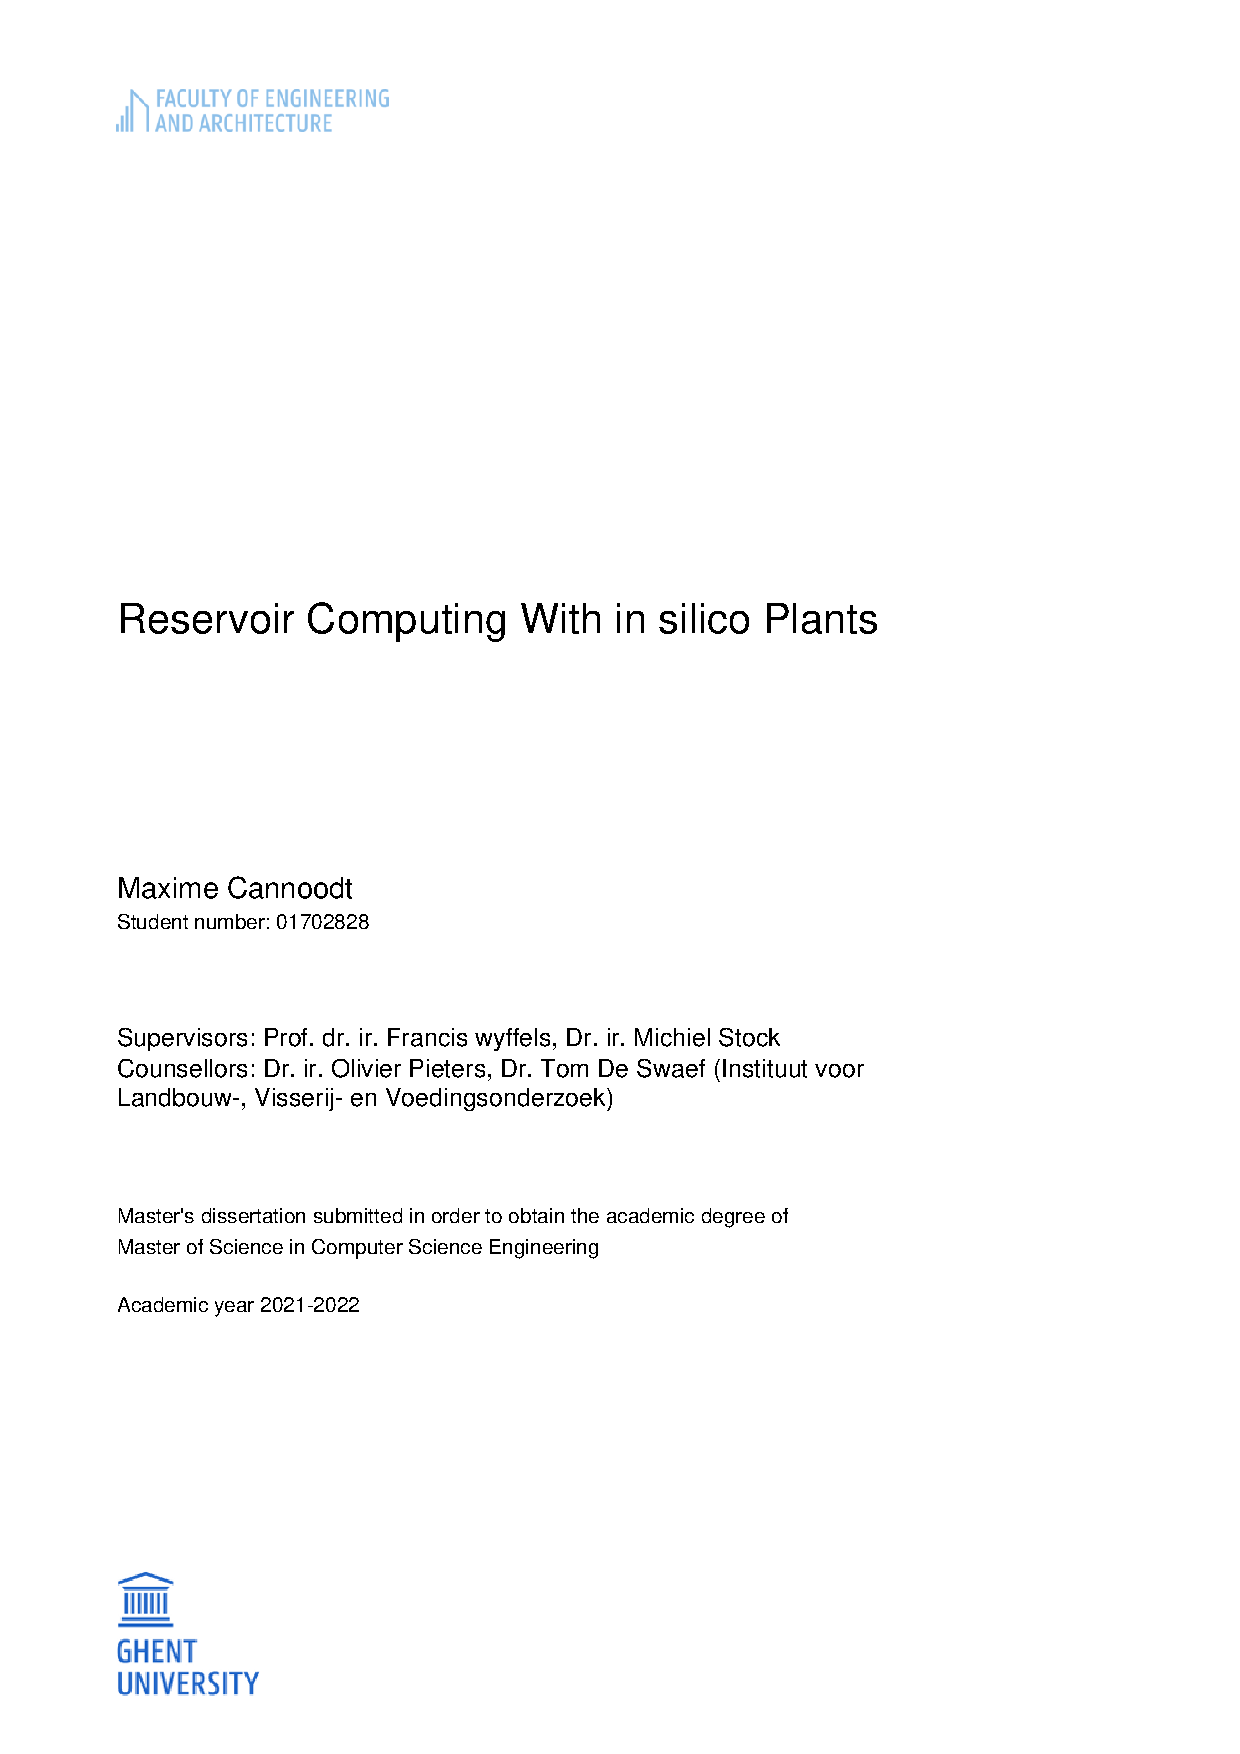
\includepdf[pages={1}]{cover-page-plato.pdf}

\restoregeometry
\newpage
    
\fontsize{10pt}{14pt}\selectfont

%%%%%%%%%%%%%%%%%
%% FRONTMATTER %%
%%%%%%%%%%%%%%%%%
\frontmatter

\newpage
\fancyhf{} % Clear header/footer
% \renewcommand{\headrulewidth}{0pt}
\pagenumbering{gobble}
This master's dissertation is part of an exam. Any comments formulated by the assessment
committee during the oral presentation of the master's dissertation are not included in this
text.
\vspace{0.5cm}

The author gives permission to make this master dissertation available for consultation and to copy parts of this master dissertation for personal use.
In all cases of other use, the copyright terms have to be respected, in particular with regard to the obligation to state explicitly the source when quoting results from this master dissertation.

\vspace{1cm}
\begin{flushright}
Maxime Cannoodt \\
May 26, 2022
\end{flushright}

\newpage

% To clear page numbers from footer, and header line at the start of every chapter
\fancypagestyle{plain}{\fancyhf{}\renewcommand{\headrulewidth}{0pt}} 
\pagestyle{fancy}
\fancyhf{} % Clear header/footer
\fancyhead[L]{\nouppercase\leftmark}
\cfoot{\thepage}
\pagenumbering{roman}


% Acknowledgments
\chapter*{Acknowledgments} \label{chapter:ack}
\addcontentsline{toc}{chapter}{Acknowledgments}

I would like to express gratitude towards the people without whom this thesis would not have been possible.

% - [ ] Olivier for a lot of feedback on my writing and providing an very good basis to work from
% - [ ] Francis for challenging my understanding of the research and bringing good new ideas to try when I was stuck.
First, I want to thank my counselor and advisor Olivier Pieters. 
The feedback he provided on the countless iterations of this book has been invaluable to the end product.
I wish to thank my promotor Francis wyffels for continuously challenging my understanding of my research results and coming up with new ideas to try when I felt like I reached a dead end.
I want to thank both of them especially for introducing me to the topic of reservoir computing.
It was certainly an unconventional pick from the list of dissertation topics, 
but every time I saw my peers struggle to stay interested in their subjects, I was glad I chose the unbeaten path.

% - [ ] Tom de swaef for explaining biological things and plant modelling concepts.
% - [ ] WUR/OnePlanet for the invitation to the meeting and tour of their phenotyping facility
% - [ ] Albasha for the feedback on the HydroShoot FSPM
I also want to thank Tom De Swaef for filling the gaps in my biological knowledge and helping me understand concepts in computer plant modeling.
Rami Albasha deserves a special mention for answering my questions about the inner workings of their grapevine simulation.
And thanks, Francis and OnePlanet Research Center, for inviting me to their research meeting.
Visiting WUR's phenotyping facilities and listening to their active projects helped me understand better how plant reservoir computing fits in the landscape of agricultural technology.

% - [ ] Jone & Tom for moral support, work group and sanity
% - [ ] Felix for moral support, sanity
Finally, I want to show gratitude to the people who have accompanied me during this arduous journey. 
Thank you to Jone Hoong and Tom for the social work sessions on Wednesdays and Thursdays at the iGent tower.
I admit I might have distracted you two more than I should have, but the weekly social interaction helped me stay sane as we slowly worked towards our finished thesis books.
My boyfriend Felix deserves a massive thank you for his patience when I worked late into the night and for listening to me vent my frustrations when progress was slow, or results were not as expected.
Last but not least, I want to thank my family for their patience when I was more distant and absent during this academic year.
I have always struggled to find the right balance between school and family, but now we can finally celebrate the end!


\vspace{0.5cm}

This dissertation topic challenged me to change my belief about what computation means.
After seven months of research, I hope that I can explain the concepts of plant reservoir computing to you in an accessible way. 
I believe that we are only at the beginning of the road for plant reservoir computing.
If the knowledge and technology can scale, I find the opportunities in agricultural tech immensely exciting.
 

% Abstract
\chapter*{Abstract} \label{chapter:abstract}
\addcontentsline{toc}{chapter}{Abstract}
We present a framework to evaluate the computational capabilities of plant physiological processes in plant models for physical reservoir computing (PRC).
PRC is a computing paradigm that enables the use of physical substrates for computation. 
% Recently, the use of live plants in a PRC context was demonstrated. 
Recently, Pieters (2022) proposed and successfully demonstrated the use of plants in a PRC context.
We expand upon this work \textit{in silico} using plant models for grapevine and wheat. 
The use of computer simulations gave us the freedom to observe the plant directly, without the need for sensing technology and laboratory setups.
In our experiments, we investigated the use of leaf temperature, transpiration rate, photosynthesis rate, light absorption, water flow, and hydraulic pressure as readout traits. 
Each of these traits displayed reservoir dynamics and correlated well with biologically relevant tasks. 
Surprisingly, our framework highlighted unusual behavior in mechanistic plant models, which the authors did not yet report.
We propose that the plant-modeling community can adapt the methods in this work to verify the behavior of plant models. 
We believe that this is just the starting point for plant reservoir computing.
If knowledge and technology can scale, there will be countless opportunities in agricultural technology.




% % **Goals:**
% Physical reservoir computing (PRC) is a machine learning method that exploits physical materials to perform computations.
% PRC has enjoyed success in domains such as soft body robotics and photonic circuits.
% In this thesis, we continue his work.
% We set out to identify which plant physiological processes display emergent computational qualities.
% To this end, we present a framework for making a quantitative comparison of plant physiological reservoirs.
% % **Methods:**
% We applied this framework with \textit{in silico} plants;
% we used existing mechanistic models of grapevine and common wheat found in the literature.
% Consequently, it sped up the research process and gave us a first intuition about suitable plant reservoirs.
% Our experiments evaluated the computational properties of leaf temperature, transpiration rate, photosynthesis rate, light absorption, water flow, and hydraulic pressure.
% % **Results:**
% Each of these physiological processes showed reservoir dynamics and correlated well with biologically relevant tasks.
% As a side effect, our framework uncovered flaws and unusual behavior in the mechanistic plant models that were previously unreported.
% We suggest that the plant-modeling community can adapt the methods in this thesis to verify the behavior of plant models.

\vspace{.5cm}
\textbf{Keywords:} Physical Reservoir Computing (PRC), Unconventional Computing, Plant Physiology, functional-structural plant models (FSPMs).

% - Physical reservoir computing is a machine learning method for performing computations with physical substrates.
% - PRC has seen succesful applications in e.g.\ compliant robots and photonic circuits.
% - Recently, Pieters (2022) proposed the use of plants as a reservoir medium.
% - In this work we set out to identify plant physiological processes that display emergent computational qualities.
% - More specifically we propose a framework to quantitatively compare the reservoir properties of plant physiological processes.

% - In this thesis we used mechanistic plant models as our test subjects
% - Specifically, we used a model of grapevine and a model of common wheat.
% - Four our experiments, we compare the properties of ..., ..., … and … .

% - Our experiments showed promising results for the future of plant reservoir computing.
% - However, the quality of our data was limited by the time resolution of the used plant simulations,
% - As a side effect, our framework was able to highlight flaws and unusual behavior in the used mechanistic models. 

% Extended abstract
\addcontentsline{toc}{chapter}{Extended Abstract}
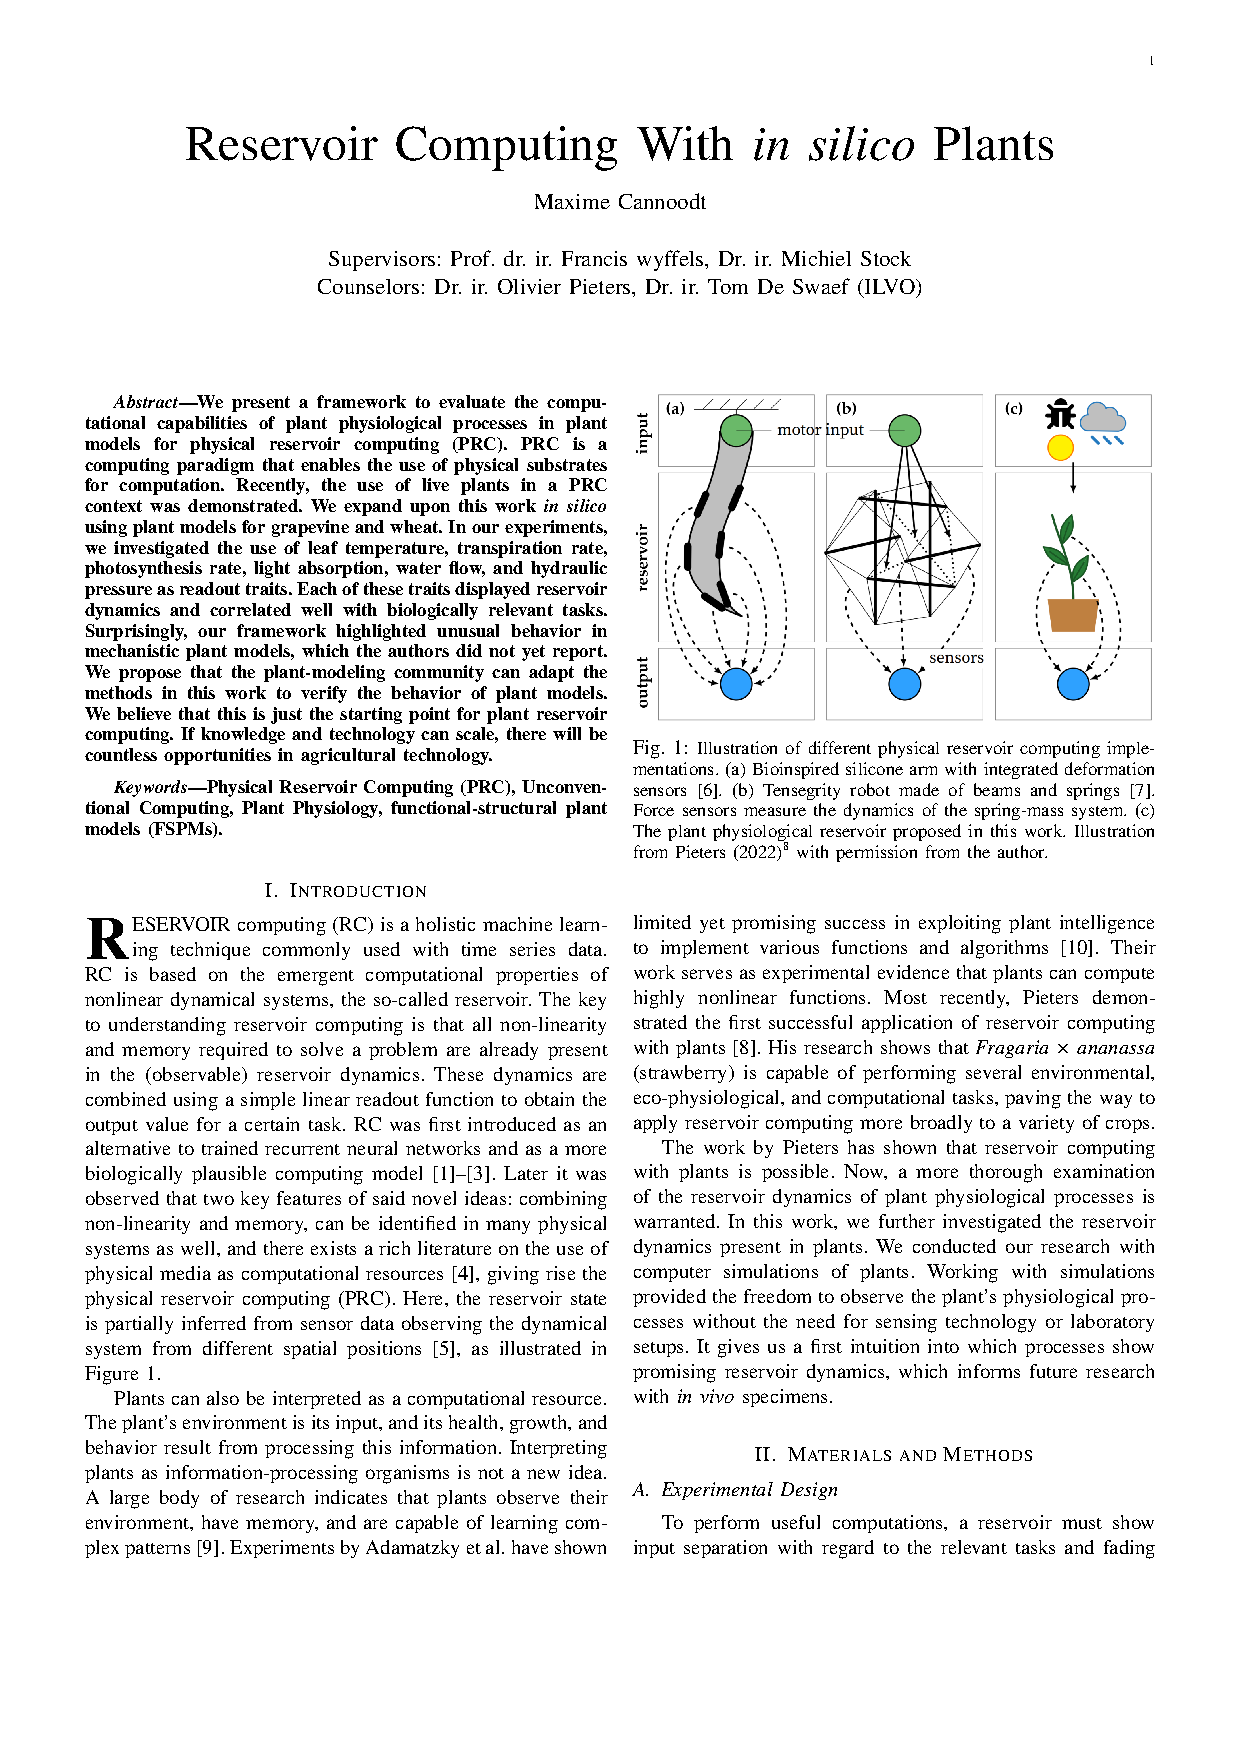
\includepdf[pages=-]{thesis_extended_abstract.pdf}

% Table of contents
\clearpage
% \singlespacing
\setcounter{tocdepth}{2}
\addcontentsline{toc}{chapter}{Contents}
\tableofcontents
\newpage

% Tables and figures
\addcontentsline{toc}{chapter}{List of Figures}
\listoffigures
\addcontentsline{toc}{chapter}{List of Tables}
\listoftables

% Abbreviations and symbols
\addcontentsline{toc}{chapter}{Acronyms}
\newacronym{rc}{RC}{Reservoir Computing}

\newacronym{rnn}{RNN}{Recurrent Neural Network}

\newacronym{bptt}{BPTT}{Backpropagation-Through-Time}

\newacronym{esn}{ESN}{Echo State Network}

\newacronym{lsm}{LSM}{Liquid State Network}

\newacronym{bpdc}{BPDC}{Backpropagation-Decorrelation}

\newacronym{prc}{PRC}{Physical Reservoir Computing}

\newacronym{fpga}{FPGA}{Field-Programmable Gate Array}

\newacronym{esp}{ESP}{Echo State Property}

\newacronym{csm}{CSM}{Crop Surface Model}

\newacronym{fspm}{FSPM}{Functional-Structural Plant Model}

\newacronym{narma}{NARMA}{Nonlinear Autoregressive Moving Average}

\newacronym{mse}{MSE}{Mean Squared Error}

\newacronym{nmse}{NMSE}{Normalized Mean Square Error}

\newacronym{par}{PAR}{Photosynthetically active radiation}

\printglossary[type=\acronymtype]


%%%%%%%%%%%%%%%%
%% MAINMATTER %%
%%%%%%%%%%%%%%%%
\mainmatter

\part{Background}

\chapter{Introduction} \label{chapter:intro}

% Intro to a background in agricultural research
New challenges confront the field of agricultural research every year.
The biggest challenge is, of course, climate change \citep{bisoffi_meta-analysis_2019}.
% While changing climate conditions threaten agricultural activities, farming practices themselves play a significant role in climate change \cite{bisoffi_meta-analysis_2019}.
Changing climate conditions threaten many common crops, including staple crops such as corn, wheat, rice, sunflower, and cotton \citep{hatfield_ch_2014}.
Other areas of concern include food security, rising population, declining land productivity, and urban food strategy \citep{european_commission_directorate_general_for_research_and_innovation_new_2009, european_commission_directorate_general_for_research_and_innovation_resilience_2020}.

\section{Ongoing Efforts in Agricultural Research}

% Intro to phenotyping: definition, role in research, link with agriculture challenges
A significant amount of research is dedicated to discovering and breeding crop varieties that are well-adapted to the novel climate, water, and soil conditions caused by global warming.
Phenotyping plays a vital role in this.
In agricultural research, phenotyping refers to identifying species varieties (phenotypes) with positive traits from a large pool of genetic variants (genotypes) \citep{walter_plant_2015}.
For example, suppose researchers attempt to breed crops more resilient to saltwater. 
In that case, the researchers will measure the saltwater resistance of each specimen in their pool of genetic variants and selectively breed the phenotypes with the best resistive properties.
However, the phenotype of an organism is the outcome of complex interactions between genetic and environmental factors, resulting in a high-dimensional problem space \citep{walter_plant_2015}. 
Because of this, current \textit{in vivo} research is limited to measuring the effect of one or two environmental variables on a plant, even though the plant's response integrates many more variables that are unaccounted for \citep{pieters_reservoir_2022}. 
Novel approaches should aim to more accurately model the interaction between the phenotype and the whole environment.


% Intro to autonomous farming
Another active line of research is autonomous greenhouse farming.
Crop growth in a greenhouse setting is affected by many factors, including light, temperature, humidity, CO\textsubscript{2}, and water and nutrient delivery \citep{hemming_why_nodate}.
The greenhouse farmer must finely control these factors to balance crop yield with major cost drivers like water and energy intensity.
In addition, the grower must control pests and diseases to have a successful harvest.
A farmer who wishes to optimize their operating efficiency must manage all these interlinked aspects, which requires an intricate understanding of the crop species from the grower.
The need for this deep, crop-specific domain knowledge forms a bottleneck for rapidly expanding the number of greenhouses in operation or scaling the number of different crops grown in a single facility.
Autonomous farming aims to assist the farmer through (partial) automation of the decision-making process and delivery system while minimizing resource use.
This goal can be achieved using advanced sensor technology combined with AI techniques such as computer vision and machine learning \citep{hemming_why_nodate}.
Autonomous greenhouses may one day answer the need for food security and food delivery in areas with high urban density and decrease the strain on rural farmlands to feed the rapidly growing urban population.


% Intro to the need for a better understanding of plant physiology
On a more fundamental level, research must be conducted to better understand the eco-physiological processes that drive plant growth and health.
A better understanding of the inner workings of plants will help accelerate the development of new resistant varieties.
It can also help reveal the soundest indicators of plant well-being to incorporate into the control systems of autonomous greenhouses.
Yet, it is insufficient to comprehend the physical interactions between the plant and its abiotic environment in isolation.
The plant responds to the sum of its environment, resulting in emergent behavior that may be unaccounted for in theoretical findings and lab experiments \citep{poorter_pampered_2016}.


% The state of modeling plant-environment interactions
Mechanistic models are state-of-the-art for modeling the interactions between the plant and its abiotic environment. 
These models simulate the plant at the lowest level, commonly implementing physiological processes at the cell organ level such as photosynthesis, transpiration, and water and carbon flow \citep{coussement_turgor-driven_2020}.
It then becomes possible to study emergent behaviors that result from these base processes.
By subjecting mechanistic models to novel environmental conditions, they can simulate the plant's response to various scenarios, such as new soil types or drought.
This use case makes mechanistic models of particular interest in understanding macroscopic plant behavior and phenotyping.
This type of model has shown very encouraging results in the past decade \citep{louarn_two_2020}.


However, there are some drawbacks to mechanistic models.
First, this model is computationally expensive as it relies on solving many differential equations for every time step. 
Because of this, the simulated time scale is frequently limited to hours or days. The computational cost makes them unsuited for modeling interactions that occur at the second or minute scale, even though those play a significant role in the behavior of plants \citep{pieters_reservoir_2022}.
Second, the development of mechanistic models is closely coupled to the theoretical understanding of a species's physiology. 
As a result, the model is only as accurate as the current understanding of the plant's low-level processes.
Finally, developing a mechanistic model is a significant undertaking. 
A large portion of the work cannot be generalized to other species, which forms a significant bottleneck in the development speed of plant models.
In conclusion, though mechanistic models have become increasingly relevant in the literature, there is still room for alternative approaches that can be applied more broadly and are faster to deploy.

\section{Reservoir Computing}

% What is reservoir computing?
\acrfull{rc} is a holistic machine learning technique commonly used with time series data.
Instead of relying on resource-intensive and data-hungry deep learning techniques, \acrshort{rc} works by exploiting the computational properties of nonlinear dynamical systems, which are called reservoirs in this context.
The key to understanding reservoir computing is that all non-linearity and memory required to solve a problem are already present in the reservoir dynamics.
Only a simple linear regression model is needed to transform the information in the reservoir into an interpretable output value.
\acrshort{rc} was first introduced as a computer model \citep{jaeger_echo_2002, maass_real-time_2002, steil_backpropagation-decorrelation_2004}.
However, nonlinear dynamical behavior can be observed in many physical systems as well, and there exists a rich literature on the use of physical media as computational resources \citep{tanaka_recent_2019}.


% What is reservoir computing with plants?
Plants can also be interpreted as a computational resource.
The plant's environment is the its input, and its health, growth, and behavior are a result of processing this information.
Interpreting plants as intelligent information-processing organisms is not a new idea.
A large body of research indicates that plants are aware of their environment, have memory, and are capable of learning complex patterns \citep{mancuso_revolutionary_2018}. 
Experiments by \citet{stepney_computers_2018} have shown limited yet promising success in exploiting plant intelligence to implement various functions and algorithms.
Though our goal is not to implement general-purpose computing using plants, their work serves as experimental evidence that plants can indeed compute highly nonlinear functions.
Most recently, \citet{pieters_plants_2021} have demonstrated the first successful application of reservoir computing with plants. 
Their research shows that \textit{Fragaria × ananassa} (strawberry) is capable of performing several environmental, eco-physiological, and computational tasks, paving the way to apply reservoir computing more broadly to a variety of crops.


% Applications of reservoir computing with plants?
If plants do indeed behave like computing reservoirs, \acrshort{rc} may become a versatile addition to the agricultural research and development toolbox.
For example, observing and measuring the relationship between environmental signals (reservoir input) and plant behavior (reservoir dynamics), we could gain insights into eco-physiological processes not yet uncovered or understood.
We suspect there are still considerable opportunities for discovering new phenomena with this holistic data-driven approach, especially on the time scale between seconds and minutes.
In addition, reservoir computing can have applications in phenotyping. 
The \acrshort{rc} framework may be able to identify phenotypes that are better or faster at integrating their environmental inputs into an adaptive response.
Especially rapid responses are currently underexplored in phenotyping research, even though they play an essential role in plant life \citep{alarcon_substantial_1994, de_swaef_plant_2015}.
Even further down the road, RC can be applied in autonomous greenhouses to observe the plant's real-time response to the conditions set by the grower or autonomous control system. 
A closed-circuit control loop can be designed that integrates the real-time behavior of the plant, where the plant itself controls the delivery of light, water, and nutrients.


\section{Research Outline}

% Outline of my research contribution
% \citet{pieters_reservoir_2022} has shown that reservoir computing with plants is possible.
% Now, a more thorough examination of the reservoir characteristics of plant-physiological processes is warranted.
% The main contribution of this work is the further exploration of the available reservoir dynamics in plants.
% We investigate several observable eco-physiological processes' nonlinearity, memory capacity, and fading memory property by performing relevant environmental and eco-physiological reservoir tasks. 
% We identify a set of promising physiological processes as reservoirs for future \acrshort{rc} research.
The work by Pieters has shown that reservoir computing with plants is possible.
Now, a more thorough examination of the reservoir characteristics of plant-physiological processes is warranted.
In this work, we further investigated the reservoir dynamics present in plants.
We investigated several observable eco-physiological processes' linear task separation and memory capacity by performing relevant environmental and eco-physiological reservoir tasks. 
These experiments identified a set of promising physiological reservoirs for future RC research.
We also verified whether these physiological processes displayed the fading memory property, an essential precondition for performing deterministic computations.


% Why in silico plants?
We conduct our research with \textit{in silico} plants.
Working with simulations provides the freedom to observe the plant's physiological processes without the need for sensing technology or laboratory setups.
% It gives us a first intuition into which processes show promising reservoir dynamics, which directly informs future plant \acrshort{rc} research with \textit{in vivo} specimens.
% \acrshort{rc} might also contribute to FSPM development by identifying weaknesses in models that have previously gone unnoticed.
It gives us a first intuition into which processes show promising reservoir dynamics, which informs future research with \textit{in vivo} specimens.
RC can also contribute to FSPM development by identifying flaws in physiological models that previously went unnoticed.


\newpage
\section{Chapters overview}

To understand the research presented in this book, Chapter \ref{chapter:lit-prc} starts with a brief primer on the principles of reservoir computing and the use of physical media for computation. 
In Chapter \ref{chapter:fspm}, we give a brief introduction to the research field of plant modeling and simulation. 
Then, Chapter \ref{chapter:exp-setup} elaborates on the research goals set for this work and explains the experimental design.
Chapters \ref{chapter:models-used} and \ref{chapter:methods} delve deeper into our methods by explaining the selection process for computer plant models and the experiment implementation details, respectively.
Next, Chapter \ref{chapter:results} reports our experimental data and discusses those results. 
Finally, \ref{chapter:discussion} concludes the book with a summary of our key takeaways and a discussion of future work.

\chapter{Physical Reservoir Computing} \label{chapter:lit-prc}

\section{Reservoir Computing} \label{section:rc}
% Where does RC come from?
Reservoir computing (\acrshort{rc}) is a machine learning method proposed in the early 2000s as an alternative to training recurrent neural networks (\acrshort{rnn}) \citep{jaeger_echo_2002}. 
Training weights in recurrent networks requires computationally expensive and highly linear training algorithms such as backpropagation-through-time (\acrshort{bptt}). 
Moreover, \acrshort{bptt} often suffers from numerical instability and often yields suboptimal solutions \citep{bengio_learning_1994}.

In the \acrshort{rc} framework, the untrained \acrshort{rnn} (called the reservoir) is interpreted as a black box dynamical system.
Input signals are transformed by the nonlinear activations of the neurons and are integrated with the past state of the reservoir through recurrent connections \citep{jaeger_harnessing_2004}.
As a result, the reservoir displays both nonlinear behavior and memory capacity.
We can then exploit these properties to solve a variety of regression tasks.


% What does an RC model look like?
\mbox{Figure \ref{fig:rc_diagram}} shows a diagram of a general \acrshort{rc} model using an \acrshort{rnn} as the reservoir.
To accomplish regression tasks, an \acrshort{rc} model consists of two parts: the nonlinear reservoir that transforms environmental inputs and a linear readout function that observes the reservoir to perform a given task. 
The linear readout function observes the state of the reservoir and applies a linear regression model to determine the final output. 
When there is no feedback from the readout function back to the reservoir, it is possible to train multiple readouts that perform different tasks based on the same reservoir dynamics.

\begin{figure}[t]
	\centering
    \includesvg[width=0.65\textwidth]{img/rnn-illustration.svg}
    \vspace{0.35cm}
    % \includegraphics[width=0.5\textwidth]{example-image}
	\caption[A reservoir computing model with a RNN as the reservoir, commonly referred to as an echo state network (ESN).]
	        {A reservoir computing model with a RNN as the reservoir, commonly referred to as an echo state network (ESN).
    	 	 Figure reproduced from \citet{pieters_reservoir_2022} with permission from the author.}
	\label{fig:rc_diagram}
\end{figure}


% What makes RC work?
The key to understanding reservoir computing is that all non-linearity and memory required to solve a given task are already present in the reservoir dynamics. 
The readout function then learns to distill the information present in the observed reservoir state to solve a given task. 
In this way, \acrshort{rc} is similar to the kernel method from classical machine learning, where the reservoir acts as a nonlinear expansion and temporal convolution of the input signals \citep{hermans_recurrent_2012}. 
However, kernel techniques do not account for time explicitly, whereas reservoir computing inherently occurs in the time domain. 
This strong connection to the time domain makes \acrshort{rc} particularly useful for solving tasks with time series data and real-time applications.


% RC is data-efficient and easier to train.
In its original form, the neurons inside the reservoir are randomly connected and are generally not trained. 
However, there is literature that proposes task-independent tuning schemes that improve the stability of the reservoir \citep{lukosevicius_reservoir_2009, norton_preparing_2006, tanaka_effect_2020}.
Reservoir computing models are notably more data-efficient and easier to train because there is no need to train the recurrent part of the network using complex and data-hungry algorithms such as \acrshort{bptt}.


% Concrete frameworks for implementing reservoir computing.
The literature has proposed several implementations of reservoirs.
The echo state network (\acrshort{esn}), as proposed by \citet{jaeger_echo_2002}, is a purely mathematical implementation where neuron activations are determined as a nonlinear function of the weighted sum of incoming connections. 
\acrshort{esn}s operate in discrete time only and are ideal for software implementations.
Subsection \ref{subsection:esn} gives a detailed mathematical description of the echo state network.
Independently, \citet{maass_real-time_2002} proposed the liquid state machine (\acrshort{lsm}), an idea that originated from computational neuroscience.
In this model, the recurrent network is formed by spiking neurons that can operate in both discrete and continuous time.
The neurons receive spike trains (discrete events in time) as input and generate an output sequence of spikes accordingly.
A third approach proposed by \citet{steil_backpropagation-decorrelation_2004} is called Backpropagation-Decorrelation (\acrshort{bpdc}). 
It is a learning algorithm for online training of the readout weights.


\subsection{Echo State Network} \label{subsection:esn}


% introduction
The Echo State Network (ESN) is a mathematical framework that implements the core concepts of reservoir computing \citep{jaeger_tutorial_2002}. 
In this framework, the reservoir is a discrete-time RNN using a sigmoidal nonlinearity (such as the tanh function). 
The activation weights of the reservoir are initialized randomly and remain fixed. 
The linear readout function takes the reservoir state as input and is fit to the desired target signal.

The reservoir state in time step $t$ is calculated from the input signal $\mathbf{u}$ using the following update rules \citep{lukosevicius_reservoir_2012},


\begin{align}
    \tilde{\mathbf{x}}[t] &= \tanh \left( \mathbf{W}^{\text{in}}[1;\mathbf{u}[t]] + \mathbf{W} \mathbf{x}[t-1] \right) \label{esn:update1} \\
    \mathbf{x}[t] &= (1-\alpha) \mathbf{x}[t-1] + \alpha \tilde{\mathbf{x}}[t] \label{esn:update2}
\end{align}


where $\mathbf{x}$ signifies the reservoir neurons' activations, $\mathbf{\tilde{x}}$ the activation update, and $\alpha$ a scalar leaking rate. The readout function $\mathbf{y}$ is fulfilled by a simple linear regression of the reservoir state and an optional direct feed-in of the input signal.

\begin{equation}
\mathbf{y}[t] = \mathbf{W}^{\text{out}}\left[1; \mathbf{u}[t];\mathbf{x}[t] \right] \label{esn:readout}
\end{equation}


The weights $\mathbf{W}^{\text{out}}$ of the readout function can be trained using a variety of learning methods. A common offline approach for fitting the function output to a target signal is ridge regression \citep{lukosevicius_reservoir_2012}:

\begin{equation}
    \mathbf{W}^{\text{out}} = \mathbf{Y}_{\text{target}}\mathbf{X}^{T} \left(\mathbf{X} \mathbf{X}^{T} + \lambda^{2} \mathbf{I} \right)^{-1} \label{esn:training}
\end{equation}

where $\lambda$ is a regularization parameter that prevents overfitting.
For $\lambda$ = 0, the model attempts to find weights that fit the training data exactly.
The results is a high training accuracy, but low accuracy on unseen data.
Large model weights are penalized for $\lambda$ > 0, resulting in smaller weights and a more generalized model.
However, if $\lambda$ is too large, the model parameters shrink too much, and the model loses expressiveness.
The optimal value for $\lambda$ should be selected using validation data separate from training and test data.
Other regression techniques are also possible.
For example, \citet{burms_reward-modulated_2015} have demonstrated online training of the readout function using reward-modulated Hebbian plasticity rules.


\subsection{Applications} \label{subsection:rc_applications}


% Introduction to application domains.
Reservoir computing has enjoyed success in a multitude of research domains because of its simple computational model, the potential for real-time processing, and broad applicability to problems in the physical world \citep{tanaka_recent_2019}. 
Early applications of RC include time series prediction tasks such as stock price forecasting and weather forecasting \citep{nakajima_physical_2020}. 
Table \ref{table:rc-subjects} shows a comprehensive summary of the domains to which RC has been applied as compiled by \citet{tanaka_recent_2019}.
Similarly, \mbox{Table \ref{table:rc-applications-benchmarks}} gives a selection of works that demonstrate the application of reservoir computing. 


\input{tables/tanaka-table1-rc-subjects}

\input{tables/tanaka-table2-rc-applications-benchmarks}

% Tables \ref{table:rc-subjects} and \ref{table:rc-applications-benchmarks} give an overview of subjects to which RC has been applied and references to applications and benchmarks respectively.
% In robotics, RC is deployed as a low-power real-time integrator of sensor data and motor controller  \citep{nakajima_information_2015, burms_reward-modulated_2015}.



% \ref{table:rc-subjects}

% One of the earliest demonstrations of reservoir computing is the Liquid State Machine (2002)\citep{maass_real-time_2002}.

% Since its inception, reservoir computing has been successfully applied in several domains. % though today it has mostly been succeeded by Deep Learning techniques \cite{citation needed}.

% - Example of LSM \cite{maass_real-time_2002}

% - Examples of applications are \cite{lukosevicius_reservoir_2012, nakajima_physical_2020}. see also Tanaka 2019 section 2.2 table 1 and table 2 \cite{tanaka_recent_2019}.

% - Also the source of more theoretical research in mathematics and chaos, see \cite{hermans_recurrent_2012, gauthier_next_2021}

  

\section{Physical Reservoir Computing} \label{section:prc}

% What is physical reservoir computing?
The RC model easily extends to the physical world by interpreting physical systems that exhibit nonlinear dynamics and memory effects as a reservoir substrate  \citep{nakajima_physical_2020}. 
In other words, this Physical Reservoir Computing (PRC) framework aims to exploit dynamics found in the natural world to perform computational tasks. 
% How is RC transferred to the real world?
\mbox{Figure \ref{fig:prc_examples}} shows a mapping of the RNN-based RC architecture to two physical applications from the literature and the plant RC case discussed in this thesis.
In the physical systems (\mbox{Figures \ref{fig:prc_examples}}b, c, and d), it is impossible to observe the complete state of the reservoir as in the RNN-based reservoir. 
Instead, the reservoir state is inferred from sensor data observing the dynamical system in real-time \citep{burms_reward-modulated_2015, nakajima_information_2015}.

\begin{figure}[t]
	\centering
    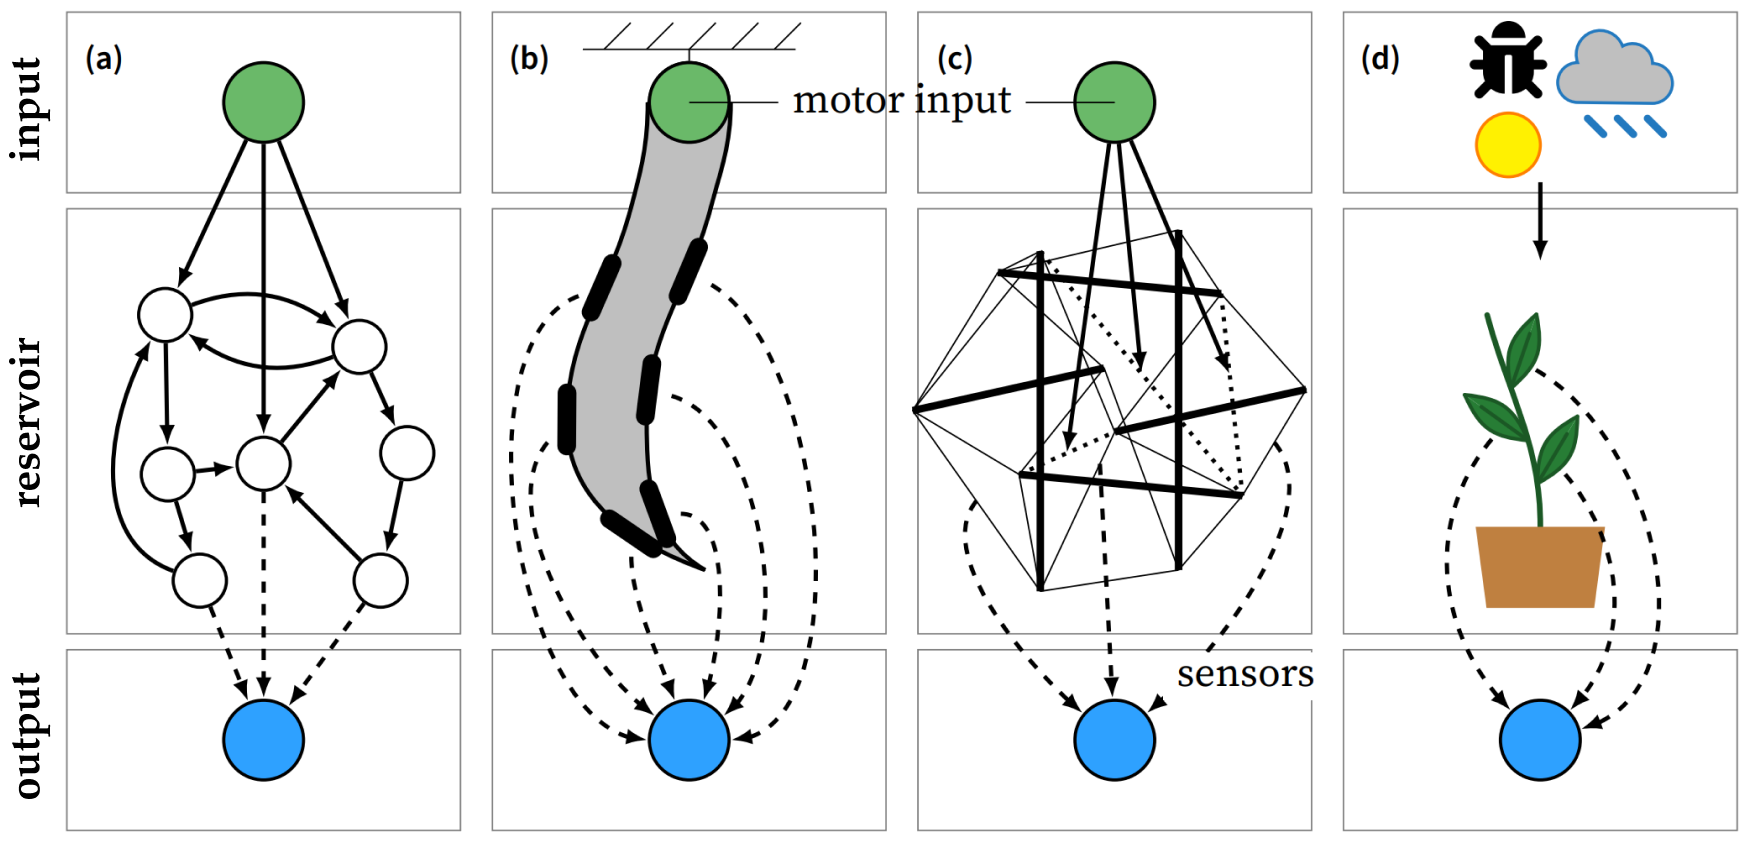
\includegraphics[width=0.9\textwidth]{img/prc-illustration.png}
    % \vspace{0.5cm}
    % \includegraphics[width=0.5\textwidth]{example-image}
	\caption[Illustration of different reservoir computing implementations, both theoretical and physical versions.]
	        {Illustration of different reservoir computing implementations, both theoretical and physical versions. 
	        Each of the subfigures depicts a different type of implementation: 
	            (a) RNN-based version; 
	            (b) soft body built of silicone \citep{nakajima_information_2015}; 
	            (c) compliant robot made of a tensegrity structure \citep{caluwaerts_locomotion_2013}; 
	            and (d) plant as reservoir.
    	 	Figure and caption reused from \citet{pieters_reservoir_2022} with permission from the author.}
	\label{fig:prc_examples}
\end{figure}

% What applications have been made with PRC?
PRC is a field of interdisciplinary research, implementing reservoirs using a large variety of materials \citep{tanaka_recent_2019}.
Examples of substrates being researched are analog electrical circuits \citep{soriano_minimal_2015, zhao_novel_2016}, FPGAs \citep{antonik_application_2018}, memristive circuits \citep{walter_neuromorphic_2015}, photonic circuits \citep{van_der_sande_advances_2017}, spintronics \citep{torrejon_neuromorphic_2017}, and soft body robotics \citep{caluwaerts_body_2011, caluwaerts_design_2014, nakajima_soft_2013}.
Biological reservoirs are closely investigated as well, with a particular interest in neurobiology \citep{hafizovic_cmos-based_2007, hinaut_real-time_2013} and ecological dynamics \citep{jones_is_2007, didovyk_distributed_2015,ushio_computational_2021}. 
Most recently, \citet{pieters_plants_2021} demonstrated promising results in the use of \textit{in vivo} plants as reservoir substrate.


% What is the goal of PRC research?
A common misconception about PRC research is that the goal is to achieve general-purpose computation with unconventional reservoirs. 
However, the aim is not to outperform silicon computers at carrying out generic calculations. 
Instead, in most cases, the goal is to bypass the need for precise modeling of a physical system by observing how the system responds to inputs rather than attempting to predict how the inputs influence the state of the system \citep{nakajima_physical_2020}.
This method is particularly applicable in real-time control scenarios such as robotics, where real-time integration of sensor data is more feasible than power-hungry physics simulations (see e.g.\ \cite{caluwaerts_design_2014, burms_reward-modulated_2015}), 
or for the prediction of chaotic systems where powerful computers are not able to predict the system better than low-powered reservoir models \citep{gauthier_next_2021}.


\subsection{Generalized Mathematical Model} \label{section:rc-general}

The mathematical model of the Echo State Network (section \ref{subsection:esn}) can be generalized to describe any reservoir computer, physical or otherwise \citep{nakajima_physical_2020}. 
Doing so will be helpful to determine what defines the RC system's computational capacity in the following sections. 
This section establishes a mathematical vocabulary for describing any PRC model in discrete-time notation.

The reservoir update function can be described as a function $f(\cdot, \cdot)$ that maps the previous reservoir state and the current input to a new reservoir state,
 
\begin{equation} \label{prc:update}
    \mathbf{x}[t] = f\left(\mathbf{x}[t-1], \mathbf{u}[t]\right) 
\end{equation}

where $\mathbf{x}$ describes the entire reservoir state at step $t$ and $\mathbf{u}$ represents all external factors that influence the dynamics of the reservoir substrate. 
Assuming the reservoir dynamics result in emergent memory effects, it is possible to reformulate the reservoir state $\mathbf{x}$ as a function of the past inputs it has seen:

\begin{equation} \label{prc:echo_input_function}
    \mathbf{x}[t] = \phi(\mathbf{u}[t], \mathbf{u}[t-1], \mathbf{u}[t-2], \dots)
\end{equation}

This function $\phi$ is called the input echo function and is a key characteristic of each particular reservoir substrate. The target task is defined as any arbitrary function $T$ of the past time steps, thus requiring memory to solve:

\begin{equation} \label{prc:target}
    \mathbf{y}[t] = T(\mathbf{u}[t], \mathbf{u}[t-1], \mathbf{u}[t-2], \dots)
\end{equation}

Finally, the linear readout function $\psi$ is described as a learned approximation of $T$, based on the reservoir state:

\begin{align} 
    \psi(\mathbf{x}[t]) &= \psi \left( \phi(\mathbf{u}[t], \mathbf{u}[t-1], \mathbf{u}[t-2], \dots) \right) \label{prc:readout} \\
    &\approx T(\mathbf{u}[t], \mathbf{u}[t-1], \mathbf{u}[t-2], \dots) = \mathbf{y}[t] \nonumber
\end{align}

It is important to note that the input echo function $\phi$ is surjective for virtually all reservoirs. 
In other words, a unique sequence of inputs does not necessarily result in a sequence of unique reservoir states. 
Not only is this natural, as no reservoir can have infinite memory of past events, Section \ref{section:esp} shows that this summarizing property of $\phi$ is vital to derive any meaningful computation from reservoir computers. 

\section{The Echo State Property} \label{section:esp}

% Need for deterministic computations
Strictly speaking, for a reservoir to possess reproducible computational properties, it must show a deterministic relation between its input sequence and its state \citep{nakajima_physical_2020}. 
Put plainly, applying the same input sequence should reliably produce the same sequence of output states.


% Determinism is too strict for physical systems
This precondition is particularly strict on physical systems because it requires precise control over the initial conditions of the physical reservoir (Equation \ref{prc:update}).
This requirement is virtually unattainable as it is impossible to account for all physical factors of an environment that influence the reservoir before the start of the experiment.
Fortunately, a lesser but sufficient condition exists to perform useful computation with a reservoir.


% The echo state property comes to the rescue
The echo state property (\acrshort{esp}) (also referred to as the fading memory property) defines a less strict precondition under which it is possible to derive computations from a dynamical system.
Informally, the \acrshort{esp} states that a sufficient condition for reservoir computing is for the input echo function $\phi$ (Equation \ref{prc:echo_input_function}) to have fading memory of past inputs \citep{lukosevicius_reservoir_2012}. 
If this assumption is valid, then the trajectories of the reservoir state will converge when subjected to the same input sequence, regardless of the initial conditions.
A side-effect of the echo state property is that it limits the reservoir's memory of past events, thus limiting the available integration window for memory-bound tasks.


% Example in ESN.
Figure \ref{fig:fading_mem_principle} demonstrates the principle using an ESN. It shows the evolution of a single node in the network for two runs. 
At step 0, we initialized the reservoir state with a different random state vector. 
After step 0, we subject the reservoir to the same input sequence for both scenarios.
While the initial trajectory depends on the node's starting value, the neuron synchronizes to the input sequence entirely by step 75. 
The node's evolution no longer depends on the initial value from that point onwards.



% Fading memory can be recognized in many systems
Fading memory can be recognized in physical dynamical systems as well.
Oftentimes it is the result of a dampening force such as electrical resistance or drag.
For example, \citet{nakajima_information_2015} implemented \acrshort{prc} using a silicone octopus arm submerged in water. 
In their particular case, the. fluid resistance of the water tank exerts a dampening effect on the silicone arm, resulting in a fading memory.


% The mathematical reason why this works is still being researched
The understanding behind this property is that the response of many dynamical systems eventually synchronizes to the input signal, suppressing chaotic behavior \citep{nakajima_physical_2020}. 
However, the mathematical understanding of the \acrshort{esp} and its relation to dynamical systems is still a topic of active research (see e.g.\ \cite{yildiz_re-visiting_2012, lu_attractor_2018}).

\begin{figure}
    \centering
    \begin{subfigure}[b]{0.35\linewidth}
        \centering
        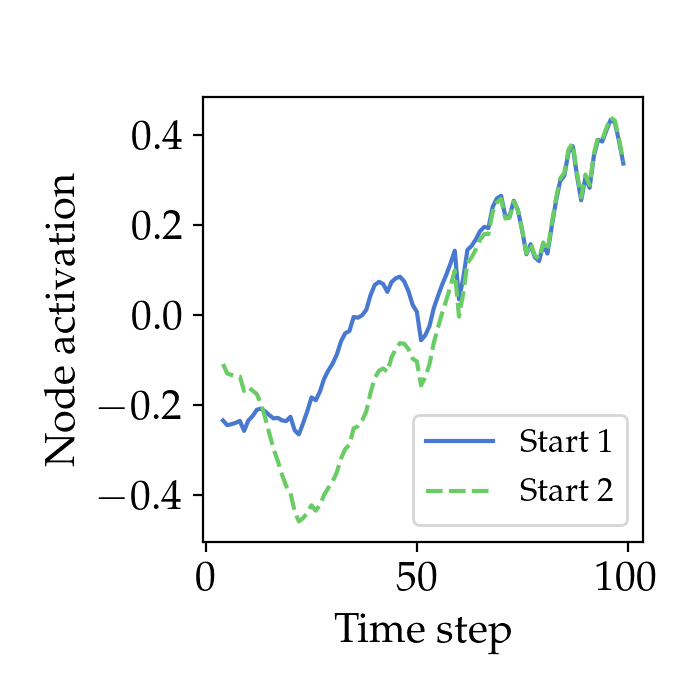
\includegraphics[height=5.7cm,keepaspectratio]{img/explainer_fading_mem.png}
        \caption{ }
        \label{fig:fading_mem_principle}
    \end{subfigure}
    \hfill
    \begin{subfigure}[b]{0.62\linewidth}
        \centering
        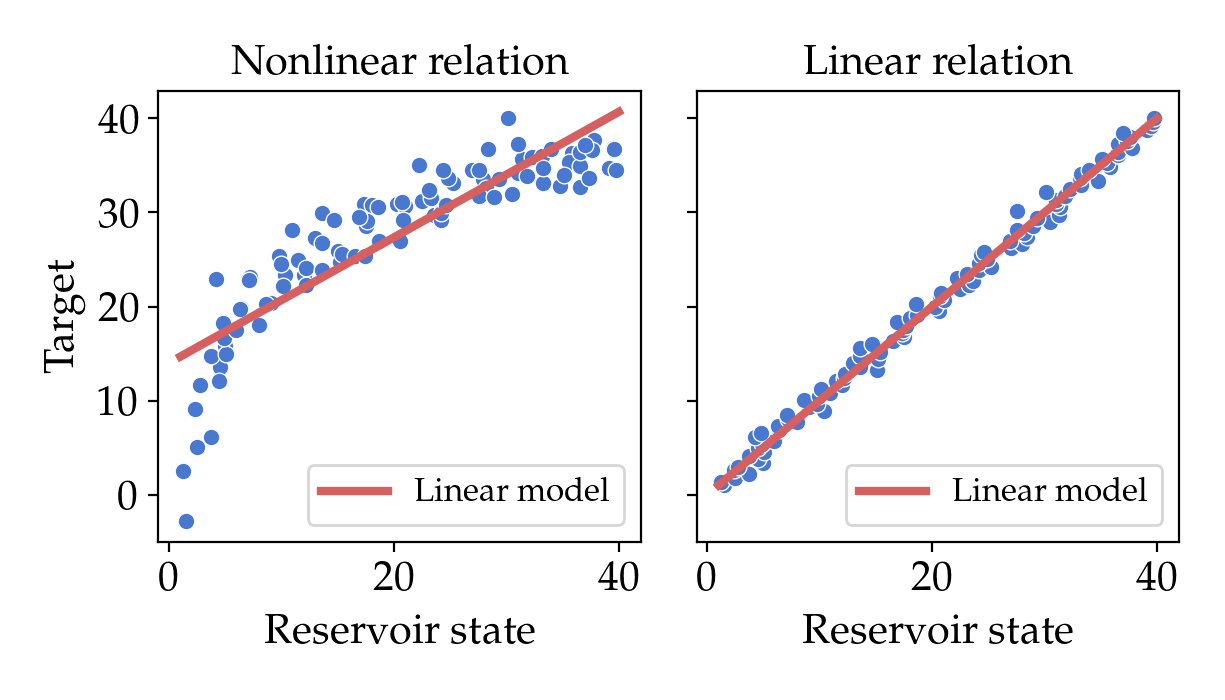
\includegraphics[height=5.7cm,keepaspectratio]{img/explainer_input_sep.png}
        \caption{ }
        \label{fig:input_sep_principle}
    \end{subfigure}
    \caption[Demonstration of the Echo State Property and illustration of linear input separation.]{
        Demonstration of the Echo State Property and illustration of linear input separation.
        (\subref{fig:fading_mem_principle}) Demonstration of the \acrlong{esp} in an ESN with 100 nodes, leak rate 0.16 and spectral radius 1.25. The ESN is subjected to the same input sequence, with two different initial state vectors. The plot shows the activation value of the same node through time.
        (\subref{fig:input_sep_principle}) Example of linear input separation between a target task and the reservoir state. The left plot shows a nonlinear relation (in this case, logarithmic). The right plot shows a linear relation. The red line shows a linear regression model fitted to the data.
    }
    \label{fig:prc_principles}
\end{figure}



\section{Time Scale of Reservoir Dynamics} \label{section:rc-time-scales}

% Reservoirs can have a wide range of time scales
As Section \ref{section:rc} already stated, reservoir computing occurs inherently in the time domain.
That means we must carefully consider the time scale at which the reservoir dynamics occur.
The time scale of reservoir dynamics can vary significantly. 
For example, imagine a physical reservoir implemented as a resistive-capacitive electrical network. 
The time it takes for the network to reach a resting state can be changed by increasing or decreasing the resistance and capacitance of the elements present in the network.
We can tune the dynamics' time scale to range from milliseconds to minutes or hours.


% Effect of time scale on memory capacity
A faster time scale also means the reservoir returns to its resting state faster, decreasing the system's memory capacity. Figure \ref{fig:leak_rate_verstraeten} from \citet{verstraeten_towards_2009} illustrates the effect of time scale on memory capacity.
The plot shows the memory capacity for ESNs with twenty nodes and different leak rates. The smaller the leak rate, the wider but flatter the memory curve becomes.
That means that networks with a lower leak rate show better long-term memory at the cost of precision in memory of more recent inputs.

\begin{figure}[]
	\centering
    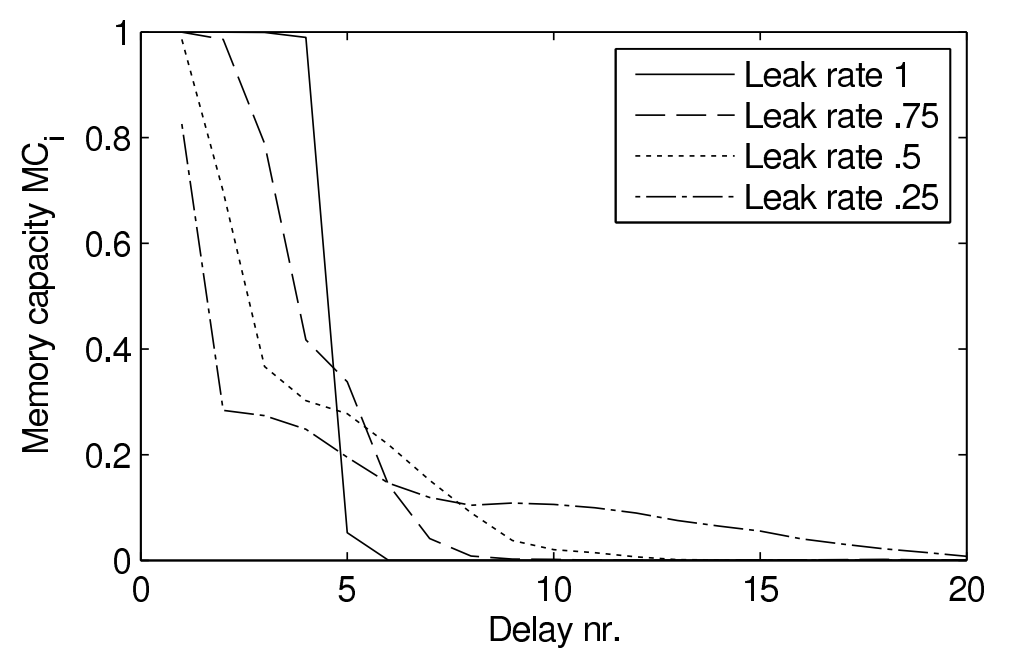
\includegraphics[width=0.55\textwidth]{img/leak_rate_verstraeten.png}
	
	\caption[Memory capacity for \acrshort{esn}s with different leak rates (from \citet{verstraeten_towards_2009}).]{
    		Memory capacity for \acrshort{esn}s with different leak rates (see Subsection \ref{subsection:esn}). Networks with a smaller leak rate show better long-term memory at the cost of decreased accuracy in short-term memory. This figure originally appeared in \citet{verstraeten_towards_2009}.
        }
	\label{fig:leak_rate_verstraeten}
\end{figure}


% This is shown in Figure 3.2. In this plot, the memory curve for a reservoir of 20 tanh nodes
% is shown with dierent leak rates. The plot shows that decreasing leak
% rates cause the memory curve to become flatter and wider. This means
% that the reservoir has worse memory of recent inputs, but better memory of inputs further in the past. Thus, by decreasing the leak rate we
% increase the longer-term memory of the nodes at the expense of precision
% in recalling the more recent inputs.


% Takeaway for reservoir computing
The takeaway here is that the time scale of the reservoir dynamics plays a vital role in its ability to solve a given task. 
A reservoir highly synchronized to its inputs will display faster dynamics and thus a shorter but greater precision integration window for solving tasks.
Conversely, a reservoir with higher memory capacity will typically exhibit slower dynamics and thus a longer integration window, at the expense of short-term precision.


\subsection{Sampling of a Continuous-Time Reservoir}

% What is the problem when sampling a continuous-time signal?
While the dynamics of a physical reservoir operate in continuous time, most applications implement the readout model digitally using a conventional computer and sensors that discretely sample the input signals and reservoir state.
According to the Shannon-Nyquist sampling theorem, to sample a continuous signal without losing information we must sample at twice the rate of the largest frequency component present in that signal \citep{shannon_communication_1949}.
Hence, determining the right time scale at which the desired reservoir dynamics occur plays a prominent role in PRC system design. 
Undersampling critical signals in the reservoir will result in information loss by introducing aliasing in the sampled signal. 
In conclusion, effectively sampling the reservoir state presents an additional optimization problem when implementing RC with physical reservoirs.


% What are the problems with undersampling or oversampling?
% Sampling at a higher frequency than the reservoir dynamics that can solve the desired task adds high-frequency noise to the signal. 
% The presence of this additive noise can degrade the performance of the linear readout function. 


% - TODO: Maybe here I can add a figure that is a toy demonstration of under and oversampling in an RC system?

 

\section{Evaluating Reservoir Performance} \label{section:reservoir-eval}

% Introduction to the different properties of a reservoir to be benchmarked.
Before attempting to solve a specific computational task, it is important to 
map out what the physical reservoir can do by benchmarking its computational properties.
To have computational capacity, a reservoir should show input separability and fading memory \citep{nakajima_information_2015}.
Evaluating these properties is in fact a way of characterizing the echo response function of the system as described in Section \ref{section:rc-general}.
% To determine the computational capacity of a reservoir, we must evaluate it on three key fronts: (i) input separability; (ii) fading memory property; (iii) memory capacity \citep{nakajima_information_2015, nakajima_physical_2020}.

% Q: add (iv) stationarity?

\subsection{Input Separability}

% What is input separability
The readout function is a strictly linear model. 
To solve nonlinear tasks, the reservoir must transform its inputs such that the task becomes a linear function of the reservoir state.
In other words, there must be a linear relation between the reservoir's observable state and the target task.
Figure \ref{fig:input_sep_principle} shows an example of linear input separation in a reservoir.

However, the nonlinear transformation applied by a finite reservoir cannot solve any arbitrary task.
In addition, the presence of notable recurrent effects in the reservoir may degrade precision in recalling recent inputs (Section \ref{section:rc-time-scales} explores this phenomenon further).
When the input transformation applied by the reservoir results in an observable state from which a readout function can compute the desired task efficiently, we speak of good input separability.
Good input separability is a function of both nonlinearity and memory, and the optimal mix of both properties varies depending on the task.


% How to measure input separability
One way to evaluate the input separation of a reservoir relative to a given task is to train a reservoir readout and a control readout model \citep{ushio_computational_2021}. 
The former fits to the reservoir state, while the latter fits to the environmental signals directly.
If the expanded state of the reservoir contains helpful input separation for the task, the reservoir readout will perform better than the control model.


\subsection{Fading Memory} \label{sec:fading_memory}

% Introduction to fading memory
Section \ref{section:esp} already stated the importance of fading memory in physical reservoirs.
However, this property is difficult to measure directly.
Nonetheless, we will outline two ideas for measuring this property in physical systems.


% Method 1: warmup time
The first method attempts to measure the warmup time of the reservoir. 
The idea is simple: initialize the same reservoir with different starting conditions, then measure the time it takes for the reservoir state to synchronize to the input.
If the physical system displays the fading memory property, then the trajectories of the reservoirs will eventually synchronize, even if initialized with different starting conditions.
Figure \ref{fig:memory_esn_start} demonstrates this method on an \acrshort{esn} with different leak rates. 
In this experiment, An \acrshort{esn} is subjected to identical input series with two different initial reservoir states $\mathbf{x}$.
The rate at which the reservoir syncs to the input signal depends on the time scale of the reservoir dynamics dictated by the leak rate.

% Method 2: signal spike
In the second method, we subject two reservoirs to identical input signals. 
One reservoir will serve as the test subject, while the other acts as a control.
After the two systems have synchronized to the input, we briefly apply an environmental impulse to the test reservoir, after which the original input signal resumes.
We then measure the time for the test reservoir to resynchronize with the control reservoir.
This impulse can look different depending on the type of reservoir. 
For example, we can temporarily remove the reservoir from its environment such that it no longer receives any environmental stimuli.
Another possibility is to apply an unexpected and artificial stimulus for a short time.
Regardless of how we realize the impulse, we must apply it long enough to have a noticeable impact on the trajectory of the reservoir dynamics.
Otherwise, it is impossible to measure the time until the reservoir synchronizes to the regular inputs.
Figure \ref{fig:memory_esn_impulse} demonstrates this method on an \acrshort{esn}.
This time, all input values between time steps 60 and 80 are set to a fixed value of ten times the standard deviation of the input signal.
After step 80, the reservoir gradually returns to its original behavior, at a rate proportional to its leak rate.


% Measuring divergence in trajectories
Both methods rely on measuring the divergence in behavior of a reservoir when subjected to different conditions. 
To quantitatively compare the difference between reservoir states at time $t$, we can use a distance metric such as \acrfull{mse} on its observable state $X$:

\begin{equation} \label{eq:MSE}
    \text{MSE}(t) = \frac{1}{N} \sum_{i=1}^{N} \left( X_i^{(1)}(t) - X_i^{(2)}(t) \right)^{2}
\end{equation}

where $N$ is the size of the reservoir's observable state vector.


% Relation to memory capacity.
Note that in both experiments, the time it takes for the reservoirs to synchronize also informs about its recurrent dynamics and memory capacity.

\begin{figure}
    \centering
    \begin{subfigure}[b]{0.485\linewidth}
        \centering
        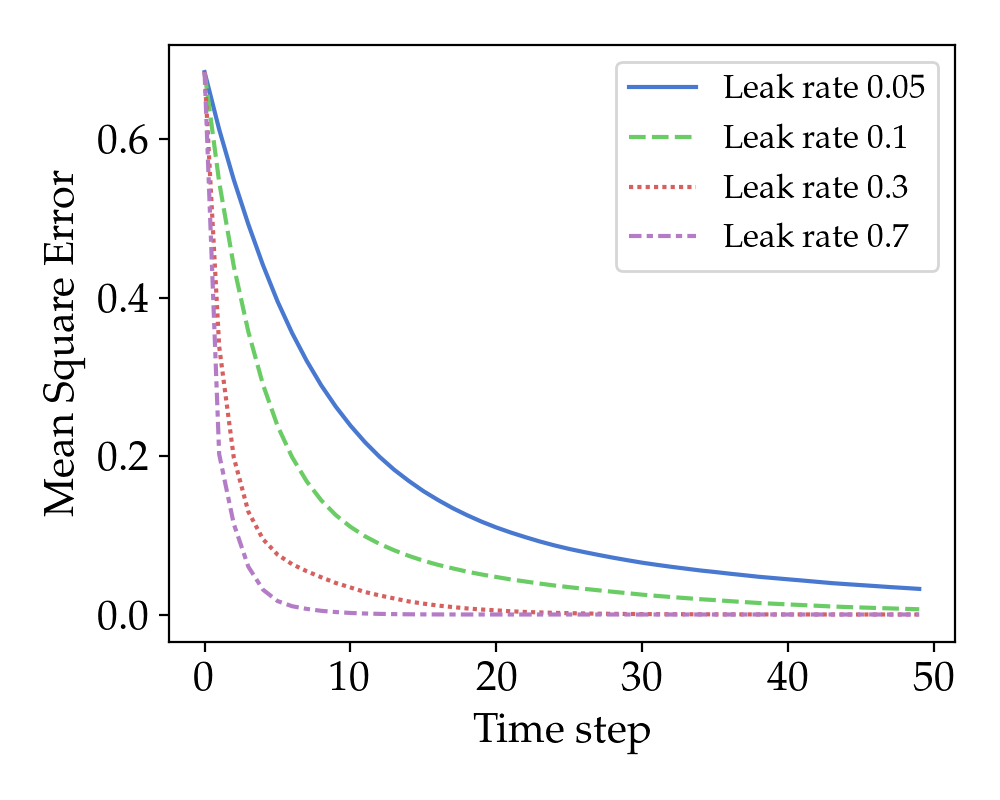
\includegraphics[width=\linewidth,height=\linewidth,keepaspectratio]{img/esn_starting_conditions.png}
        \caption{First method: divergence between reservoirs}
        \label{fig:memory_esn_start}
    \end{subfigure}
    \vskip\baselineskip
    \begin{subfigure}[b]{0.485\linewidth}
        \centering
        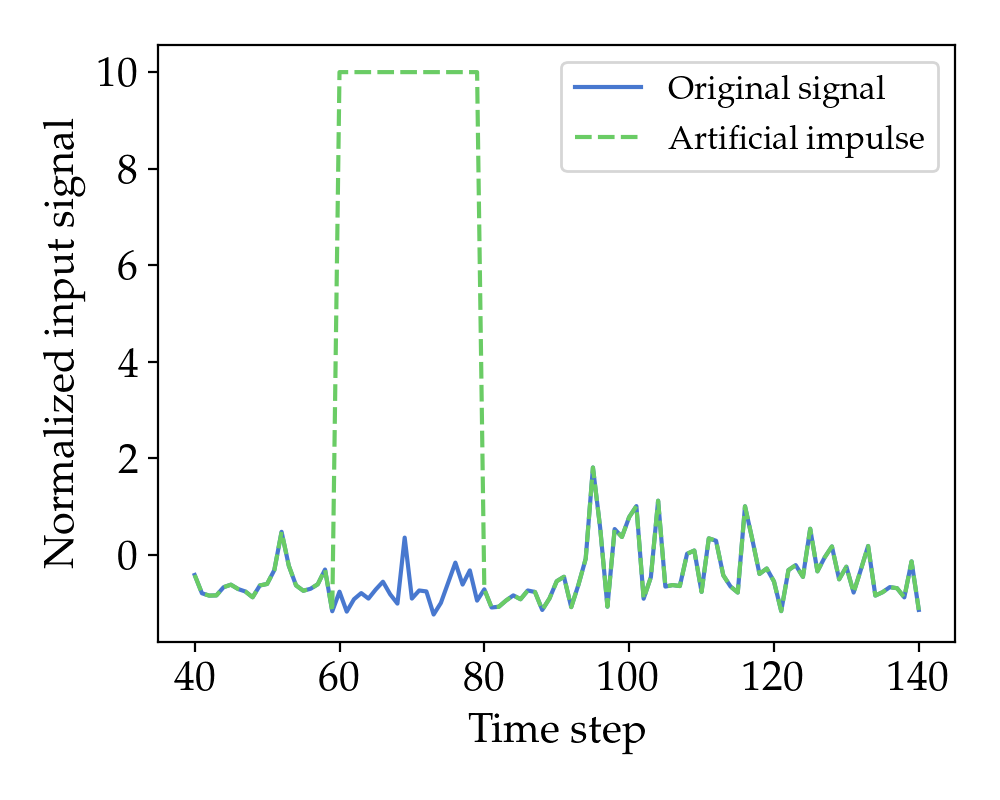
\includegraphics[width=\linewidth,height=\linewidth,keepaspectratio]{img/input_impulse.png}
        \caption{Second method: applying an artificial impulse}
        \label{fig:memory_input_impulse}
    \end{subfigure}
    \hfill
    \begin{subfigure}[b]{0.485\linewidth}
        \centering
        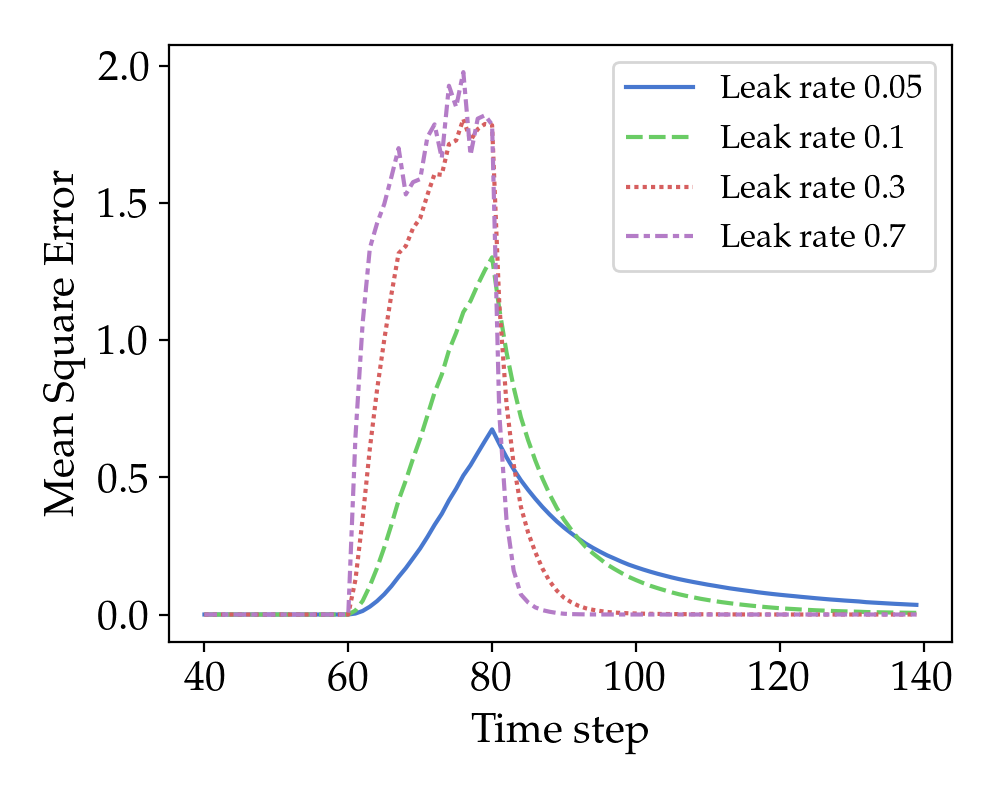
\includegraphics[width=\linewidth,height=\linewidth,keepaspectratio]{img/esn_impulse.png}
        \caption{Second method: divergence between reservoirs}
        \label{fig:memory_esn_impulse}
    \end{subfigure}
    \caption[Two methods for testing the fading memory property of a reservoir, demonstrated using a \acrshort{esn}.]{
            These figures show experimental data from testing the fading memory property of an \acrshort{esn} as described in Subsection \ref{sec:fading_memory}. 
            Both experiments use a reservoir of 100 nodes with randomly initialized weights. 
            For stability, we normalized the weights to have a spectral radius below 1.25 \citep{caluwaerts_design_2014}.
            As input data, we used the California Housing regression dataset \citep{kelley_pace_sparse_1997} which can be found in the sklearn Python package.
            (\subref{fig:memory_esn_start}) The divergence in reservoir state between two runs of the same reservoir with identical inputs and different starting state vectors. 
            The starting states are sampled from a uniform distribution between -1 and 1.
            The disparity between the reservoirs is measured by the MSE between their respective state vectors (Equation \ref{eq:MSE}).
            (\subref{fig:memory_input_impulse}) An artificial impulse with an amplitude of ten times the standard deviation of the original signal is applied between time steps 60 and 80.
            (\subref{fig:memory_esn_impulse}) The divergence in reservoir state between two runs of the same reservoir using identical starting conditions. One run receives an artificial impulse between time step 60 and 80 on all input dimensions, as depicted by Subfigure \subref{fig:memory_input_impulse}.
    }
    \label{fig:fading_memory_experiments}
\end{figure}



\subsection{Computational Benchmarks}

% NARMA
To better compare results between studies of different reservoirs, some standard benchmarks appear in the literature.
The most common \acrshort{rc} benchmark is the nonlinear autoregressive moving average (\acrshort{narma}).
We can tune the nonlinearity and memory of the \acrshort{narma} task With the $n$ parameter.
The \acrshort{narma} system is defined as:

\begin{equation} \label{prc:narma}
    y(t+1) = \alpha y(t) + \beta y(t) \left[ \sum_{i=0}^{n-1} y(t-i) \right] + \gamma x(t-n+1) x(t) + \delta
\end{equation}

where the parameters $\alpha$, $\beta$, $\gamma$, and $\delta$ are set to 0.3, 0.05, 1.5 and 0.1 \citep{nakajima_information_2015}.

For some reservoirs, it is necessary to tune the NARMA system's memory to the correct time scale to get stable results \citep{pieters_reservoir_2022}.
For this the adapted formula can be used:

\begin{equation} \label{prc:narma-timescale-adapted}
    y(t+1) = \alpha y(t) + \beta y(t) \left[ \sum_{i=0}^{n-1} y(t-\tau i) \right] + \gamma x(t-\tau n+1) x(t) + \delta
\end{equation}

where $\tau$ is tuned to the desired time scale of the NARMA system's memory.


% Delay line and polynomial expansion
We can use other simple benchmarks to evaluate the memory and nonlinear properties.
For example, predicting the past inputs of the reservoir for increasing delay tests the memory of the system:

\begin{equation} \label{prc:delay-line-benchmark}
    y(t) = x(t-\tau)
\end{equation}

where greater values of $\tau$ require more memory to solve ($\tau > 0$). 
To test reservoir nonlinearity, a simple exponentiation of the input signal can be used as the prediction target:

\begin{equation} \label{prc:polynomial-benchmark}
    y(t) = (x(t))^{n}
\end{equation}

where $n$ is greater or less than 1.


% Chaotic systems
Finally, to test a reservoir's ability to predict the trajectory of chaotic systems, \citet{ushio_computational_2021} have proposed a test using strange attractors.
In this test, a time series of a Lorenz attractor acts as the input to the reservoir.
The reservoir then has to predict near-future values of this input time series.
The test evaluates how well the reservoir can synchronize with a chaotic system, which is a common application for \acrshort{rc} \citep{tanaka_recent_2019}.


\section{Simulation of Physical Reservoirs} \label{section:prc-simulation}
If the behavior of the $\phi$-function is understood completely, it is possible to create a computer model that simulates the reservoir dynamics \citep{nakajima_physical_2020}. 
Using a simulated reservoir can have various advantages in research. 
(i) It is possible to iterate faster on designing synthetic physical reservoirs, such as FPGAs or photonic circuits, by validating designs in software before constructing the physical reservoir.
(ii) Some reservoirs operate at long time scales \citep{ushio_computational_2021}. Simulation can accelerate the research cycle by running experiments faster than in real-time.
(iii) In simulation, it is possible to operate in a highly controlled environment, which makes it possible to solve a constrained version of a problem first. 
For example, it is possible to dictate identical initial conditions in every experiment run or enforce static reservoir dynamics where the physical counterpart may experience some malleability caused by the environment.

\section{Summary} \label{section:prc-summary}

This chapter showed how physical reservoir computing outsources computation to physical dynamical systems.
This works thanks to the emergent computational qualities present in nonlinear dynamical behavior.
A simple linear readout function is used to transform the reservoir's state into a useful output.
In computer models, we can observe the reservoir state directly.
In physical implementations, we observe the reservoir using sensor data.

To perform useful computations, the reservoir must perform the suitable nonlinear transformations and convolutions to its inputs such that the problem becomes linear.
Another condition for \acrshort{prc} is a fading memory of past inputs; Fading memory is essential to performing deterministic computations.

To test whether a physical material is suitable for reservoir computing, we can design a suite of regression targets to quantify the reservoir's correlation with relevant computational tasks.
In addition, we proposed two types of experiments for testing the fading memory condition: one measures the dependence on initial conditions, and the other measures the stationarity of the reservoir dynamics in time.

\chapter{Functional-structural Plant Models} \label{chapter:fspm}

This chapter looks at current developments in the field of \textit{in silico} plants, intending to design \acrshort{rc} experiments with simulated organisms.
Research with \textit{in vivo} plants is difficult and time-consuming as it involves meticulous experimental design, long observation times, and of course keeping the plants healthy during the experiment\citep{pieters_plants_2021}.
For these reasons, it is of great interest to explore computer simulations of plants that can accelerate research in reservoir computing applications.
 \label{fspm:why}

% \section{Selection criteria for RC experiments}
\section{Selecting Plant Models for RC Experiments} \label{fspm:selecting-models-for-rc}


% Types of plant models
% Plant models exist in many shapes and sizes. 
There exist many different types of plant models.
To get an idea of the various model categories one can visit \textit{Quantitative Plant}\footnote[1]{https://www.quantitative-plant.org/model. See \citet{lobet_online_2013, lobet_image_2017} for more details.}, 
a website that aggregates open-source plant models from the literature.
Listed models range from crop surface models (\acrshort{csm}) that estimate biomass and crop yield from aerial imagery \citep{tilly_multitemporal_2014} to sub-plant models that simulate gas exchange between the canopy and the environment \citep{sinoquet_ratp_2001}.

%%% TODO %%%

% Selection criteria: single organism
To select plant models for use in \acrshort{rc} experiments, they must meet certain criteria. 
Firstly, the model must track the state of a single plant over time, 
as the scope of the research presented limits the interpretation of the reservoir to a single organism.
This rules out the use of e.g.\ crop surface models because they only inform about large populations of plants; in these models information on the level of an individual organism is lost (although it would certainly be interesting to apply reservoir computing principles to the ecological dynamics of a crop field).


% Selection criteria: 3d anatomy
Secondly, the plant's state should be observable from multiple fixed points of the plant's anatomy. 
These observed points must be distinct structural elements of the plant that simulate the physiological processes of a real specimen and must communicate with one another as a dynamical system.
We set this requirement because an RC system using a plant model as reservoir is intended to represent the equivalent setup in the real world.
This requirement entails a preference for mechanistic models that make few prior assumptions about plant behavior, leaving macroscopic behavior to emerge naturally from microscopic interactions at the cellular level \citep{gauthier_functional_2020}.
Ideally, the observable parameters of the plant are also empirically measurable \textit{in vivo} to enable the research results from this work to be better transferable to a real-world setting.


% Selection criteria: time resolution
Finally, the time resolution of the simulation should be sufficiently fine to observe dynamics at multiple time scales as well as avoid signal aliasing (see \mbox{Section \ref{section:rc-time-scales}}).

 

\section{Functional-structural Plant Models (FSPMs)} \label{fspm:fspm-intro}


% What are \acrshort{fspm}s?
A promising category of models that can the stated criteria is that of functional-structural plant models (\acrshort{fspm}) \citep{godin_functionalstructural_2005, louarn_two_2020}.
\acrshort{fspm} model the plant as a collection of interconnected units that represent a small structural part of the plant in space.
These units interact with the environment and with each other to simulate eco-physiological processes \citep{coussement_turgor-driven_2020}. 
The structural elements of the simulated plant form a hierarchy of interactions at different scales. Together they govern the macroscopic behavior of the organism \citep{louarn_two_2020}. Most \acrshort{fspm}s simulate interactions across a range of scales, from cell organelles to whole plant organs and even populations of multiple organisms. A schematic representation of the different scales of interactions is shown on Figure \ref{fig:fspm_scales_louarn2020}.

\begin{figure}[t]
	\centering
% 	\copyrightbox[r]{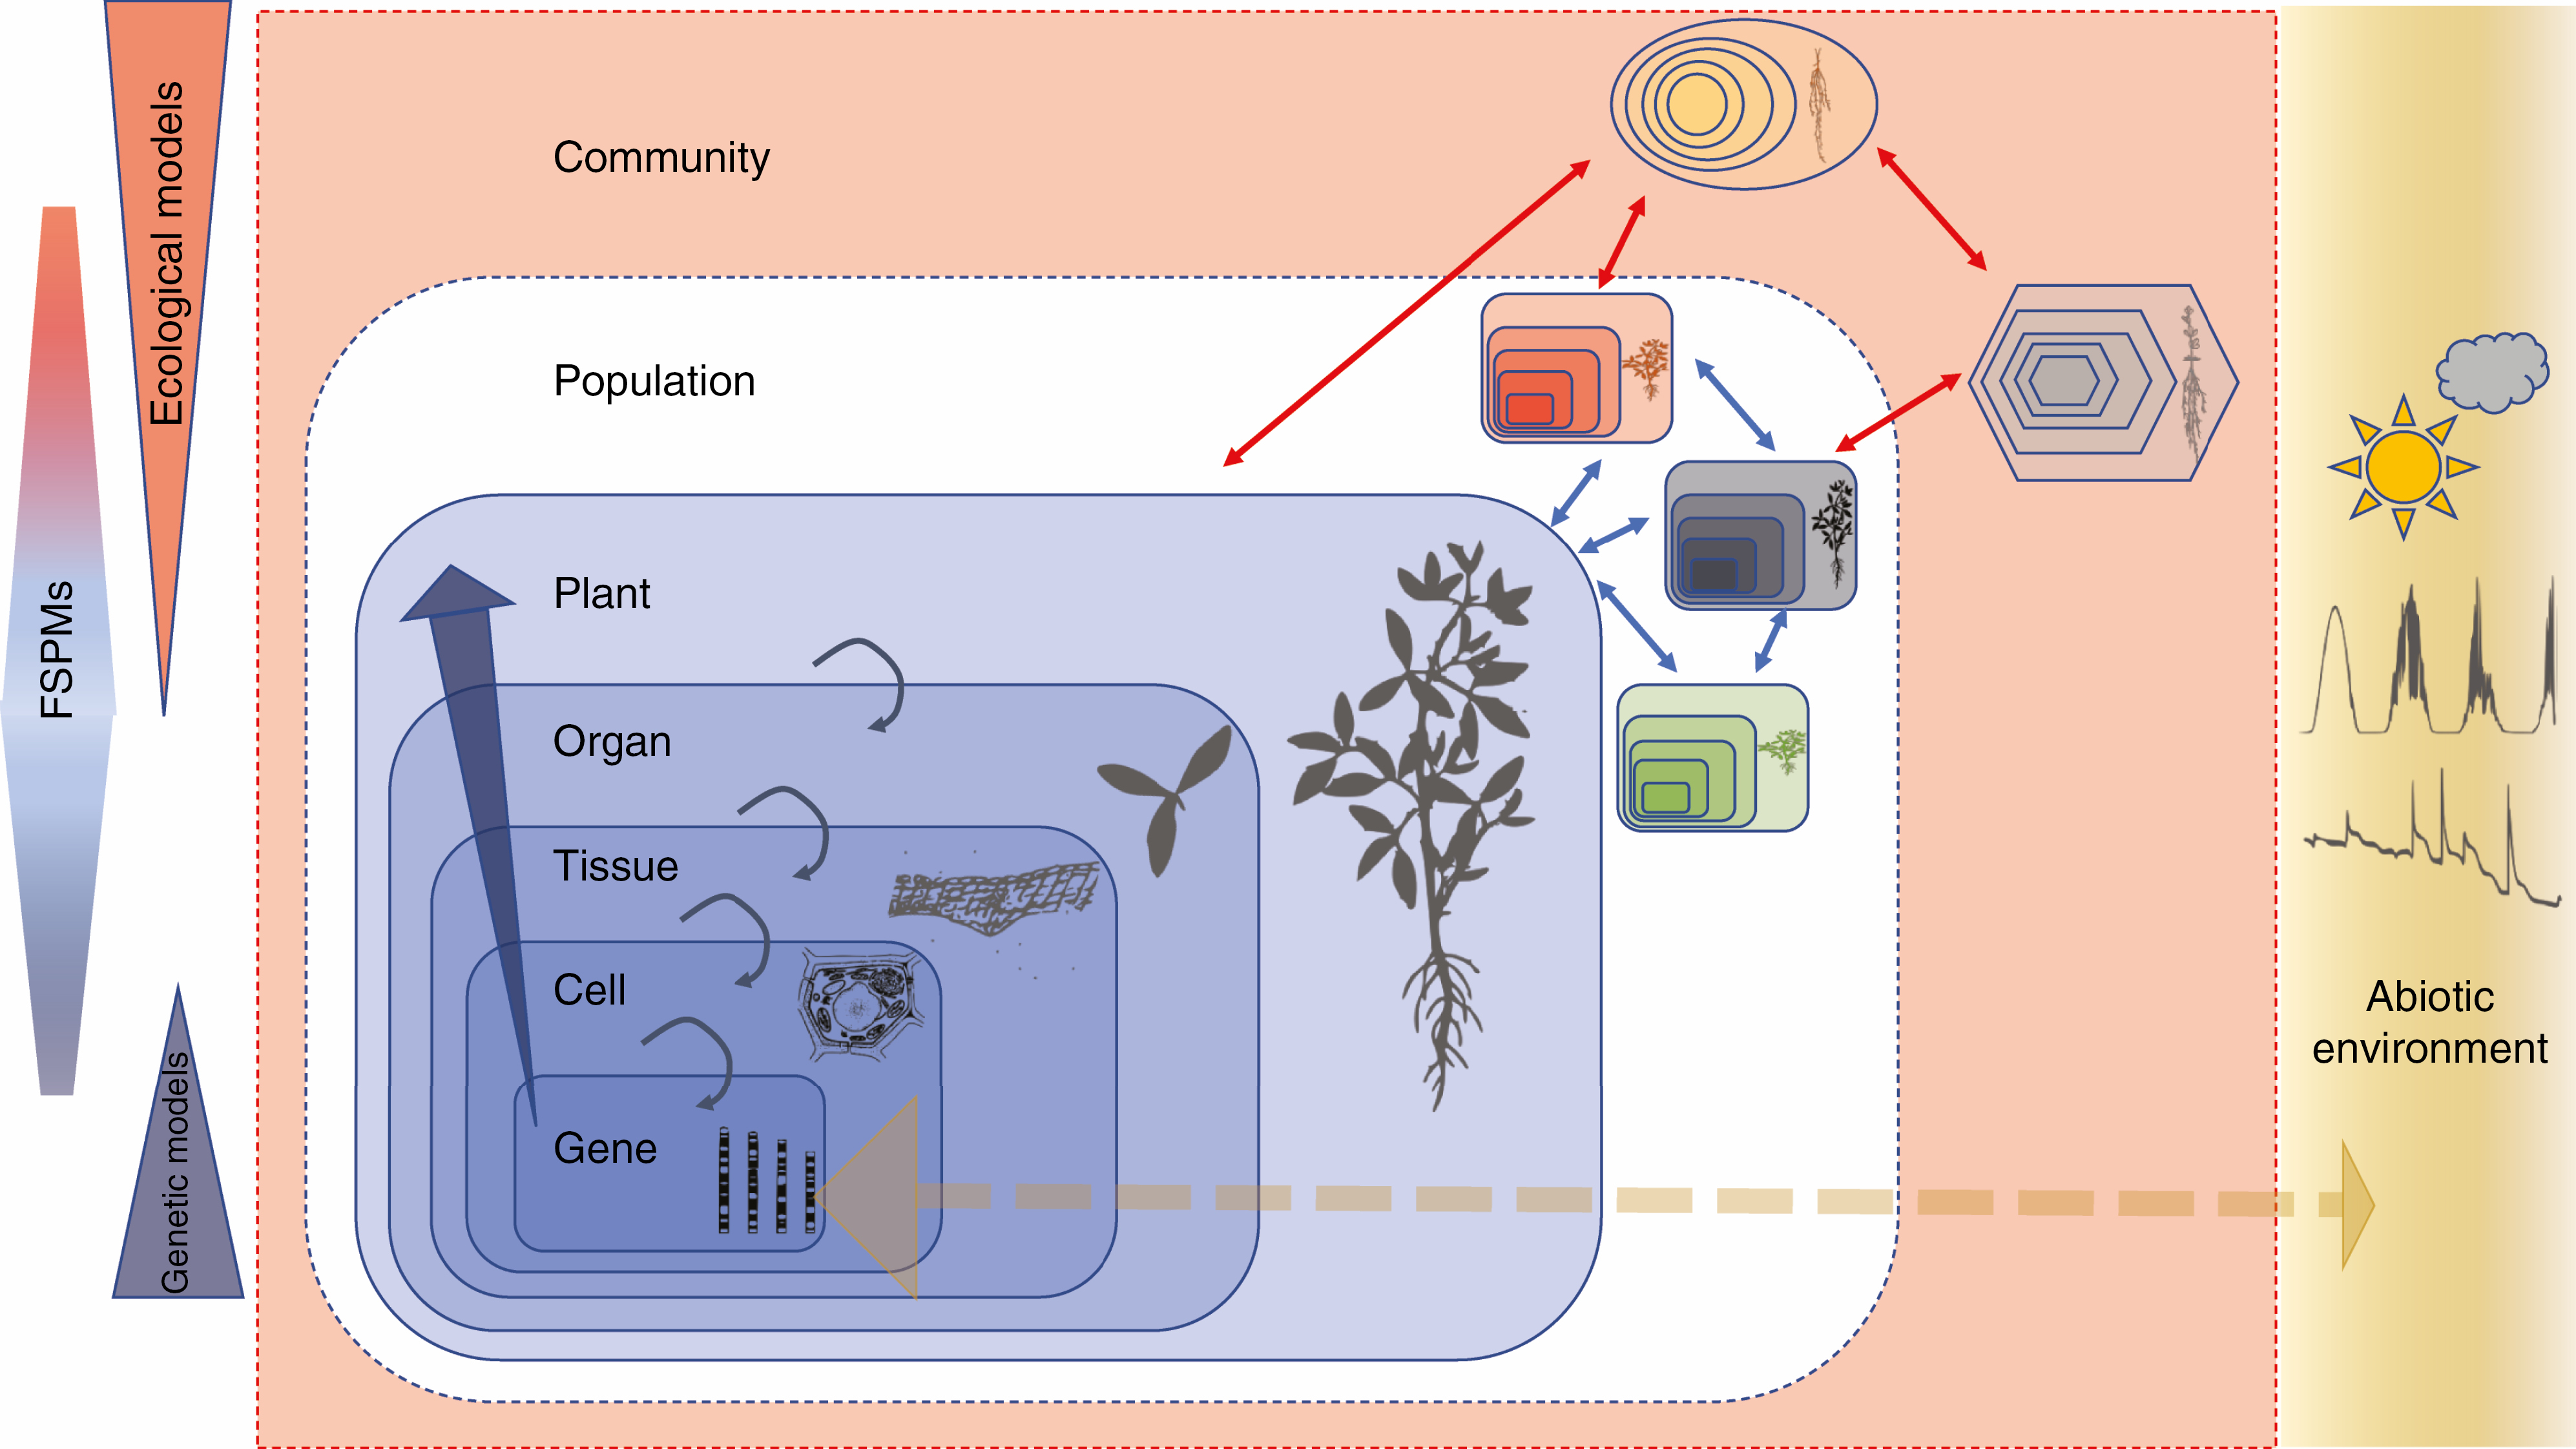
\includegraphics[width=0.8\textwidth]{img/fspm_scales_louarn_2020.jpeg}}{\textcopyright Copyright 2020 Oxford University Press}
	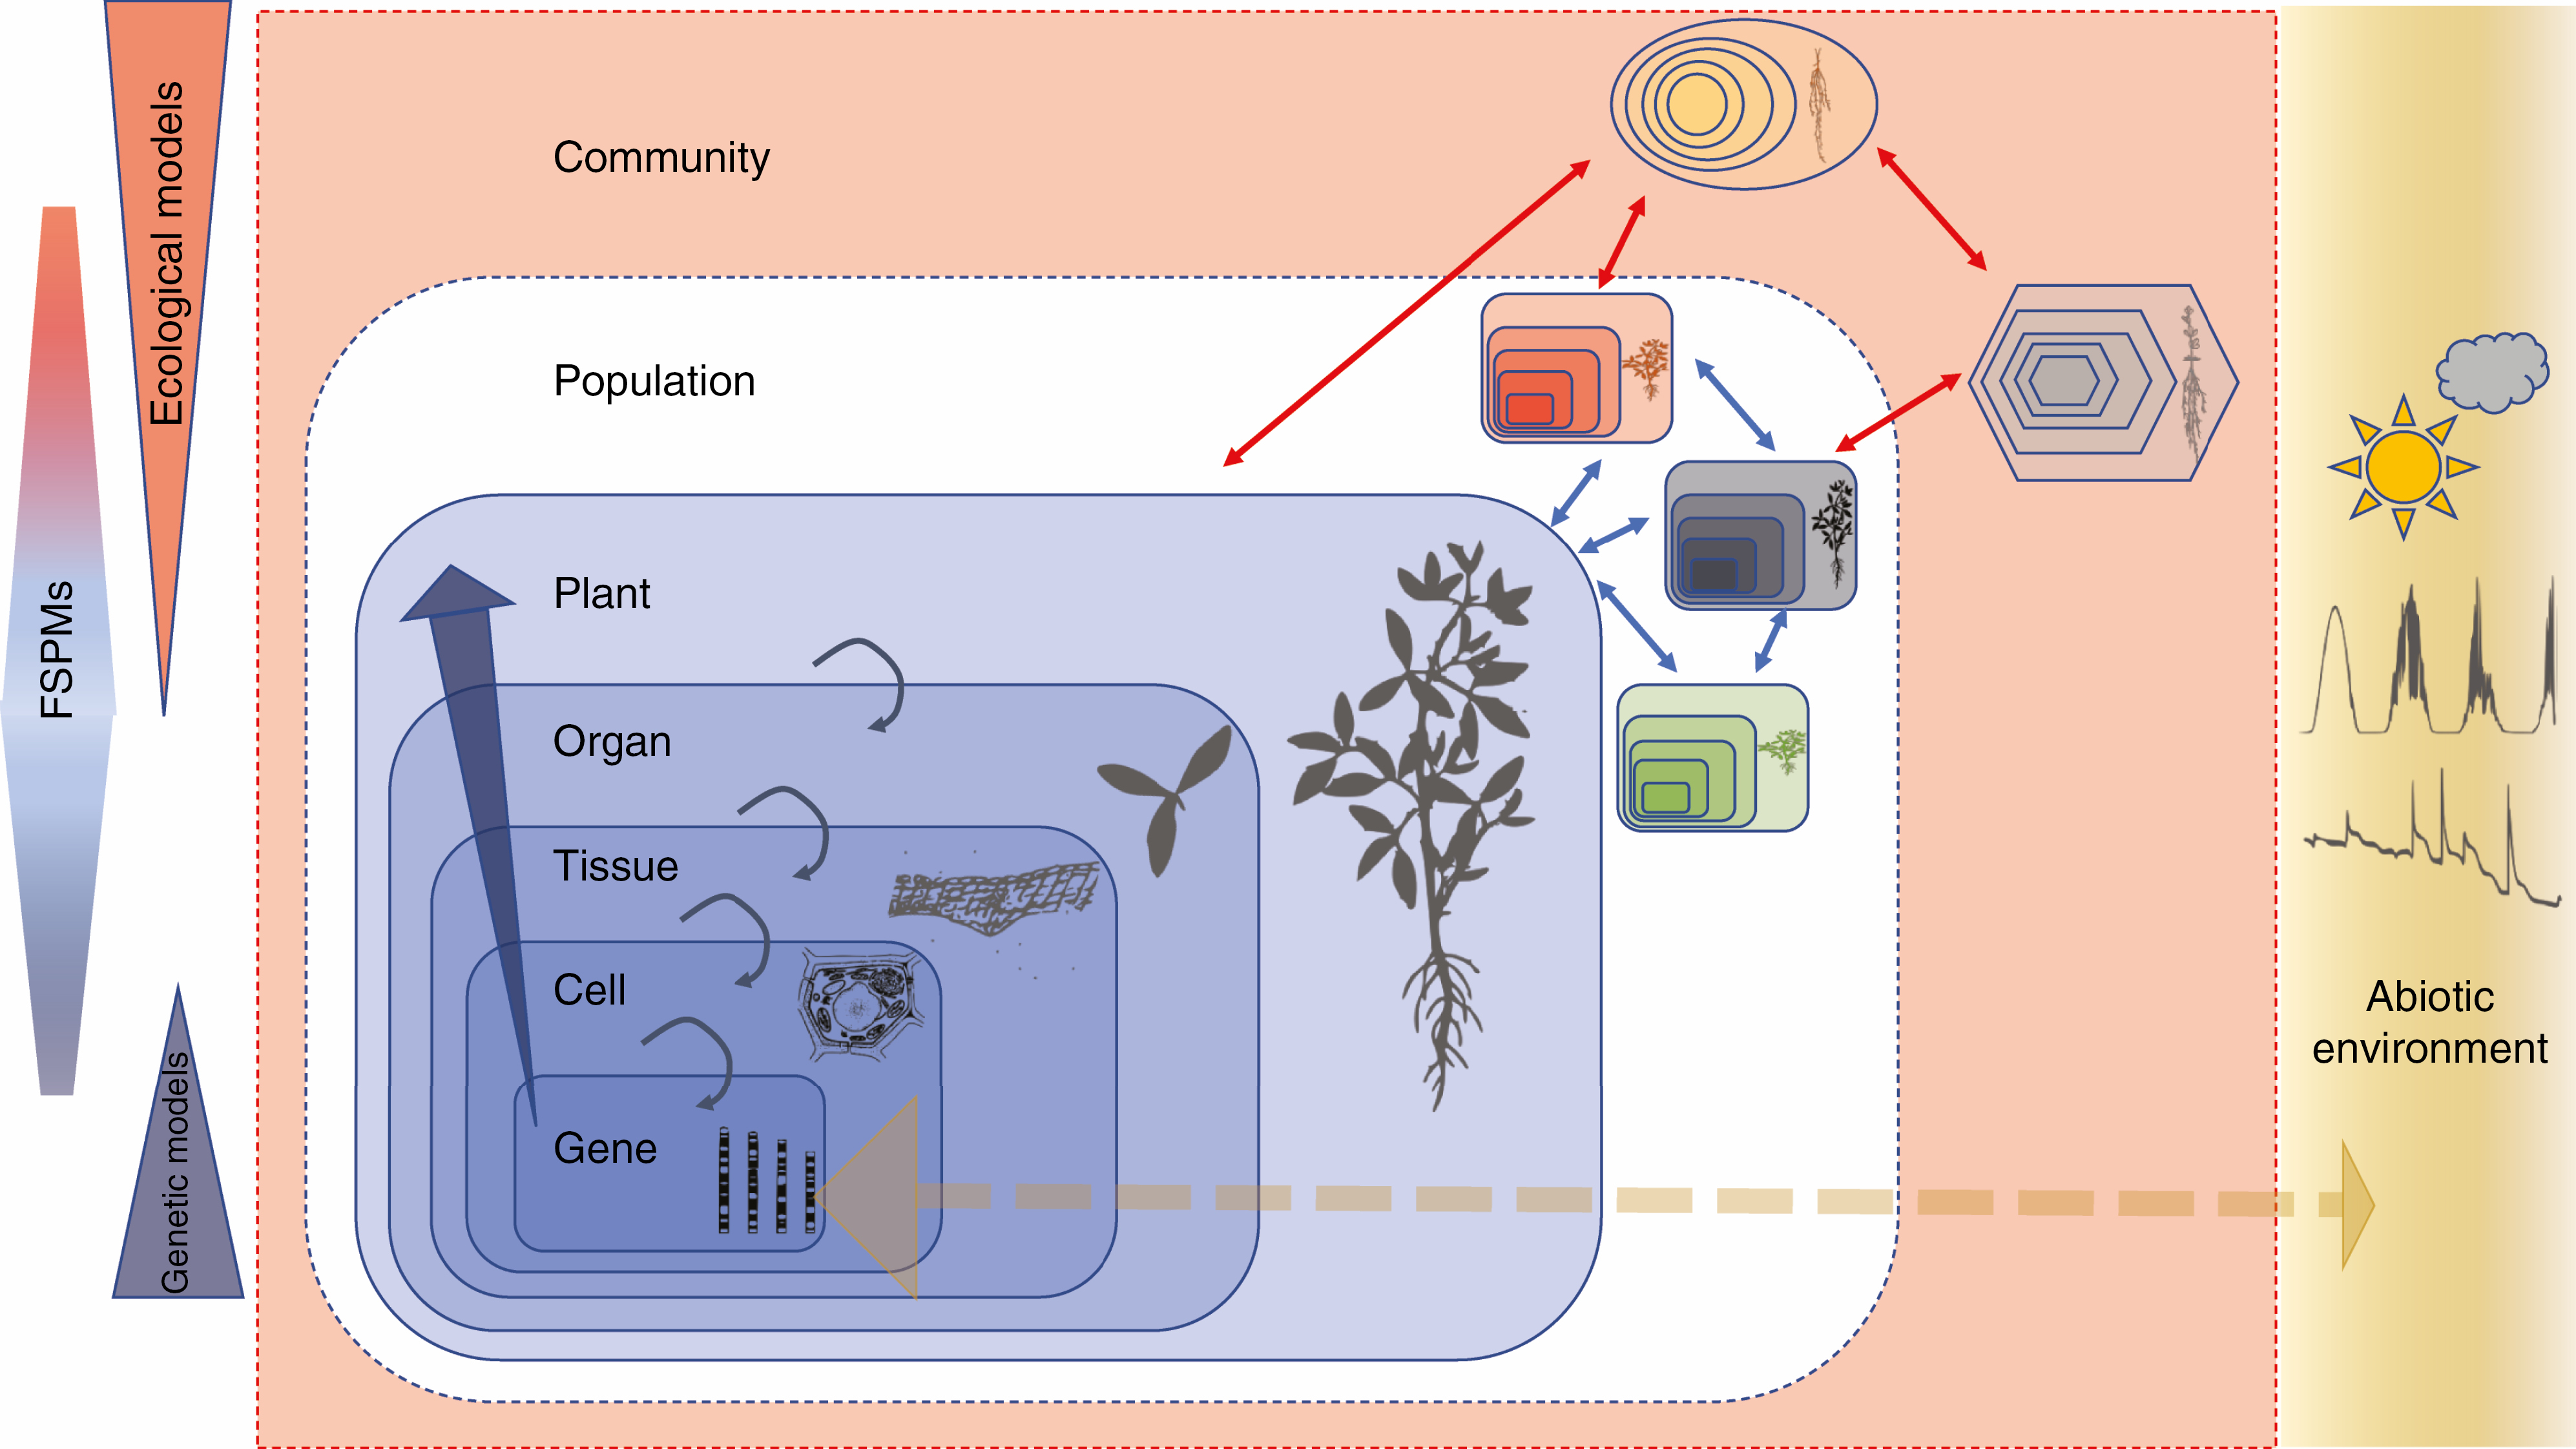
\includegraphics[width=\textwidth]{img/fspm_scales_louarn_2020.jpeg}
	
	\caption[Interactions at micro- and macroscopic scales present in functional-structural plant models (from \citet{louarn_two_2020}).]{
	        Interactions at micro- and macroscopic scales present in functional-structural plant models.
    	    \acrshort{fspm}s typically implement a subset of the scales depicted in the figure. The interactions between structural elements at one level govern the macroscopic behavior at the higher level. All levels interact with the environment. In some models, the behavior of the lowest level units is governed by variable genetic properties. This figure is reused from \citet{louarn_two_2020} with permission from the publisher.
        }
	\label{fig:fspm_scales_louarn2020}
\end{figure}


% Original caption:

% FSPMs cover a range of scale integration from gene to community level, with the focus of attention being the explanation of how plant phenotypes (centre of the figure) are built from interactions with their inner (including genetic determinants and self-regulation loops expressed at various levels) and outer (including abiotic factors and biotic interactions in plant populations and communities) environments. Interactions up to the plant scale involve sub-parts that all share the same genetic material (same shape and colour gradient in the figure) and proceed from systems biology. Interactions at higher scales integrate the interplay between entities that are genetically distinct (either from the same or different species), and contribute to predictive ecology by linking organismal traits with population and community functioning. FSPMs thus complete both classical genetic and molecular network models that are usually applied up to the cellular level, and population ecology models that are lacking a robust physiological response to environmental drivers.

% [TODO: ADD ILLUSTRATION OF FSPM]


% What are \acrshort{fspm}s for?
Functional-structural plant models owe their success to more than two decades of interdisciplinary collaboration between biology, biophysics, ecology, and computer science \citep{louarn_two_2020}.
At present, \acrshort{fspm}s have been applied in developmental biology \citep{cieslak_integrating_2016, schneider_light_2019, gauthier_functional_2020}, integrative and systems biology \citep{zhu_plants_2016, chang_systems_2019, millar_practical_2019} and applied plant sciences \citep{renton_modelling_2017, albasha_hydroshoot_2019, university_of_reading_uk_advances_2021}. 
The accelerated development in this area of research is enabled by common frameworks that standardize the description of e.g.\ plant architecture \citep{godin_multiscale_1998, boudon_l-py_2012} and eco-physiological interactions \citep{fournier_caribu_2016, zhou_cplantbox_2020}. 
Popular platforms for functional plant modelling workflows are OpenAlea \citep{pradal_openalea_2008, pradal_openalea_2015}, GroIMP \citep{vos_groimp_2007} and GreenLab \citep{de_reffye_two_2021}. 


% What do \acrshort{fspm}s model?
The precise set of simulated physiological processes varies from model to model. 
Commonly modeled factors include hydraulic pressure, water and carbon flow, and photosynthesis \citep{coussement_turgor-driven_2020, zhou_cplantbox_2020, albasha_hydroshoot_2019}. 
The complexity of the environmental simulation also differs between models, ranging from manual application of input values in root nodes \citep{zhou_cplantbox_2020} to ray-traced application of lighting conditions, including self-shading \citep{coussement_turgor-driven_2020}.
Further still, some \acrshort{fspm}s model plant growth over the span of an entire growth season \citep{lecarpentier_walter_2019, coussement_turgor-driven_2020} where others assume a static plant geometry with predefined limits for simulation duration and model accuracy \citep{albasha_hydroshoot_2019}.


% Some examples
\mbox{Figure \ref{fig:plant_model_examples}} highlights a small selection of models from the literature.
% Soybean FSPM
First, Soybean FSPM \citep{coussement_turgor-driven_2020} is a highly detailed mechanistic plant growth model. 
Soybean FSPM was developed to understand better a plant's macroscopic behavior in relation to water.
The model simulates vegetative growth driven by hydrostatic pressure inside the plant cells and incorporates a ray-traced lighting model with dynamic lighting and shading conditions \mbox{(Figure \ref{fig:fspm-soybean-fspm})}. 
% V-Mango
V-Mango \citep{boudon_v-mango_2020} models the vegatative and reproductive development of mango trees to enable \textit{in silico} experimentation with better cultivation practices.
The model allows researchers to understand why certain characteristics of mango trees make them more susceptible to pests and to study the influence of the three-dimensional tree architecture on fruit growth.
% Other models.
While this is far from an exhaustive list of what has been accomplished with FSPMs, it should give the reader an idea of what is possible with this first-principles approach to plant modeling.

\begin{figure}[t]
    \centering
    \begin{subfigure}[b]{0.48\linewidth}
        \centering
        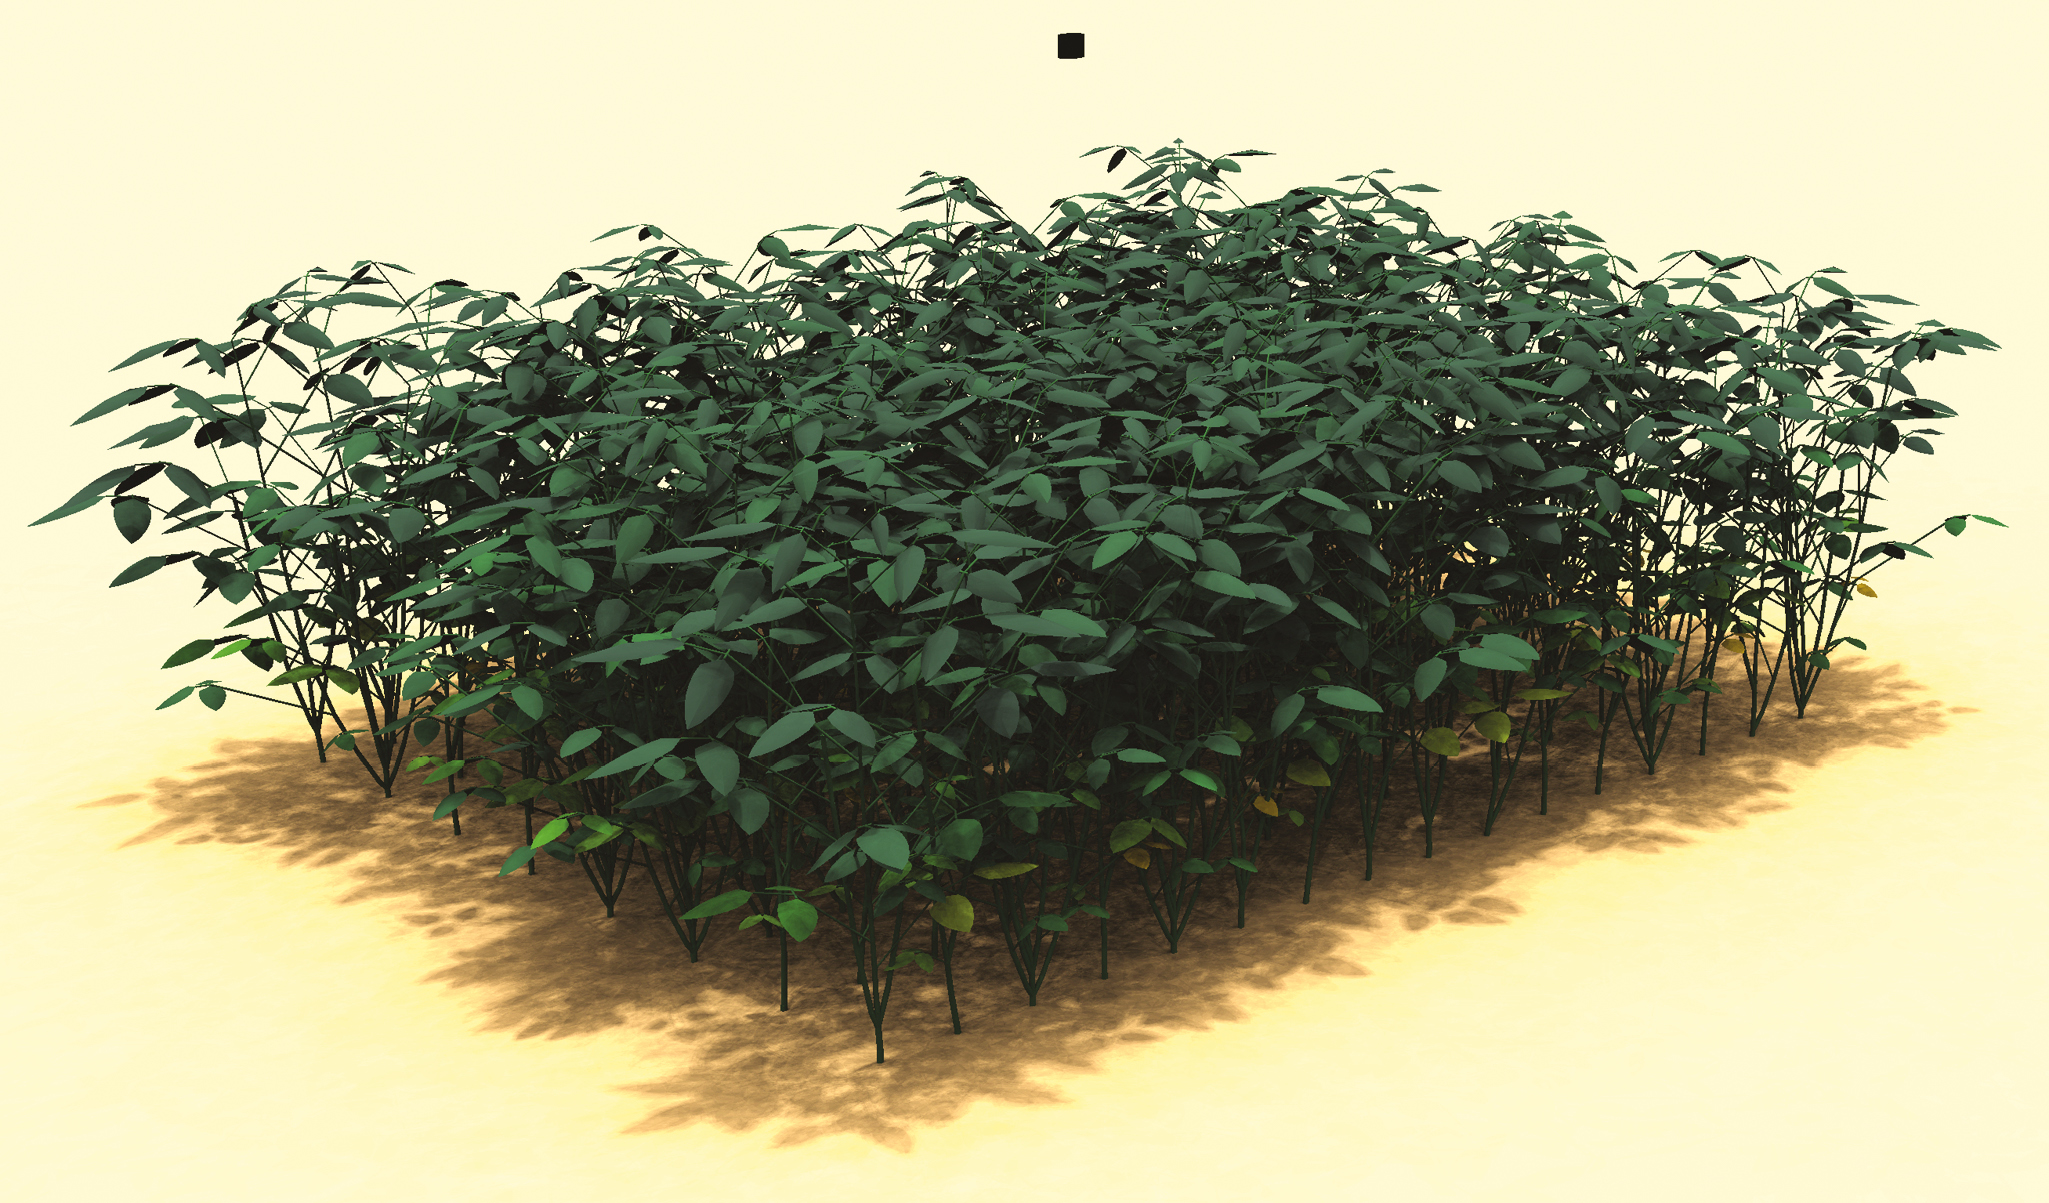
\includegraphics[width=\linewidth,height=\linewidth,keepaspectratio]{img/soybean_canopy_coussement.jpeg}
        \caption{Soybean FSPM}
        \label{fig:fspm-soybean-fspm}
    \end{subfigure}
    \hfill
    \begin{subfigure}[b]{0.48\linewidth}
        \centering
        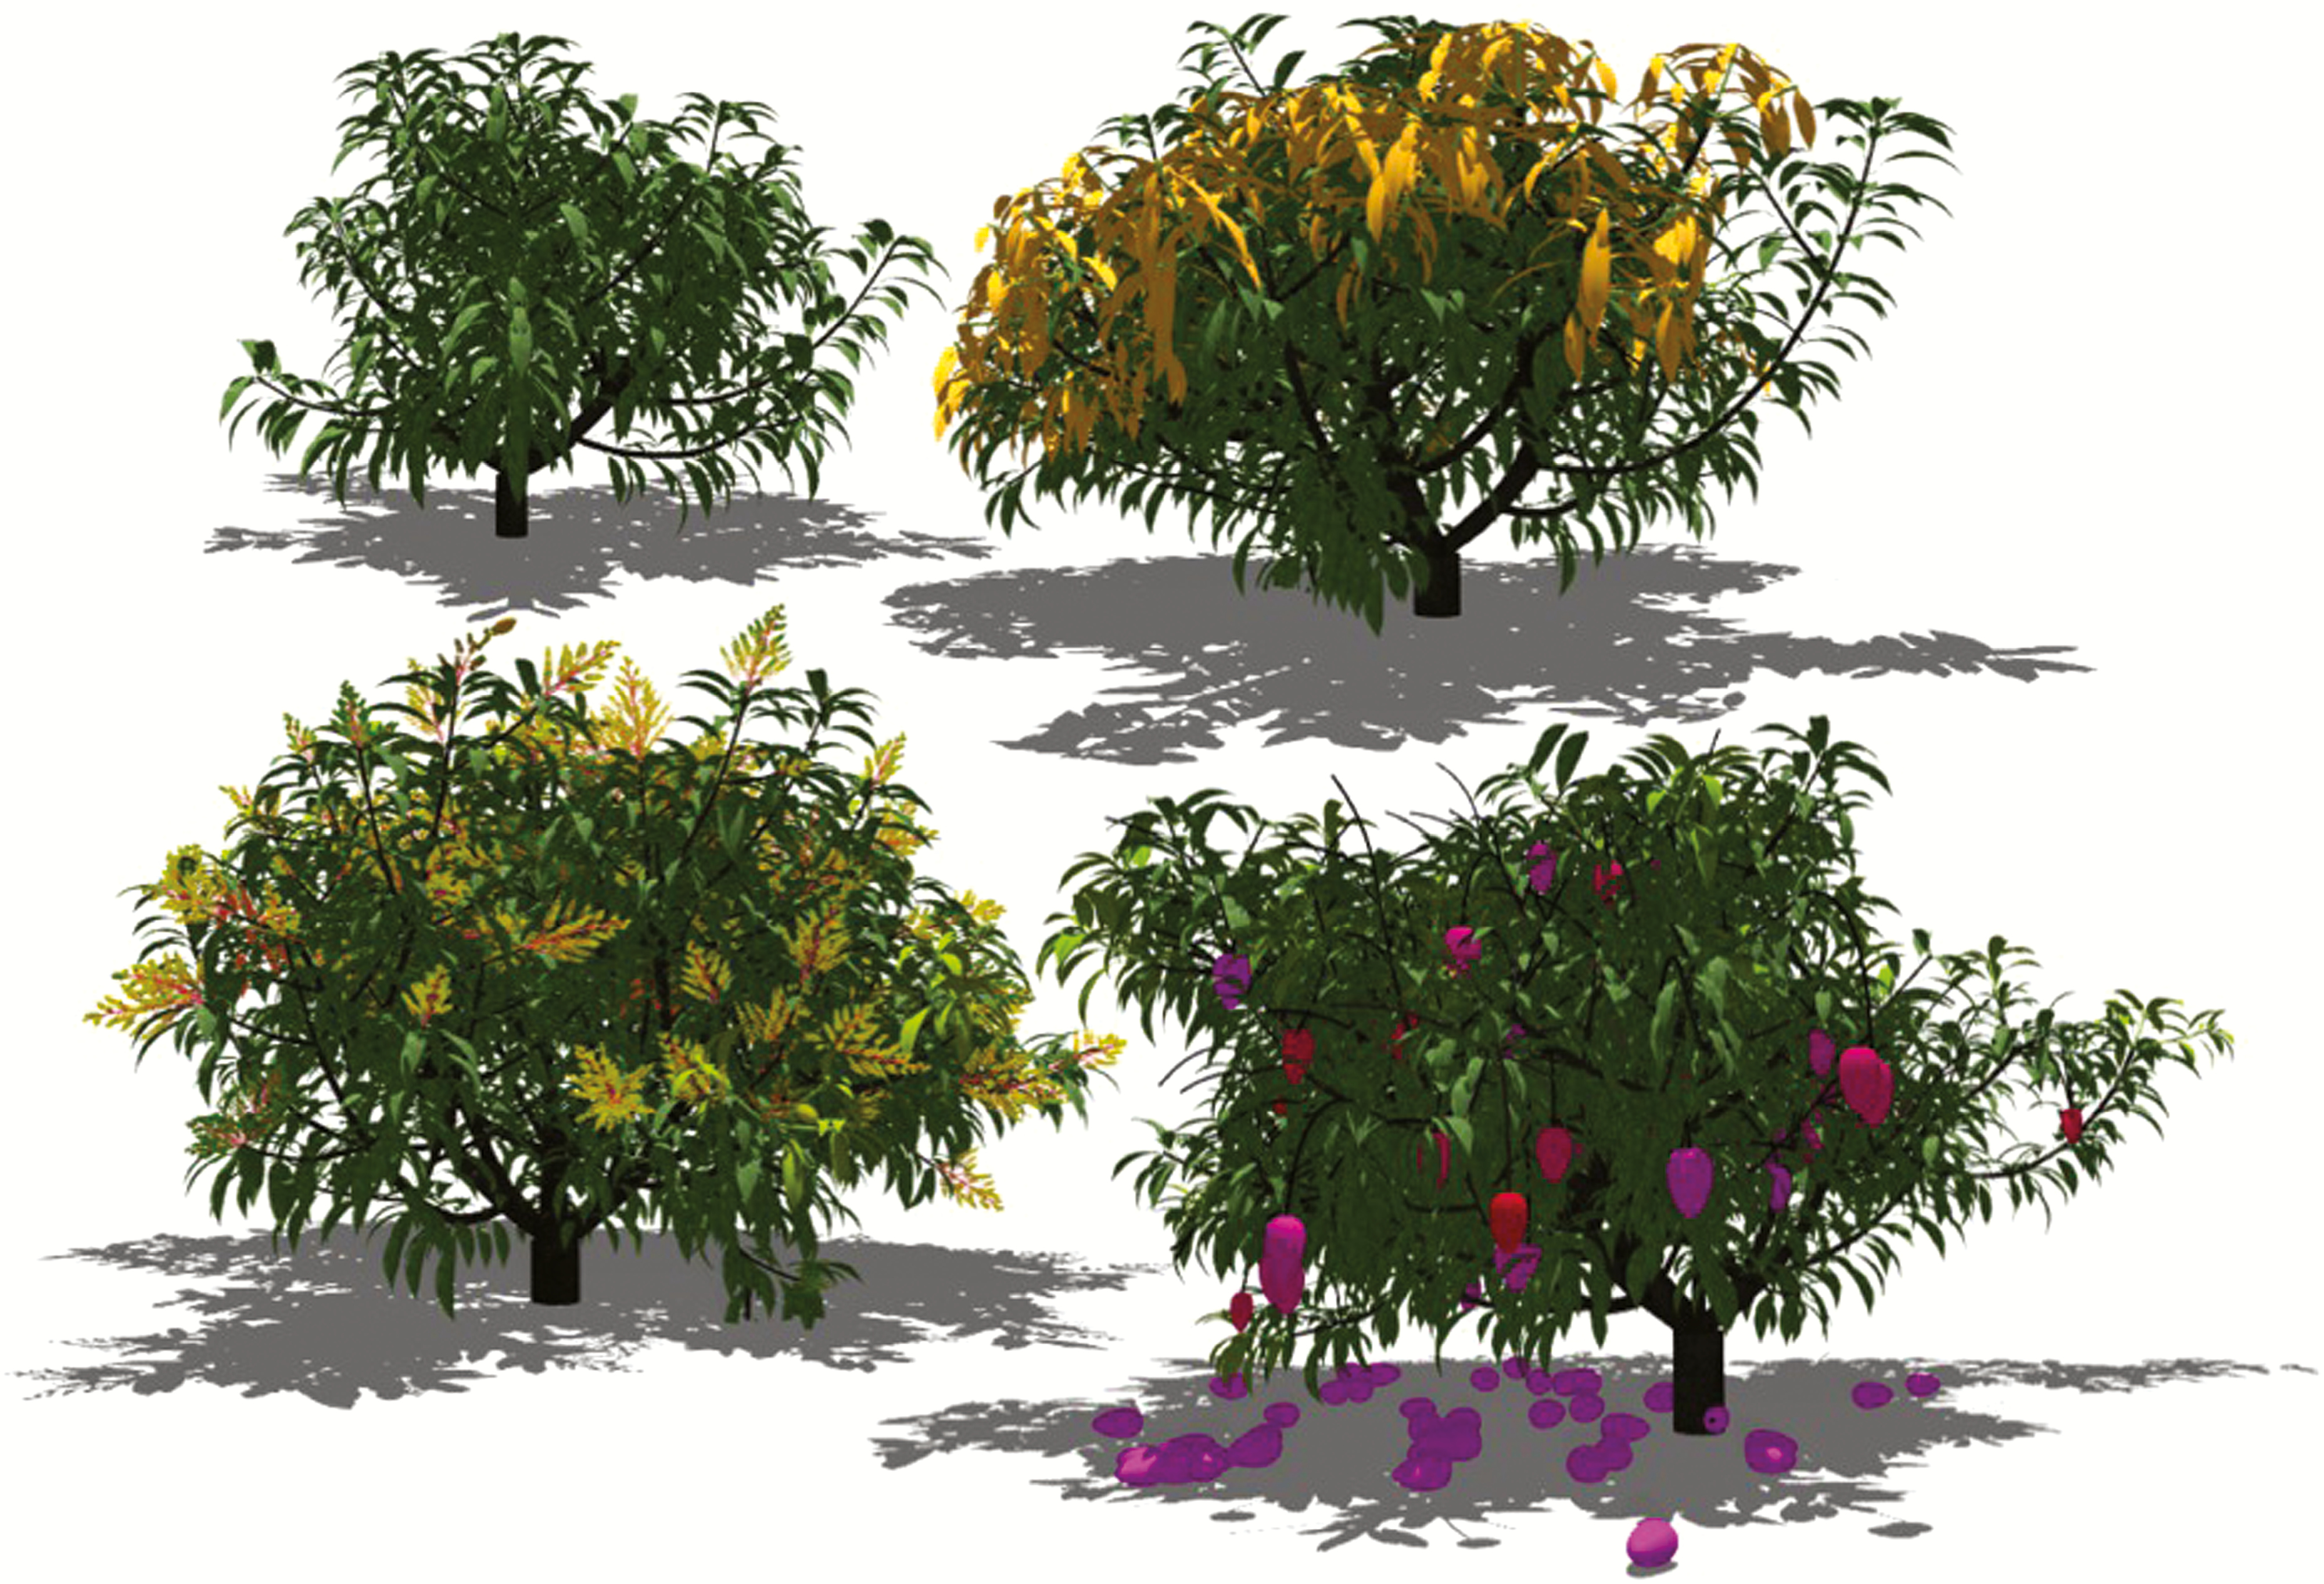
\includegraphics[width=\linewidth,height=\linewidth,keepaspectratio]{img/vmango_example.jpeg}
        \caption{V-Mango}
        \label{fig:fspm-vmango}
    \end{subfigure}
    % \vskip\baselineskip
    % \begin{subfigure}[b]{0.45\linewidth}
    %     \centering
    %     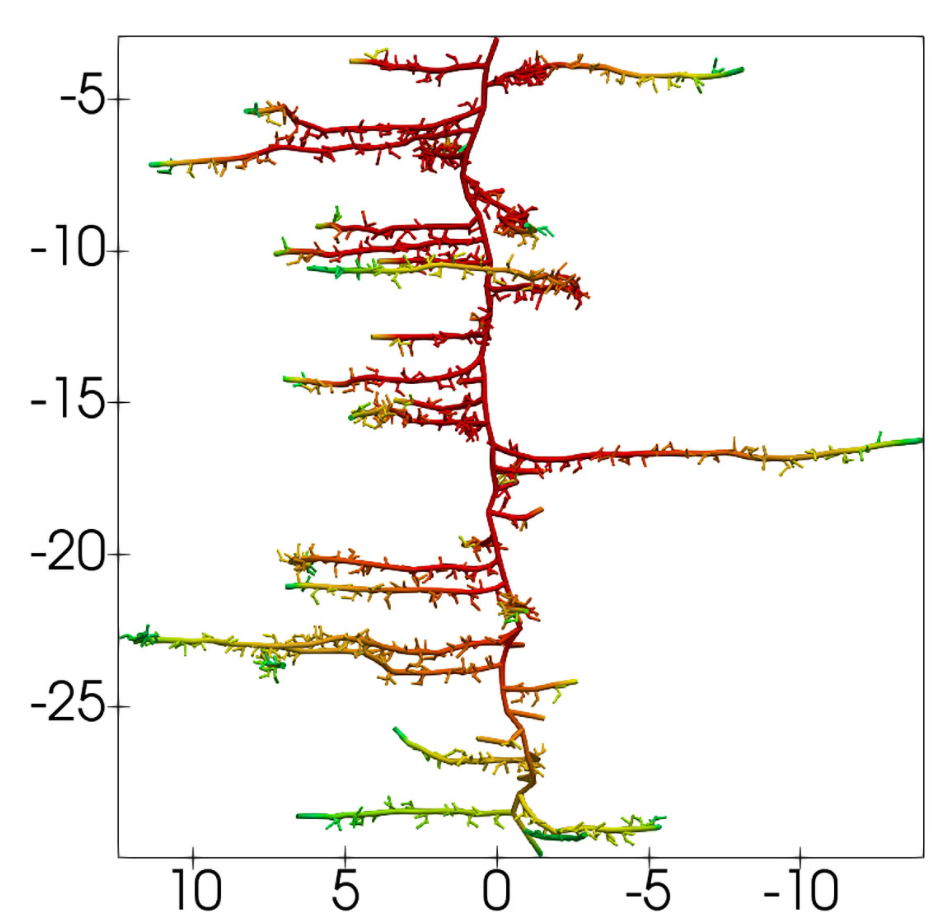
\includegraphics[width=\linewidth,height=\linewidth,keepaspectratio]{img/crootbox_example_anagallis_femina.png}
    %     \caption{CRootBox}
    %     \label{fig:fspm-crootbox}
    % \end{subfigure}
    % \hfill
    % \begin{subfigure}[b]{0.45\linewidth}
    %     \centering
    %     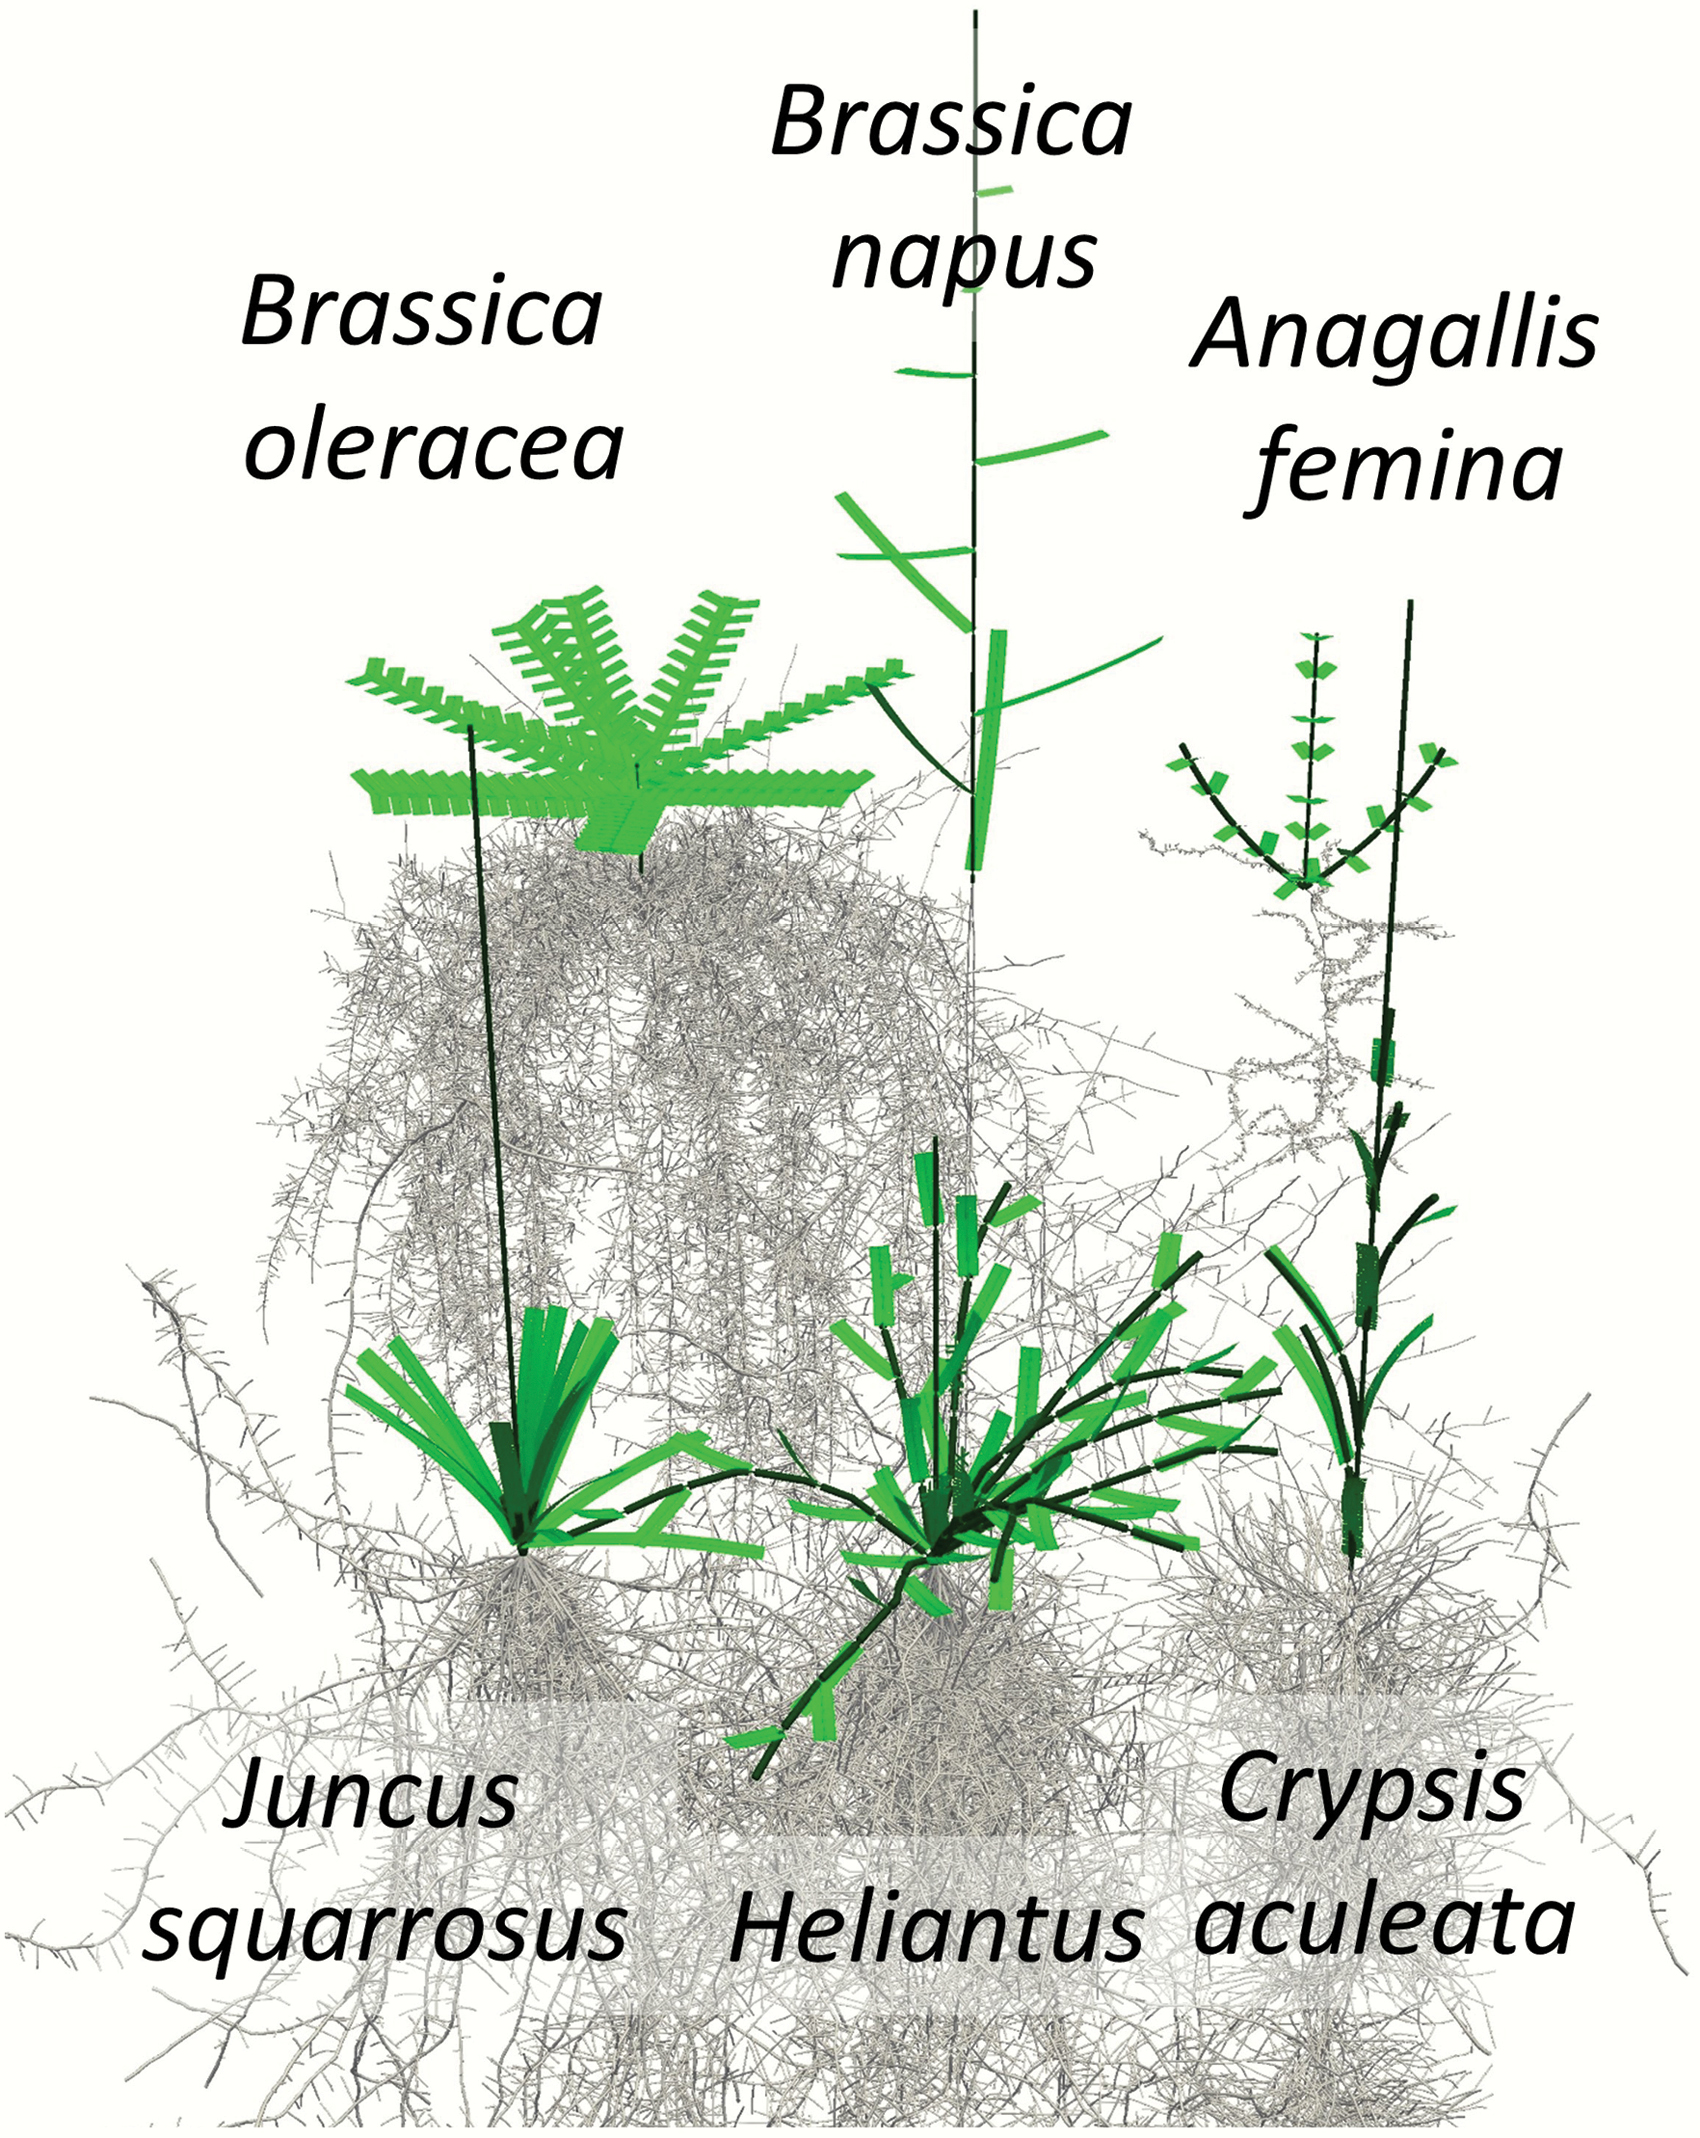
\includegraphics[width=\linewidth,height=\linewidth,keepaspectratio]{img/cplantbox_example.jpeg}
    %     \caption{CPlantBox}
    %     \label{fig:fspm-cplantbox}
    % \end{subfigure}
    \caption[Two examples of functional-structural plant models.]{
            Two examples of functional-structural plant models. 
            % (\subref{fig:fspm-soybean-fspm}) Soybean FSPM \supercite{coussement_turgor-driven_2020} is a highly detailed mechanistic plant growth model driven by hydrostatic pressure inside the plant cells. It also incorporates a ray-traced lighting model with dynamic lighting and shading conditions. 
            % (\subref{fig:fspm-vmango}) V-Mango \supercite{boudon_v-mango_2020} models the vegatative and reproductive development of mango trees to enable \textit{in silico} experimentation with better cultivation practices.
            % (\subref{fig:fspm-crootbox}) CRootBox \supercite{schnepf_crootbox_2018} is a generic framework for modeling the growth of plant roots in varying soil and environmental conditions.
            % (\subref{fig:fspm-cplantbox}) CPlantBox \supercite{zhou_cplantbox_2020} is built on top of CRootBox to provide a generic framework for modeling plant architecture and growth. It can be coupled with existing simulations of eco-physiological processes to create mechanistic plant models. 
            Figures originally appeared in their respective cited works.
            (\subref{fig:fspm-soybean-fspm}) Soybean FSPM \citep{coussement_turgor-driven_2020}. Figure reused with permission from the publisher (Copyright 2018 Oxford University Press).
            (\subref{fig:fspm-soybean-fspm}) V-Mango \citep{boudon_v-mango_2020}. Figure reused under the CC BY 4.0 license.
    }
    \label{fig:plant_model_examples}
\end{figure}

% (Coussement et al. 2018\supercite{coussement_modelling_2018})



% Caution before reusing an FSPM from the literature
An important caveat is that these models typically do not simulate a live plant as an accurate digital twin of an \textit{in vivo} plant.
Instead, they are commonly developed with a specific research question in mind and model only the physiological processes that are deemed correlated to the studied phenomenon \citep{louarn_two_2020}.
Hence, it is warranted to perform a careful comparison between the conditions and assumptions of the original study and those of a new context before reusing the model for tasks other than its original purpose.
Note that digital twin initiatives are also an active line of research. For example, researchers at WUR have been developing a digital twin system for tomato plants \citep{npec_wur_2020}.


% \section{Related work} \label{fspm:related}

% % interdisciplinary collaboration

FSPMs owe their success to more than two decades of interdisciplinary collaboration between biology, biophysics, ecology and computer science \supercite{louarn_two_2020}.


% Cite that frameworks have made it easier to iterate and build on existing work and cite some frameworks
%  	- MTG OpenAlea, LPy,  CPlantBox, GroIMP, GreenLab, 

...

% give examples of some noteable works (use [[@louarnTwoDecadesFunctional2020]] as a guide for finding good citations)

...

% Useful citations: OpenAlea platform \cite{pradal_openalea_2008, pradal_openalea_2015}, LPy for L-systems in Python \cite{boudon_l-py_2012}, CPlantBox \cite{zhou_cplantbox_2020}, GroIMP \cite{citation needed}, GreenLab \cite{de_reffye_two_2021}, ...



% \cite{balduzzi_reshaping_2017}, popular data structure MTG \cite{godin_multiscale_1998}

\section{Summary}

This chapter introduced the research field of functional-structural plant modeling, a type of model that has become the state-of-the-art in plant modeling in the past years.
FSPMs represent the plant as a 3D structure of interconnected elements, where each structural element simulates eco-physiological processes such as photosynthesis, transpiration, and water and carbon flow.
FSPMs are ideal for reservoir computing research because they model the interaction in space and time between the plant's structure and the abiotic environment.
Therefore, if plant physiology displays properties of nonlinear dynamical systems, this will be captured by a sufficiently detailed FSPM.


\part{Methodology}
\chapter{Experimental Design} \label{chapter:exp-setup}

% Introduction
 Chapter \ref{chapter:lit-prc} established the necessary background on \acrshort{rc} and explained how physical media can function as a computational resource.
Then, Chapter \ref{chapter:fspm} introduced the rich research field of functional-structural plant modeling.
Now, we present how we will identify reservoir dynamics in plants and how we can quantitatively measure the reservoir performance, using simulated plants as the experiment subject.


\section{Reservoir Dynamics in Plants}

% Introduction
To recap Chapter \ref{chapter:lit-prc}: to solve a computational problem with a physical medium, it must possess two fundamental properties.
The first is linear input separation relative to the target signal.
A reservoir can achieve this by performing a nonlinear expansion of its environmental inputs.
To perform tasks that require memory, the reservoir must also possess recurrent dynamics; 
the reservoir integrates current inputs with its memory of the past.
The second requirement is a fading memory of past inputs.
Without a fading influence of past inputs, computations carried out by the reservoir cannot consistently be reproduced.
The question remains: do plants display these properties?


% Input separation and nonlinearity
First, we consider linear input separation.
To make a target a linear function of the reservoir state, the reservoir must perform some nonlinear transformation of its inputs.
An example of this in plants is how grass responds to soil temperature. 
The growth rate of grass shows a roughly parabolical relationship with soil temperature, reaching an optimum around roughly 15-20\degree C, after which growth declines due to heat stress \citep{hurtado-uria_relationships_2013}.
This shows that a plant's behavior can show a nonlinear relation with its environment.


% Fading memory
Next, we consider the fading memory property.
Clearly, this rule does not hold for the general case; a plant temporarily subjected to extreme cold or heat will die and no longer process any information.
Favorable environmental conditions will influence the plant's growth rate, permanently altering reservoir dynamics as a function of past inputs.
Nonetheless, we might be able to identify operating ranges for specific eco-physiological processes and time scales for which the fading memory property holds up approximately.


% Reconciling dynamic reservoirs with the static reservoir assumption
In addition to the properties above, the \acrshort{prc} framework assumes the reservoir dynamics are unchanging over time.
Naturally, changing the reservoir's constitution also changes its nonlinear characteristics and memory capacity.
Plants are not stationary reservoirs in the general case because they go through several growth phases that change their structure and behavior drastically.
But here, too, we can approximate stationarity by investigating reservoir dynamics within a time window for which the growth rate is negligible.


% Conclusion
In conclusion, there is sufficient evidence to suggest that plants can display computational properties for eco-physiologically relevant tasks.
However, plant RC research is still in its infancy. It remains unexplored under which conditions the RC framework applies to plant behavior and what subset of eco-physiological processes show reservoir-like dynamics.


\subsection{Research Objectives}

% Objectives
\citet{pieters_reservoir_2022} has already demonstrated that plants can function as a medium for reservoir computing.
This work aims to expand on the foundation for plant \acrshort{rc}. 
We aim to answer the following questions:
From the subset of plant physiological processes that are empirically observable, which processes show promising input separation for eco-physiological tasks and computational benchmarks? 
And do these properties display the fading memory principle at the relevant time scale?
To answer these questions, we propose a framework for quantitatively measuring the reservoir properties of the plant's physiological functions.
This framework enables direct comparison of the reservoir performance of different physiological processes and across multiple plants.


% Why use in silico plants?
We used \acrshort{fspm}s to test this framework. 
Using simulated plant has several advantages.
It gives us the freedom to observe the plant directly, without the need for sensing technology and laboratory setups.
Consequently, it speeds up the research process and gives us a first intuition into suitable plant reservoirs. 
This can help bootstrap future \textit{in vivo} research.
In addition, we believe that \acrshort{rc} can contribute to the plant modeling community by identifying potential weaknesses in \acrshort{fspm}s.
The reason is that RC can be used for analyzing short-term as well as large scale variations; whereas current modeling efforts focuses only on long term behavior,
even though research shows that rapid physiological responses play an essential role in plant life \citep{alarcon_substantial_1994, deswaef2015a}.



\section{Framework For Measuring Plant Reservoir Dynamics}

% Introduction
In this section, we propose our framework for quantitatively measuring input separation and fading memory properties of eco-physiological processes in plants.
With these methods we will compare the capabilities of different processes.
The results will highlight which observable plant properties to pursue in future \acrshort{rc} research.


\subsection{Input Separation}

% **FIGURES:**
% - Table of regression tasks to carry out (or not)

% Introduction
First, we measure the linear input separation of the reservoir w.r.t.\ various target tasks.
We propose a collection of regression targets based on the environment and physiological state of the plant.
We choose these tasks to test the reservoir's capacity to solve biological problems.
Classification tasks are not considered because they are less relevant from an eco-physiological standpoint; 
most processes are real-valued and occur in continuous time.
We fit a simple linear readout model to the reservoir observations to test the prediction accuracy.
We then compare the predicted series against the ground truth data to compute an accuracy metric.


% Regression tasks
To paint a complete picture of the reservoir, we use a mix of target tasks.
We propose three categories of targets, previously established by \citet{pieters_reservoir_2022}: (i) environmental inputs, (ii) eco-physiological state, and (iii) computational benchmarks.
Predicting environmental inputs gives us a first indication of the plant's coupling with the environment.
For example, we can use ambient temperature, incident solar radiation or relative humidity as a prediction target.
Next, eco-physiological tasks indicate whether the observed reservoir is effective for solving biological problems.
Targets in this category can be, e.g.\ transpiration rate or photosynthesis rate on the organism level.
Finally, computational benchmarks measure a reservoir's degree of nonlinearity and memory.
We propose three targets: a delay line to measure memory capacity (\mbox{Equation \ref{prc:delay-line-benchmark}}), a polynomial expansion to measure nonlinearity (Equation \ref{prc:polynomial-benchmark}), and the NARMA benchmark to measure both properties (\mbox{Equation \ref{prc:narma-timescale-adapted}}).
Each artificial target uses an environmental series as input.
These targets are not practical tasks for a plant, but the results can help contextualize plants in the broader \acrshort{prc} literature.


% Readout model
We fit a linear readout model for every reservoir-target combination.
For the readout model we propose a simple linear regression model with a bias term:

\begin{equation}
\hat{y}[t] = \mathbf{W}^{\text{out}}\left[1;\mathbf{X}[t] \right] \label{methods:readout}
\end{equation}

To isolate the computational capacity of the reservoir from the natural correlation between the target and the environment, the environmental inputs are not fed into the readout model; the prediction relies on the reservoir only.
Model parameters \(\mathbf{W}^{\text{out}}\) are fitted to training data using ridge regression (\mbox{Equation \ref{esn:training}}).
The regularization \(\lambda\) parameter is tuned for each reservoir-target pairing. 
To find the optimal \(\lambda\), we propose a parameter sweep with logarithmic spacing, validated using cross-validation on the training data.

% Evaluation metric
We evaluate the reservoir performance on a set of held-out test data. 
Prediction accuracy is measured using the \acrfull{nmse} metric:

\begin{equation}
\text{NMSE} = \frac{1}{N} \sum_{t=1}^{N} \frac{\left(y[t] - \hat{y}[t]\right)^{2}}{\text{var}(y)} \label{methods:regression_nmse}
\end{equation}

A lower score means a more accurate prediction.
The \acrshort{nmse} has several advantages over regular \acrshort{mse} \citep{pieters_reservoir_2022}.
Because it is normalized, the results can be compared across reservoir-target pairings, including between plants.
It is also easy to interpret: a perfect predictor scores 0.0, while predicting the signal mean for every step yields a score of 1.0.


\subsection{Fading Memory}

% Introduction 
To test fading memory, we propose the impulse experiment described in Section \ref{sec:fading_memory} and illustrated in Figures \ref{fig:memory_input_impulse} and \ref{fig:memory_esn_impulse}.
The impulse can be applied to any of the environmental inputs.
The amplitude and duration of the impulse should remain within realistic boundaries so that an actual plant would not suffer permanent damage that alters the reservoir dynamics.


% Evaluation metric
To quantitatively measure the divergence $\delta(t)$ between two reservoir trajectories at a given time step, we propose a modified \acrshort{nmse} metric:

\begin{equation} \label{methods:reservoir_divergence}
    \delta(t) = \frac{1}{N} \sum_{i=1}^{N} \frac{\left( \mathbf{X}_i^{C}(t) - \mathbf{X}_i^{E}(t) \right)^{2}}{\text{var}\left( \mathbf{X}_i^{C} \right)}
\end{equation}

Where $N$ is the size of the observed reservoir, $\mathbf{X}^{C}$ the reservoir state in the control experiment, and $\mathbf{X}^{E}$ the reservoir state during the impulse experiment.
We can use a line plot of the divergence during and after the impulse to inspect the fading memory property of the reservoir.
A reservoir affected by the impulse should show a peak in divergence once the impulse is applied.
If the physiological process displays fading memory, the divergence should go down to pre-impulse levels in a finite amount of time after the artificial stimulus is removed.
Note that a substantial divergence between reservoirs subjected to the same inputs also indicates the echo state property may not hold.


\section{Considered Reservoirs} \label{sec:considered-reservoirs}

Many physiological processes inside the plant can be considered as a reservoir.
To ensure the results from this work can form the foundation for future research, we direct our attention towards those processes which are observable using existing sensing technologies.
In his doctoral dissertation, \citet{pieters_reservoir_2022} compiled comprehensive tables of physiological traits that are observable using imaging techniques (Table \ref{table:imaging-techniques}) and contact-based techniques (Table \ref{table:non-imaging-techniques}).
We can use these tables to choose which processes to look for when selecting plant models.

This work shows a preference for reservoirs observable by contactless imaging systems.
In the future, contactless systems will play a key role in scaling plant \acrshort{rc} to large arrays of plants because they do not influence reservoir dynamics and can observe multiple plants at once.
However, imaging technologies for plant RC also have some drawbacks.
They are more susceptible to noise induced by ambient factors than contact-based sensors.
Dynamic ambient factors must also be accounted for when calibrating the measurements.
Image-based systems tend to have a lower resolution, capturing less subtle variations than contact sensors \citep{pieters_reservoir_2022}.


% - Many eco-physiological processes can be considered as reservoirs. 
% - However, to keep the results of this work relevant for future research, we want to focus on processes that are observable using existing sensing technologies.
% 	- With a preference for contactless technologies; in the future we want to be able to scale PRC to larger arrays of plants on the roadmap towards practical applications in e.g. greenhouse settings.
% - In his doctoral dissertation, Pieters (2022) compiled comprehensive tables of physiological traits observable using contactless imaging techniques (table 3.1) and contact-based techniques (table 4.2).
% - For his own work he observed leaf thickness as the reservoir using leaf clips.
% 	- Leaf thickness strongly correlates with water status and turgor pressure (de swaef 2015).
% 	- However, for our own work using FSPMs, we should be able to access physiological traits directly.




\section{Summary}

This chapter proposed a framework for quantitatively measuring reservoir characteristics of plant-physiological behavior.
In the first test, we use a suite of regression targets and a standard readout model to measure the capacity to perform nonlinear tasks.
% The predicted series is compared to the ground truth using the \acrshort{nmse} metric.
The second test investigates the fading memory property in an experiment where a brief artificial stimulus is applied to the plant's environment.
% We measure how the plant dynamics restore to their original trajectory using a divergence measure based on \acrshort{nmse}.
For the considered reservoirs, we prefer observable physiological traits using contactless sensing technologies. 
Still, the selection of reservoirs shown in the results will depend on what is available in the selected plant models.

% - Briefly recap how we will qualitatively and quantitatively measure reservoir performance
% 	- input separation experiments
% 	- fading memory experiments
% - Briefly recap what specific requirements this needs of our plant models.



\begin{sidewaystable}[hbpt]
    \centering
    \caption[Imaging techniques for various plant-physiological processes.]{Imaging techniques for various plant-physiological processes. From \citet{pieters_reservoir_2022}: ``Depending on sensor type, different target traits can be investigated. Moreover, the timescale of the physiological process is also indicated. When measuring on this timescale, we can observe noticeable variation in that particular trait. It ranges days (d), hours (h) to minutes (min) and seconds (s).'' Table reused from \citet{pieters_reservoir_2022} with permission from the author.}
    \label{table:imaging-techniques}
    % \tiny

    % \def\arraystretch{1.2}
    \begin{tabular}{llll}
        \toprule
        \textbf{sensor}                                    & \textbf{target trait}                                   & \textbf{timescale}                 & \textbf{reference}                               \\
        \midrule
        \multirow{6}{6cm}{thermal camera}                  & leaf temperature $T_\text{leaf}$                        & s→min & \textcite{costa2013}                             \\
                                                           & stomatal conductance (\textleftarrow $T_\text{leaf}$)   & s→min & \textcite{jones1999}                             \\
                                                           & transpiration (\textleftarrow $T_\text{leaf}$)          & s→min & \textcite{maes2012}                              \\
                                                           & drought stress (\textleftarrow $T_\text{leaf}$)         & d                          & \textcite{deswaef2021}                           \\
                                                           & diseases and pathogens (\textleftarrow $T_\text{leaf}$) & h→d      & \textcite{costa2013}                             \\
                                                           & heat stress (\textleftarrow $T_\text{leaf}$)            & min→h   & \textcite{janka2013}                             \\
        \midrule
        % depth camera/\glsxtrshort{LiDAR}                                 & 3D plant architecture                                   & h→d      & \textcite{busemeyer2013}, \textcite{friedli2016} \\
        depth camera/\glsxtrshort{LiDAR}                                 & 3D plant architecture                                   & h→d      & \textcite{busemeyer2013}, \textcite{friedli2016} \\
        \midrule
        \multirow{6}{6cm}{\glsxtrshort{RGB} camera}                      & leaf area growth                                        & h→d      & \textcite{walter2007}                            \\
                                                           & plant height                                            & h→d      & \textcite{borra-serrano2019}                     \\
                                                           & plant biomass                                           & h→d      & \textcite{golzarian2011}                         \\
                                                           & plant size and architecture                             & h→d      & \textcite{lootens2016}                           \\
                                                           & drought stress (reflectance and biomass)                & d                          & \textcite{mazis2020}                             \\
                                                           & diseases and pathogens (reflectance)                    & h→d      & \textcite{chaerle2007}                           \\
        \midrule
        \multirow{8}{6cm}{chlorophyll fluorescence imager} & leaf photosynthesis                                     & min→h   & \textcite{baker2008}                             \\
                                                           & stomatal conductance                                    & s→min & \textcite{nejad2005}                             \\
                                                           & chilling stress                                         & min→h   & \textcite{devacht2011}                           \\
                                                           & drought stress                                          & d                          & \textcite{meyer1999}                             \\
                                                           & diseases and pathogens                                  & min→h   & \textcite{berger2007}                            \\
                                                           & heat stress                                             & h                         & \textcite{briantais1996}                         \\
                                                           & salt stress                                             & h→d      & \textcite{moradi2007}                            \\
                                                           & nutrient deficiency                                     & d                          & \textcite{ciompi1996}                            \\
        \midrule
        \multirow{7}{6cm}{hyperspectral camera}            & leaf pigments                                           & d                          & \textcite{blackburn2007}                         \\
                                                           & canopy density                                          & d                          & \textcite{carlson1997}                           \\
                                                           & photosynthesis (PRI)                                    & min→h   & \textcite{inoue2008}                             \\
                                                           & water content                                           & h→d      & \textcite{whetton2018}                           \\
                                                           & drought stress                                          & d                          & \textcite{berger2010}                            \\
                                                           & diseases and pathogens                                  & h→d      & \textcite{bock2010,vandevijver2020}              \\
                                                           & nutrient deficiency                                     & d                          & \textcite{zhao2005}                              \\
        \bottomrule
    \end{tabular}
    
\end{sidewaystable}


\begin{sidewaystable}[hbpt]
    \centering
    \caption[Non-imaging techniques for various plant-physiological processes.]{Non-imaging techniques for various plant-physiological processes. From \citet{pieters_reservoir_2022}: ``Depending on sensor type, different target traits can be investigated. Moreover, the timescale is also indicated in which measurements with noticeable variation can be recorded, ranging from days (d), hours (h) to minutes (min) and seconds (s).'' Table reused from \citet{pieters_reservoir_2022} with permission from the author.}
    \label{table:non-imaging-techniques}
    % \tiny
    % \def\arraystretch{1.2}
    \begin{tabularx}{0.8\textwidth}{lllX}
        \toprule
        \textbf{sensor} & \textbf{target trait} & \textbf{timescale} & \textbf{reference}  \\
        \midrule
        \multirow{3}{5.2cm}{weighing scale} & transpiration & s→min & \textcite{wallach2010}  \\
                                    & plant biomass & d & \textcite{vanleperen1994} \\
                                    & drought stress (biomass)  & d & \textcite{wallach2010}  \\
        \arrayrulecolor{black!10!white}
        \midrule
        \multirow{2}{5.2cm}{\glsxtrfull{LVDT}} & leaf length & s→min  & \textcite{barillot2020} \\
                                      & stem diameter & s→min & \textcite{deswaef2015a} \\
        \midrule
        leaf clip & leaf thickness       & s→min    & \textcite{deswaef2015}      \\
        \midrule
        stem psychrometer & stem water potential & s→min      & \textcite{vandegehuchte2014} \\
        \midrule
        Zim-probe & leaf turgor pressure & s→min      & \textcite{rodriguez-dominguez2019} \\
        \midrule
        acoustic & formation of cavitations & s→min      & \textcite{debaerdemaeker2019} \\
        \midrule
        electrical impedance spectroscopy & water uptake & s→min & \textcite{ehosioke2020} \\
        electrical impedance tomography & root biomass & s→min & \textcite{ehosioke2020} \\
        \midrule
        \multirow{2}{5.2cm}{sap flow} & water uptake & min & \multirow{2}{5.2cm}{\textcite{hanssens2015}} \\
                        & transport rate & min & \\
        \arrayrulecolor{black}
        \bottomrule
    \end{tabularx}
    
\end{sidewaystable}

\chapter{Selected Plant Models} \label{chapter:models-used}

% Chapter introduction
For the reasons stated in Chapter \ref{chapter:exp-setup}, we conduct our experiments with \textit{in silico} plants.
This chapter starts with a set of formal requirements that plant simulations must meet for use in physical reservoir computing.
Then follows an overview of the FSPMs from the literature we have examined for use in this research.
Finally, we introduce the final selection of models and compare their traits and characteristics.


\section{Selection Criteria} \label{sec:model-selection-criteria}
% PRC requirements

Section \ref{fspm:selecting-models-for-rc} already formulated the general requirements of a plant model for use in the \acrshort{prc} framework.
This section now formalizes the search criteria from the point of view of the experiments we wish to conduct. 
The selected models must meet the following specifications:
% From the point of view of the experiments we wish to conduct, plant models must meet the following requirements:

\begin{enumerate}
    \item \textbf{Modeled as a dynamical system.} To observe reservoir dynamics, there must be a dynamical relationship between the structural elements of the plant.
    \item \textbf{Local observability of eco-physiological processes.} To create a readout of the reservoir, standard eco-physiological functions, such as surface temperature, transpiration rate, and stomatal conductance, must be observable at each of the discrete elements of the plant.
    \item \textbf{Sufficiently small simulation steps.} Small simulation steps can reveal dynamics that occur at shorter time scales. Ideally, we can observe dynamics at the second to hour scale.
    \item \textbf{(Pseudo-)static reservoir.} \acrlong{rc} assumes the reservoir dynamics are unchanging through time. To satisfy this condition, we limit our search to plant models l Research on the effect of plant growth on reservoir dynamics is out of scope for this research.
    \item \textbf{Practically observable physiological processes.} Section \ref{sec:considered-reservoirs} explained that there is a preference for models that simulate physiological processes which we can observe using existing (contactless) sensing technologies. 
\end{enumerate}

The first and second requirements are met by narrowing the search to functional-structural plant models, as was established in Chapter \ref{chapter:fspm}.
However, we must evaluate the third, fourth, and fifth conditions on a case-by-case basis.
For the fifth condition, Tables \ref{table:imaging-techniques} and \ref{table:non-imaging-techniques} can be used to determine which models to consider.


% Practical requirements
Some additional requirements arise from a practical aspect. 
First, the plant simulation must be able to run for a large number of time steps. 
This is needed to build a sufficiently large dataset to train readout models on. 
Also, observing fading memory effects requires a sufficient length of simulated steps.
Second, the model software must be easily adapted to extract the evolution of the reservoir state during simulation and store it in a time series dataset.


\section{Related Work} \label{sec:models-considered}

% Introduction to the list of models.
% We searched for FSPMs that fit our criteria through Quantitative Plant and a literature search
There are diverse models in the literature, but many do not meet all our demands.
There are a few common shortcomings.
For one, many FSPMs only model a limited set of physiological processes \citep{louarn_two_2020}.
These simulations are too narrow to gain convincing evidence of reservoir dynamics present in real-world plants.
Other published works show sophisticated architectures and solid real-world validations but do not make their simulations open source \citep{prieto_functionalstructural_2020}. 


% Discussion of considered of FSPMs.
Table \ref{table:models-related-work} shows a selection of plant models we examined more closely.
We briefly investigated V-Mango \citep{boudon_v-mango_2020} and WALTer \citep{lecarpentier_walter_2019}. Ultimately, we disregarded these models because they model growth with time steps of one day. 
This step size is too large to explore reservoir dynamics at the time scales we want to observe (\SI{1}{s}-\SI{1}{h}).

PlaNet-Maize \citep{lobet_modeling_2014} and Soybean FSPM \citep{coussement_turgor-driven_2020} are growth models, but the step size of one hour warrants taking a deeper look;
when the growth rate is very slow compared to the time scale of the target task, the reservoir can be regarded as approximately static, as \citet{pieters_reservoir_2022} demonstrated with \textit{in vivo} strawberry plants.
Unfortunately, we could not further explore this direction due to practical reasons.
PlaNet-Maize is open-source, but the code repository contains no documentation on getting started or making modifications.
The soybean model is closed-source but was made available to us by co-author T. De Swaef.
Regrettably, we met many difficulties setting up the simulation environment, and the GroIMP platform made it unintuitive to implement adaptations as an untrained user.
Because of these reasons, combined with the limited time scope of this project, we did not explore these models further.


\begin{table}[!ht]
    \raggedright
    \caption{\acrshort{fspm}s we explored for use in RC experiments. Models highlighted in bold are used for the final results presented in this work.}
    \def\arraystretch{1}%  1 is the default, change whatever you need
    \begin{tabular}{
        >{\raggedright} m{0.166\linewidth}
        >{\raggedright\arraybackslash} m{0.14\linewidth} 
        >{\centering\arraybackslash} m{0.1\linewidth}
        >{\centering\arraybackslash} m{0.11\linewidth}
        >{\raggedright\arraybackslash} m{0.166\linewidth}
        >{\centering\arraybackslash} m{0.13\linewidth}
    }
        \toprule
        \textbf{Model} & \textbf{Crop} & \textbf{Growth} & \textbf{Time Step} & \textbf{Implementation} & \textbf{Open Source} \\ 
        \midrule
        PlaNet-Maize \citep{lobet_modeling_2014} & Maize & Yes & \SI{1}{h} & Java & Yes \\
        \arrayrulecolor{black!10!white}
        \midrule
        \textbf{CN-Wheat \citep{barillot_cn-wheat_2016}} & \textbf{Common wheat} & \textbf{No} & \textbf{1 h} & \textbf{Python (OpenAlea)} & \textbf{Yes} \\
        \midrule
        \textbf{HydroShoot \citep{albasha_hydroshoot_2019}} & \textbf{Common grapevine} & \textbf{No} & \textbf{1 h} & \textbf{Python (OpenAlea)} & \textbf{Yes} \\
        \midrule
        WALTer \citep{lecarpentier_walter_2019} & Common wheat & Yes & \SI{1}{d} & Python (OpenAlea) & Yes \\
        \midrule
        Soybean FSPM \citep{coussement_turgor-driven_2020} & Soybean & Yes & \SI{1}{h} & Java (GroIMP) & No \\
        \midrule
        V-Mango \citep{boudon_v-mango_2020} & Mango tree & Yes & \SI{1}{d} & Python (OpenAlea), R & Yes \\
        \midrule
        WheatFspm \citep{gauthier_functional_2020} & Common wheat & Yes & \SI{1}{h} & Python (OpenAlea) & Yes \\ 
        \midrule
        \citet{prieto_functionalstructural_2020} (unnamed) & Common grapevine & No & \SI{1}{h} & Python (OpenAlea) & No \\
        \arrayrulecolor{black}
        \bottomrule
    \end{tabular}
    \label{table:models-related-work}
\end{table}

% Discussion of shortlisting of FSPMs.
HydroShoot \citep{albasha_hydroshoot_2019} and a similar, unnamed model by \citet{prieto_functionalstructural_2020} are both FSPMs of grapevine; they have a static geometry and model a diverse set of physiological functions involved in gas exchange.
As far as we could find, \citeauthor{prieto_functionalstructural_2020} did not publish the code for their model.
In contrast, HydroShoot is open source and very well documented.
It was straightforward to set up using the Conda package manager for Python. The use of well-documented libraries from the OpenAlea platform made it easy to track the plant's state or adjust its environment.

Finally, WheatFspm \citep{gauthier_functional_2020} is another growth model.
WheatFspm builds upon the prior work CN-Wheat \citep{barillot_cn-wheat_2016}, a post-vegetative growth model of the same species.
Because we prefer (pseudo-)static models, we used CN-Wheat for our experiments instead.
The simulation code provided in the source repository already extracts all physiological time series, making CN-Wheat a very convenient model for our purposes.

Both HydroShoot and CN-Wheat have a good overlap in the physiological processes and meteorological inputs they simulate. 
These shared qualities enable a closer comparison of how the models behave as reservoirs when solving the same regression tasks.
The following section introduces the two selected models in more detail and compares them from a \acrshort{rc} perspective.



\section{Selected Models} \label{sec:selected-models}

\subsection{HydroShoot}

% Overview
HydroShoot is an FSPM of \textit{Vitis vinifera}, otherwise known as the common grapevine.
It was published by \citet{albasha_hydroshoot_2019} as a study of the gas exchange of large plant canopies under water deficit conditions and to compare the effectiveness of different canopy shapes.
It is written in the Python programming language and is built on the OpenAlea platform.
 

% Functional architecture
HydroShoot consists of three main modules, simulating the water potential across structural segments, the energy budget of individual leaves, and transpiration and carbon assimilation of individual leaves.
Hydraulic pressure gradients across elements induce water flow, creating dynamical behavior between the elements.
The authors experimentally validated that gas exchange, leaf hydraulic pressure, and temperature are adequately simulated during daytime hours.
However, the model is prone to underestimate leaf temperature during nighttime hours.
Nonetheless, on the surface, HydroShoot appears to be a realistic simulation of plant dynamics and thus a good candidate for \acrshort{rc} research.


% Description of structural architecture
The model uses a static, predefined structure. 
The geometry is hand-modeled, based on measurements taken from real grapevine specimens.
Figure \ref{fig:hydroshoot-archi} shows an example of one of the canopy configurations modeled for HydroShoot.
Because HydroShoot does not simulate plant growth or tissue death, we should expect it to behave as an idealized static reservoir.
The entire structure consists of hundreds of elements, about three hundred of which are photosynthesizing leaves, depending on the 3D model.


% Model inputs
HydroShoot uses hourly meteorological inputs of solar incident shortwave irradiance (PAR), air temperature ($T_{\text{air}}$), relative humidity (RH), wind speed ($u$), CO$_2$ concentration, and atmospheric pressure ($P_a$).
However, in the simulations for the 2019 publication, the latter two are fixed to values of \SI{400}{ppm} and \SI{101.3}{kPa} respectively.


% Simulation details
The simulations in the original publication ran for four days with hourly time steps.
In correspondence with the authors, R. Albasha informed us that the model has been used in simulations up to one month in length, using \SI{2}{h} steps during the day and a \SI{12}{h} step for nighttime.
However, extending the simulation time requires modeling recurrent soil water potential over a longer time than is provided in the original simulation, which is out of scope for this work.
As a compromise, we ran the model in runs of 7 days with a simplified model of constant recurrent soil water potential (see \mbox{Appendix \ref{app:hydroshoot-sim-details}}).


\subsection{CN-Wheat}

% What is CN-Wheat?
CN-Wheat is a mechanistic model of \textit{Triticum aestivum}, more widely known as common wheat.
CN-Wheat was developed by \citet{barillot_cn-wheat_2016} and is also built on the OpenAlea platform.
The model was created to simulate carbon (C) and nitrogen (N) metabolism in wheat culms in the post-flowering stages of development.


% Breakdown of CN-Wheat's physiological model
The model simulates a rich set of eco-physiological processes that drive the C and N lifecycle inside the plant. 
This includes photosynthesis and transpiration, synthesis of CN metabolites, metabolite transport in phloem tissue, and interaction between metabolites and the root system.
The network of phloem tissue is simplified as a shared pool of C and N that facilitates communication between the functional-structural elements.
This simplified transport model limits flow dynamics to the gradients between the elements and this shared pool of resources.
It reduces the potential for more intricate dynamics within the network, such as the local influence of neighboring elements over each other's behavior.


% Breakdown of CN-Wheat's structural architecture
Figure \ref{fig:cnwheat-archi} depicts the entire structural architecture of the CN-Wheat crop.
The modest structure consists of less than twenty explicitly observable organs.
From this set, only 10-12 organs track eco-physiological functions that are of interest for reservoir computing;
processes such as carbon accumulation are linear and trivially show no fading memory properties.
Because the model assumes a post-flowering growth stage, C and N are only expended to grow grains and roots, while other elements are fixed in mass.
Eco-physiological dynamics may still be affected by a sub-model simulating tissue death, affecting the total green area of the specimen.


% What are the inputs that drive the model dynamics
CN-Wheat uses the following hourly meteorological inputs: incident photosynthetically active radiation (PAR), air temperature ($T_{\text{air}}$), relative humidity ($RH$), air  CO$_2$ concentration, and wind speed ($u$).
The model also considers the relative distribution of \acrshort{par} among the photosynthetic organs.
In the used simulations, CO$_2$ concentration is fixed to \SI{360}{ppm} for all time steps.


% Summary of the simulation details.
In our experiments, we adopted the NEMA (Nitrogen Economy Model within plant Architecture) simulation configurations used in the original 2016 publication.
The simulations examine the behavior of the plant under three different fertilization regimes. 
In this configuration, the model runs for up to 50 simulated days at a time scale of hourly steps.

\begin{figure}
    \centering
    \begin{subfigure}[b]{0.485\linewidth}
        \centering
        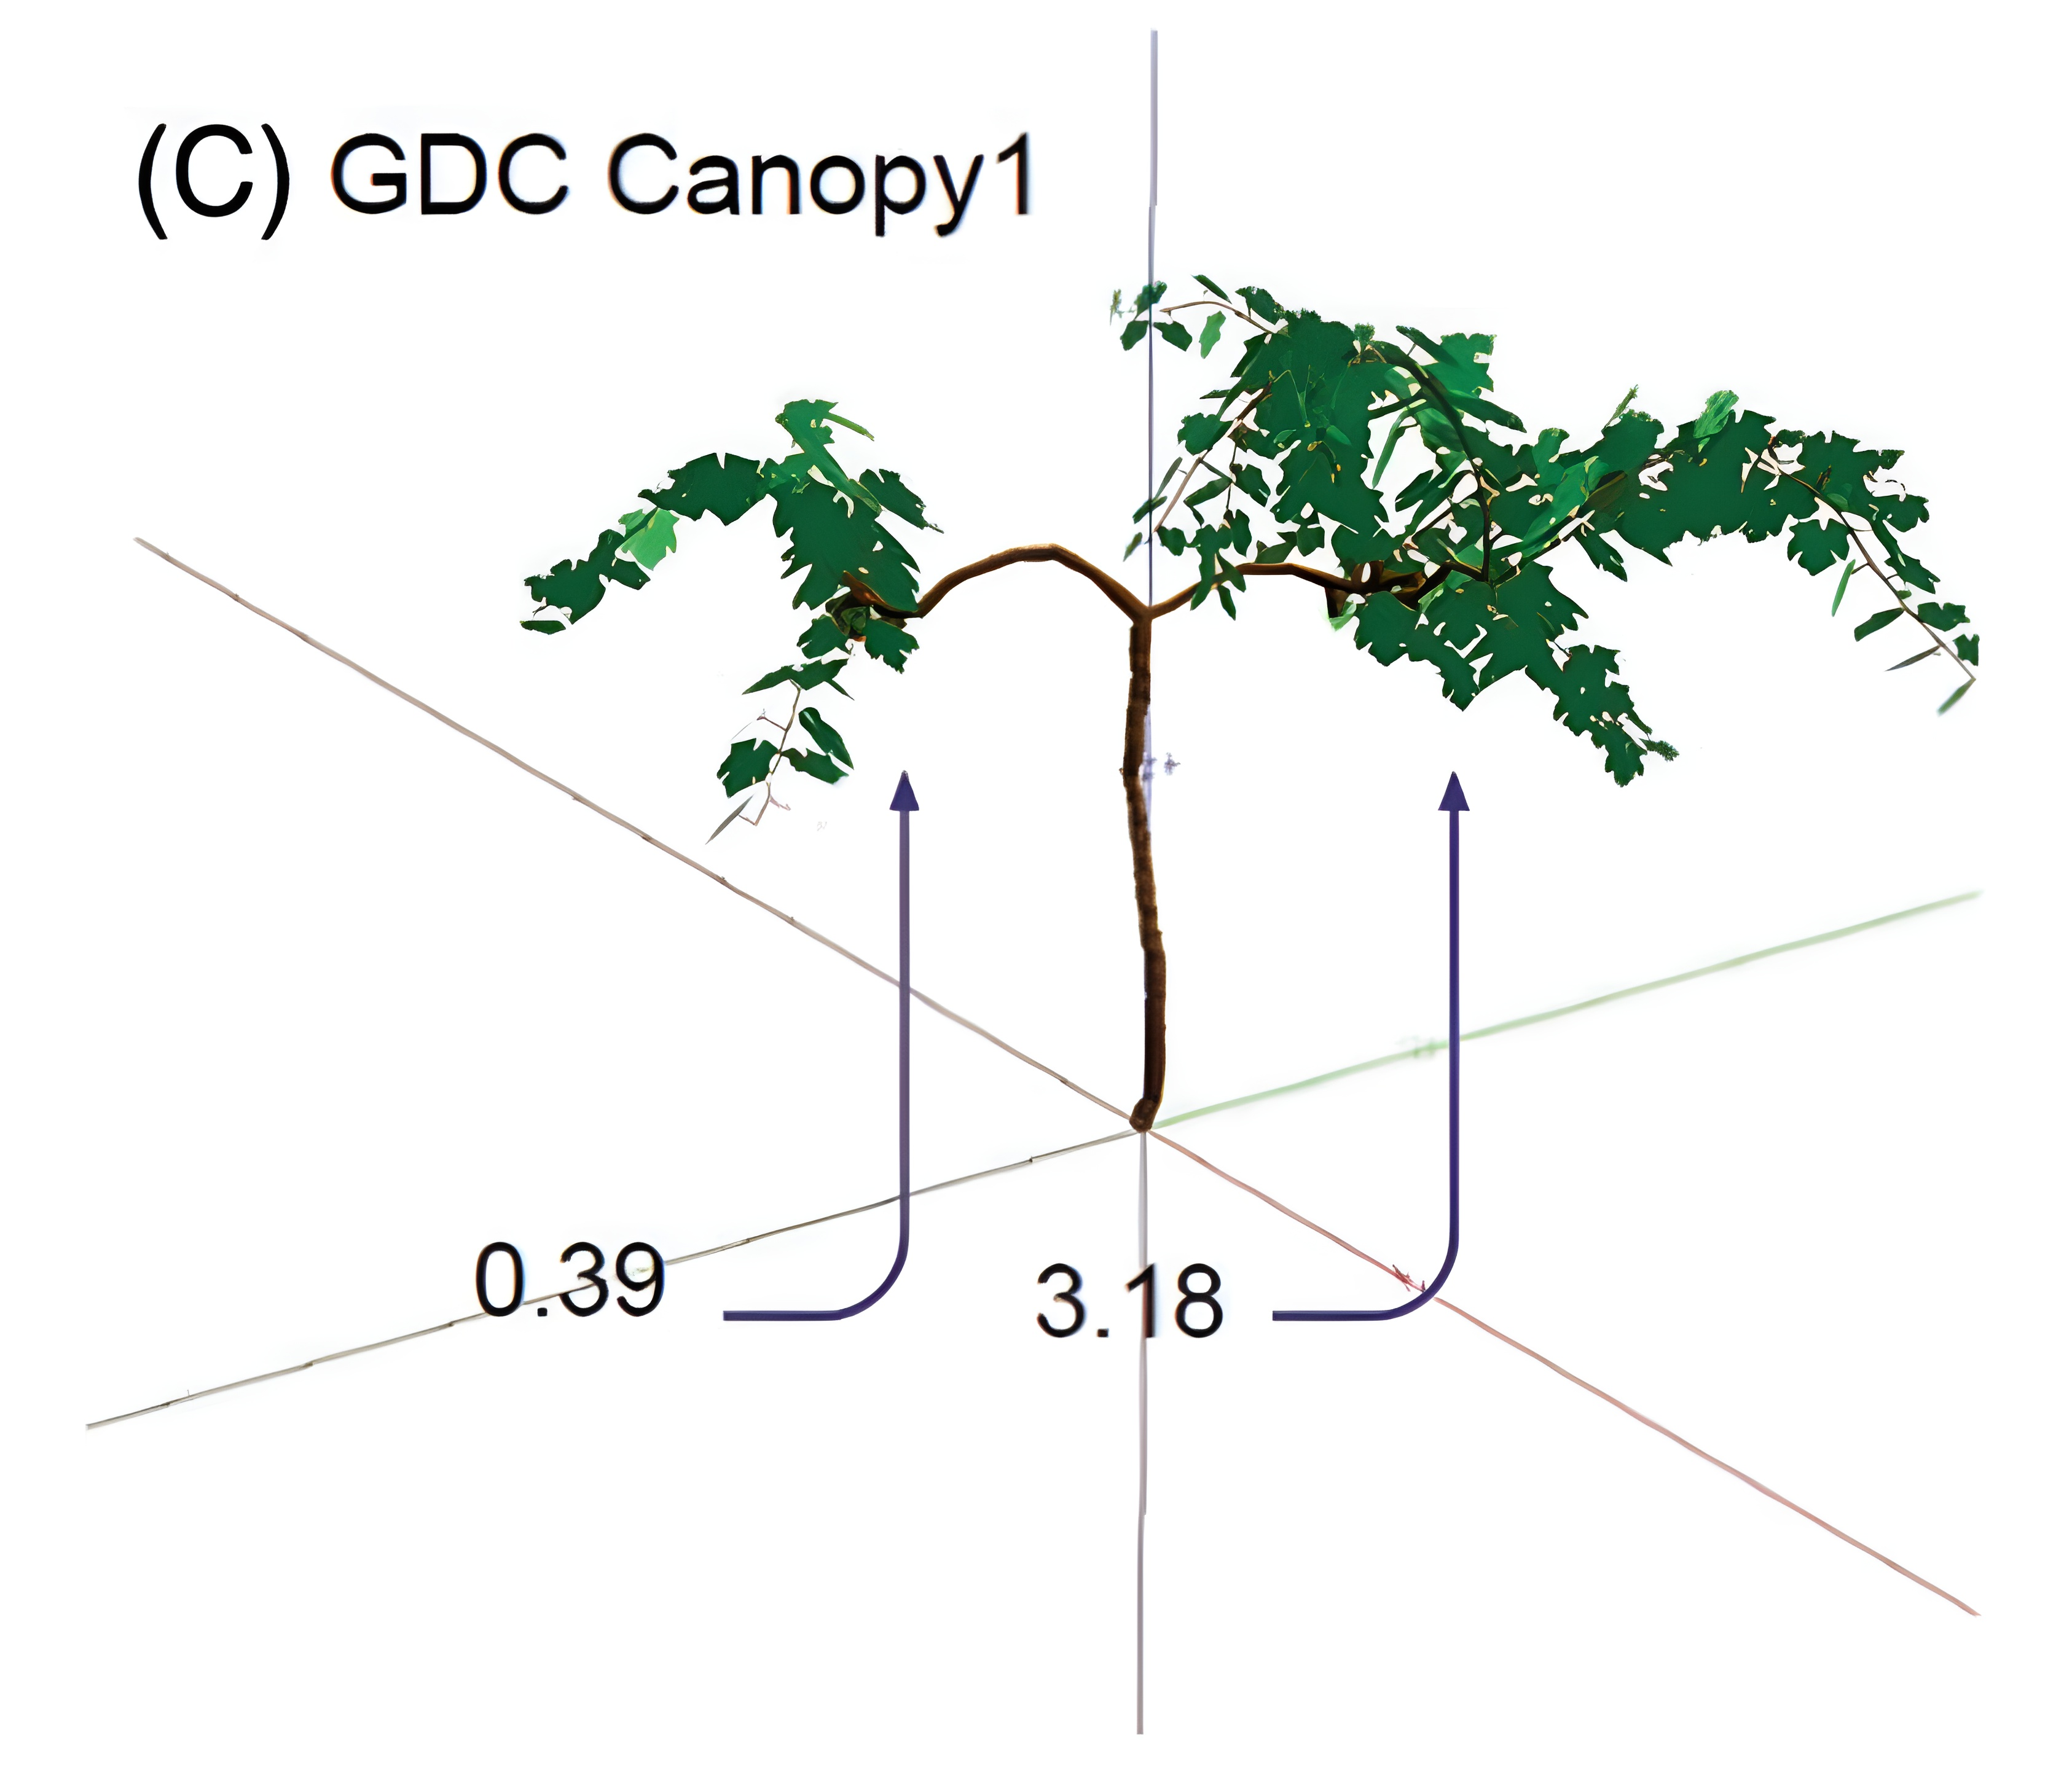
\includegraphics[width=\linewidth,height=\linewidth,keepaspectratio]{img/hydroshoot_can1_upscaled.jpg}
        \caption{HydroShoot}
        \label{fig:hydroshoot-archi}
    \end{subfigure}
    \hfill
    \begin{subfigure}[b]{0.485\linewidth}
        \centering
        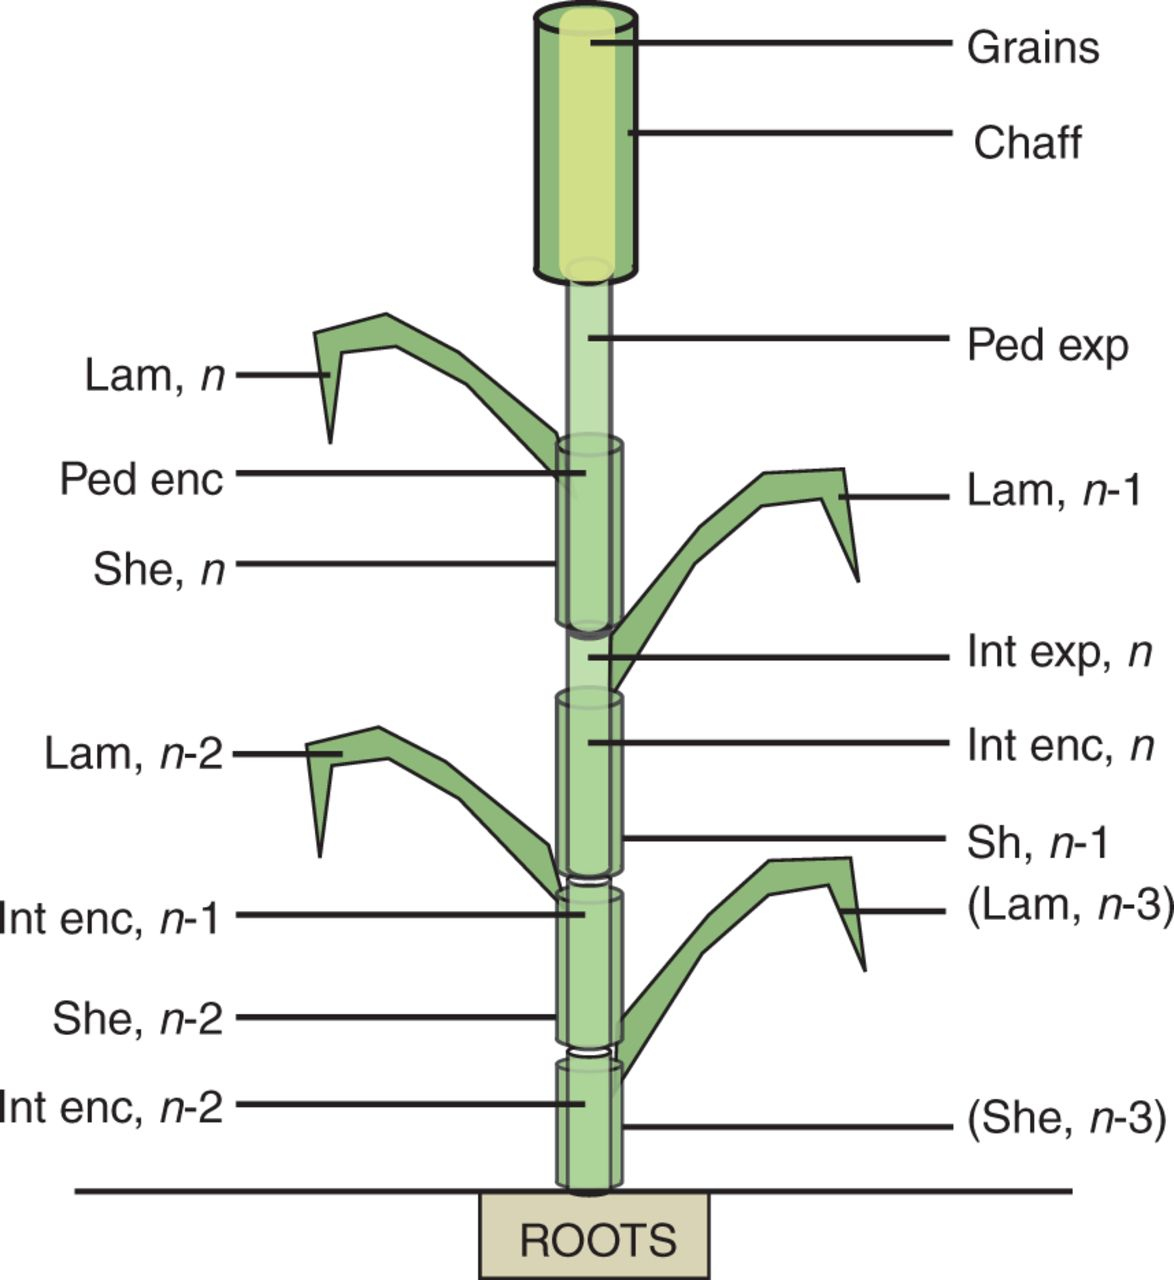
\includegraphics[width=\linewidth,height=0.85\linewidth,keepaspectratio]{img/cnwheat_architecture.jpeg}
        \caption{CN-Wheat}
        \label{fig:cnwheat-archi}
    \end{subfigure}
    \caption[FSPMs selected for use in experiments in this work.]{
            FSPMs selected for use in experiments in this work. 
            (\subref{fig:hydroshoot-archi}) A grapevine specimen from HydroShoot with the canopy trained in the ``Geneva Double Curtain'' configuration.  This figure is reused from \citet{albasha_hydroshoot_2019} under the CC BY 4.0 license.
            (\subref{fig:cnwheat-archi}) The architecture of the CN-Wheat model. This figure is reused from \citet{barillot_cn-wheat_2016} with permission from the publisher (Copyright 2016 Oxford University Press).
    }
    \label{fig:fading_memory_experiments}
\end{figure}

% CC BY 4.0 license

\subsection{Simulation Details}

Table \ref{table:simulation_details} compares the simulation details of both \acrshort{fspm}s.
HydroShoot's simulation length is relatively short, so the simulation must be run multiple times using different meteorological inputs to generate a large enough dataset.
Because of HydroShoot's large size, we will limit our observations to a small selection of leaf elements.
While CN-Wheat only has fifteen elements, we must use an even smaller subset as the reservoir because some physiological targets are a linear function of the elements. 



\begin{table}[!ht]
    \raggedright
    \caption{Comparison of HydroShoot and CN-Wheat: simulation details.}
    \label{table:simulation_details}
    \def\arraystretch{1.2}
    \begin{tabularx}{\textwidth}{
        >{\raggedright\arraybackslash} X
        >{\centering\arraybackslash} X
        >{\centering\arraybackslash} X
    }
        \toprule
        \textbf{} & \textbf{HydroShoot} & \textbf{CN-Wheat} \\ 
        \midrule
        \textbf{Simulation step} & \SI{1}{h} & \SI{1}{h} \\
        \arrayrulecolor{black!10!white}
        \midrule
        \textbf{Simulation duration} & 7 days & 50 days \\
        \midrule
        \textbf{Model structure} & static (idealized reservoir) & Post-vegetative growth \\
        \midrule
        \textbf{Model size} &  $\approx 10^3$ elements & 15 elements \\
        \arrayrulecolor{black}
        \bottomrule
    \end{tabularx}
\end{table}







\subsection{Environmental Inputs}

The environmental inputs of both models are listed in Table \ref{table:simulation_inputs}.
Significant abiotic factors are present in both models: air temperature, relative air humidity, wind speed and incident sunlight.
CO$_2$ concentration and atmospheric pressure are model inputs but use constant values during simulation. 
The available wind speed data for CN-Wheat varies daily instead of hourly, making it unsuited as a regression target or input to computational benchmarks.

% \begin{table}[!ht]
    \raggedright
    \caption{Comparison of HydroShoot and CN-Wheat: environmental models.}
    \label{table:simulation_inputs}
    \def\arraystretch{1.2}
    \begin{tabularx}{\textwidth}{
        >{\centering\arraybackslash} c
        >{\raggedright\arraybackslash} X
        >{\centering\arraybackslash} c
        >{\centering\arraybackslash} c
        >{\centering\arraybackslash} c
    }
        \toprule
        \textbf{Symbol} & \textbf{Description} & \textbf{Unit} & \textbf{HydroShoot} & \textbf{CN-Wheat} \\ 
        \midrule
        \(T_{\text{air}}\) & Air temperature & \unit{\celsius} & Hourly & Hourly \\
        \arrayrulecolor{black!10!white}
        \midrule
        \(\text{RH}\) & Relative humidity & \unit{\percent} & Hourly & Hourly \\
        \midrule
        \(u\) & Wind speed & \unit{\meter\per\second} & Hourly & Daily \\
        \midrule
        \multirow{2}{*}{\(\text{PAR}\)} & \multirow{2}{*}{\acrlong{par}} & \unit{\watt\per\meter\squared} & Hourly & / \\
        % \midrule
        & & \unit{\micro\mole\of{photons}\per\square\metre\per\second} & / & Hourly  \\
        \midrule
        CO\textsubscript{2} & CO\textsubscript{2} concentration & \unit{\micro\mole\of{CO\textsubscript{2}}\per\mol} & \SI{400}{ppm} & \SI{360}{ppm} \\
        \midrule
        \(P_a\) & Atmospheric pressure & \unit{\kilo\pascal} & \SI{101.3}{\kilo\pascal} & / \\
        \arrayrulecolor{black}
        \bottomrule
    \end{tabularx}
\end{table}

% \multirow{6}{6cm}{thermal camera}

% \begin{table}[!ht]
%     \raggedright
%     \caption{Comparison of HydroShoot and CN-Wheat: environmental models.}
%     \label{table:simulation_inputs}
%     \def\arraystretch{1.2}
%     \begin{tabularx}{\textwidth}{
%         >{\centering\arraybackslash} c
%         >{\raggedright\arraybackslash} X
%         >{\centering\arraybackslash} c
%         >{\centering\arraybackslash} c
%         >{\centering\arraybackslash} c
%     }
%         \toprule
%         \textbf{Symbol} & \textbf{Description} & \textbf{Unit} & \textbf{HydroShoot} & \textbf{CN-Wheat} \\ 
%         \midrule
%         \(T_{\text{air}}\) & Air temperature & \unit{\celsius} & Hourly & Hourly \\
%         \arrayrulecolor{black!10!white}
%         \midrule
%         \(\text{RH}\) & Relative humidity & \unit{\percent} & Hourly & Hourly \\
%         \midrule
%         \(u\) & Wind speed & \unit{\meter\per\second} & Hourly & Daily \\
%         \midrule
%         \(R_g\) & Shortwave irradiance & \unit{\watt\per\meter\squared} & Hourly & / \\
%         \midrule
%         \(I_{\text{PAR}}\) & \acrlong{par} & \unit{\micro\mole\of{photons}\per\square\metre\per\second} & / & Hourly  \\
%         \midrule
%         CO\textsubscript{2} & CO\textsubscript{2} concentration & \unit{\micro\mole\of{CO\textsubscript{2}}\per\mol} & \SI{400}{ppm} & \SI{360}{ppm} \\
%         \midrule
%         \(P_a\) & Atmospheric pressure & \unit{\kilo\pascal} & \SI{101.3}{\kilo\pascal} & / \\
%         \arrayrulecolor{black}
%         \bottomrule
%     \end{tabularx}
% \end{table}

\subsection{Regression Targets}

Table \ref{table:simulation_regression_tasks} lists the physiological regression targets that can be used for each model. 
To create more overlap between the two models, it is possible to calculate some targets not present in CN-Wheat from the observed structural elements.

% 
\begin{table}[!ht]
    \raggedright
    \caption[Comparison of HydroShoot and CN-Wheat: available regression tasks.]{Comparison of HydroShoot and CN-Wheat: available regression tasks. Check marks indicate whether the target is computed by the FSPM. Targets annotated with $\ast$ are not calculated in the simulation, but can be computed from other simulation outputs.}
    \label{table:simulation_regression_tasks}
    \def\arraystretch{1.2}
    \begin{tabularx}{\textwidth}{
        >{\centering\arraybackslash} c
        >{\raggedright\arraybackslash} X
        >{\centering\arraybackslash} c
        >{\centering\arraybackslash} c
        >{\centering\arraybackslash} c
    }
        \toprule
        \textbf{Symbol} & \textbf{Description} & \textbf{Unit} & \textbf{HydroShoot} & \textbf{CN-Wheat} \\ 
        \midrule
        \arrayrulecolor{black!10!white}
        \(E\) & Transpiration rate rate & \unit{\gram\per\hour} & \checkmark & \checkmark \\
        \midrule
        \(A_n\) & Net photosynthesis rate & \unit{\micro\mol\per\s} & \checkmark &  \\
        \midrule
        \(T_{\text{leaf}}\) & Mean leaf temperature & \unit{\celsius} & \checkmark & $\ast$ \\
        \midrule
        \multirow{2}{*}{\(\Phi_{\text{PAR}}\)} & \multirow{2}{*}{Absorbed \acrshort{par}} & \unit{\watt\per\meter\squared} & \checkmark &  \\
        % \midrule
        & & \unit{\micro\mol\per\s} & & $\ast$ \\
        \midrule
        \(R_{\text{shoot}}\) & Shoot respiration & \unit{\micro\mol\of{C}\per\second} & & \checkmark  \\
        \midrule
        \(R_{\text{roots}}\) & Root respiration & \unit{\micro\mol\of{C}\per\second} &  & \checkmark  \\
        \arrayrulecolor{black}
        \bottomrule
    \end{tabularx}
\end{table}

% \multirow{6}{6cm}{thermal camera}


% \begin{table}[!ht]
%     \raggedright
%     \caption{Comparison of HydroShoot and CN-Wheat: available regression tasks. Targets annotated with $\ast$ are not calculated in the simulation, but can be computed from other simulation outputs.}
%     \label{table:simulation_regression_tasks}
%     \def\arraystretch{1.2}
%     \begin{tabularx}{\textwidth}{
%         >{\centering\arraybackslash} c
%         >{\raggedright\arraybackslash} X
%         >{\centering\arraybackslash} c
%         >{\centering\arraybackslash} c
%         >{\centering\arraybackslash} c
%     }
%         \toprule
%         \textbf{Symbol} & \textbf{Description} & \textbf{Unit} & \textbf{HydroShoot} & \textbf{CN-Wheat} \\ 
%         \midrule
%         \arrayrulecolor{black!10!white}
%         \(E\) & Transpiration rate rate & \unit{\gram\per\hour} & \checkmark & \checkmark \\
%         \midrule
%         \(A_n\) & Net photosynthesis rate & \unit{\micro\mol\per\s} & \checkmark &  \\
%         \midrule
%         \(T_{\text{leaf}}\) & Mean leaf temperature & \unit{\celsius} & \checkmark & $\ast$ \\
%         \midrule
%         \(\Phi_{R_g}\) & Absorbed solar irradiance & \unit{\watt\per\meter\squared} & \checkmark &  \\
%         \midrule
%         \(\Phi_{I_\text{PAR}}\) & Absorbed \acrshort{par} & \unit{\micro\mol\per\s} & & $\ast$ \\
%         \midrule
%         \(R_{\text{shoot}}\) & Shoot respiration & \unit{??} & & \checkmark  \\
%         \midrule
%         \(R_{\text{roots}}\) & Root respiration & \unit{??} &  & \checkmark  \\
%         \arrayrulecolor{black}
%         \bottomrule
%     \end{tabularx}
% \end{table}

\subsection{Available Reservoirs}

The observable physiological processes for HydroShoot and CN-Wheat are presented in Table \ref{table:simulation_reservoirs}.
We limited the table to processes that would be experimentally observable, as listed in Tables \ref{table:imaging-techniques} and \ref{table:non-imaging-techniques}. 
Both models track the photosynthesis rate, surface temperature, transpiration rate, and stomatal conductance. 
HydroShoot has some additional hydraulic processes available.

% 
\begin{table}[!ht]
    \raggedright
    \caption[Comparison of HydroShoot and CN-Wheat: physiological processes observable in each structural element.]{Comparison of HydroShoot and CN-Wheat: physiological processes observable in each structural element. Not all are shown in the table; we only present the processes that are experimentally observable and that do not violate \acrshort{rc} assumptions in an obvious way. Check marks indicate whether the physiological process is modeled by the FSPM.}
    \label{table:simulation_reservoirs}
    \def\arraystretch{1.2}
    \begin{tabularx}{\textwidth}{
        >{\centering\arraybackslash} c
        >{\raggedright\arraybackslash} X
        >{\centering\arraybackslash} c
        >{\centering\arraybackslash} c
        >{\centering\arraybackslash} c
    }
        \toprule
        \textbf{Symbol} & \textbf{Description} & \textbf{Unit} & \textbf{HydroShoot} & \textbf{CN-Wheat} \\ 
        \midrule
        \(A_n\) & Net photosynthesis rate & \unit{\micro\mol\per\meter\squared\per\second} & \checkmark & \checkmark \\
        \arrayrulecolor{black!10!white}
        \midrule
        \(T_s\) & Surface temperature & \unit{\celsius} & \checkmark & \checkmark \\
        \midrule
        \(g_s\) & Stomatal conductance & \unit{\mol\per\meter\squared\per\second} & \checkmark & \checkmark \\
        \midrule
        \(E\) & Transpiration rate & \unit{\mol\of{H\textsubscript{2}O}\per\meter\squared\per\second} & \checkmark & \checkmark \\
        \midrule
        \(F\) & Water flow across segment & \unit{\kilo\gram\per\second} & \checkmark &  \\
        \midrule
        \(\Psi\) & Mean water potential of segment & \unit{\mega\pascal} & \checkmark &  \\
        \arrayrulecolor{black}
        \bottomrule
    \end{tabularx}
\end{table}

      
      

\section{Summary}

First, we formalized the selection criteria to choose which plant models are suited for our research.
We based these criteria on considerations from an \acrshort{rc}, a plant-physiological, and a practical perspective.
Next, we held a brief discussion of each \acrshort{fspm} we considered from the literature.
Then, we made a final selection of two models: HydroShoot and CN-Wheat.
We introduced the background of each model and gave its implementation details.
Finally, we summarized their properties relevant to our experiments: the environmental inputs, the available regression targets, and the observations that can be used as a reservoir.


\begin{table}[!ht]
    \raggedright
    \caption{Comparison of HydroShoot and CN-Wheat: environmental models.}
    \label{table:simulation_inputs}
    \def\arraystretch{1.2}
    \begin{tabularx}{\textwidth}{
        >{\centering\arraybackslash} c
        >{\raggedright\arraybackslash} X
        >{\centering\arraybackslash} c
        >{\centering\arraybackslash} c
        >{\centering\arraybackslash} c
    }
        \toprule
        \textbf{Symbol} & \textbf{Description} & \textbf{Unit} & \textbf{HydroShoot} & \textbf{CN-Wheat} \\ 
        \midrule
        \(T_{\text{air}}\) & Air temperature & \unit{\celsius} & Hourly & Hourly \\
        \arrayrulecolor{black!10!white}
        \midrule
        \(\text{RH}\) & Relative humidity & \unit{\percent} & Hourly & Hourly \\
        \midrule
        \(u\) & Wind speed & \unit{\meter\per\second} & Hourly & Daily \\
        \midrule
        \multirow{2}{*}{\(\text{PAR}\)} & \multirow{2}{*}{\acrlong{par}} & \unit{\watt\per\meter\squared} & Hourly & / \\
        % \midrule
        & & \unit{\micro\mole\of{photons}\per\square\metre\per\second} & / & Hourly  \\
        \midrule
        CO\textsubscript{2} & CO\textsubscript{2} concentration & \unit{\micro\mole\of{CO\textsubscript{2}}\per\mol} & \SI{400}{ppm} & \SI{360}{ppm} \\
        \midrule
        \(P_a\) & Atmospheric pressure & \unit{\kilo\pascal} & \SI{101.3}{\kilo\pascal} & / \\
        \arrayrulecolor{black}
        \bottomrule
    \end{tabularx}
\end{table}

% \multirow{6}{6cm}{thermal camera}

% \begin{table}[!ht]
%     \raggedright
%     \caption{Comparison of HydroShoot and CN-Wheat: environmental models.}
%     \label{table:simulation_inputs}
%     \def\arraystretch{1.2}
%     \begin{tabularx}{\textwidth}{
%         >{\centering\arraybackslash} c
%         >{\raggedright\arraybackslash} X
%         >{\centering\arraybackslash} c
%         >{\centering\arraybackslash} c
%         >{\centering\arraybackslash} c
%     }
%         \toprule
%         \textbf{Symbol} & \textbf{Description} & \textbf{Unit} & \textbf{HydroShoot} & \textbf{CN-Wheat} \\ 
%         \midrule
%         \(T_{\text{air}}\) & Air temperature & \unit{\celsius} & Hourly & Hourly \\
%         \arrayrulecolor{black!10!white}
%         \midrule
%         \(\text{RH}\) & Relative humidity & \unit{\percent} & Hourly & Hourly \\
%         \midrule
%         \(u\) & Wind speed & \unit{\meter\per\second} & Hourly & Daily \\
%         \midrule
%         \(R_g\) & Shortwave irradiance & \unit{\watt\per\meter\squared} & Hourly & / \\
%         \midrule
%         \(I_{\text{PAR}}\) & \acrlong{par} & \unit{\micro\mole\of{photons}\per\square\metre\per\second} & / & Hourly  \\
%         \midrule
%         CO\textsubscript{2} & CO\textsubscript{2} concentration & \unit{\micro\mole\of{CO\textsubscript{2}}\per\mol} & \SI{400}{ppm} & \SI{360}{ppm} \\
%         \midrule
%         \(P_a\) & Atmospheric pressure & \unit{\kilo\pascal} & \SI{101.3}{\kilo\pascal} & / \\
%         \arrayrulecolor{black}
%         \bottomrule
%     \end{tabularx}
% \end{table}

\begin{table}[!ht]
    \raggedright
    \caption[Comparison of HydroShoot and CN-Wheat: available regression tasks.]{Comparison of HydroShoot and CN-Wheat: available regression tasks. Check marks indicate whether the target is computed by the FSPM. Targets annotated with $\ast$ are not calculated in the simulation, but can be computed from other simulation outputs.}
    \label{table:simulation_regression_tasks}
    \def\arraystretch{1.2}
    \begin{tabularx}{\textwidth}{
        >{\centering\arraybackslash} c
        >{\raggedright\arraybackslash} X
        >{\centering\arraybackslash} c
        >{\centering\arraybackslash} c
        >{\centering\arraybackslash} c
    }
        \toprule
        \textbf{Symbol} & \textbf{Description} & \textbf{Unit} & \textbf{HydroShoot} & \textbf{CN-Wheat} \\ 
        \midrule
        \arrayrulecolor{black!10!white}
        \(E\) & Transpiration rate rate & \unit{\gram\per\hour} & \checkmark & \checkmark \\
        \midrule
        \(A_n\) & Net photosynthesis rate & \unit{\micro\mol\per\s} & \checkmark &  \\
        \midrule
        \(T_{\text{leaf}}\) & Mean leaf temperature & \unit{\celsius} & \checkmark & $\ast$ \\
        \midrule
        \multirow{2}{*}{\(\Phi_{\text{PAR}}\)} & \multirow{2}{*}{Absorbed \acrshort{par}} & \unit{\watt\per\meter\squared} & \checkmark &  \\
        % \midrule
        & & \unit{\micro\mol\per\s} & & $\ast$ \\
        \midrule
        \(R_{\text{shoot}}\) & Shoot respiration & \unit{\micro\mol\of{C}\per\second} & & \checkmark  \\
        \midrule
        \(R_{\text{roots}}\) & Root respiration & \unit{\micro\mol\of{C}\per\second} &  & \checkmark  \\
        \arrayrulecolor{black}
        \bottomrule
    \end{tabularx}
\end{table}

% \multirow{6}{6cm}{thermal camera}


% \begin{table}[!ht]
%     \raggedright
%     \caption{Comparison of HydroShoot and CN-Wheat: available regression tasks. Targets annotated with $\ast$ are not calculated in the simulation, but can be computed from other simulation outputs.}
%     \label{table:simulation_regression_tasks}
%     \def\arraystretch{1.2}
%     \begin{tabularx}{\textwidth}{
%         >{\centering\arraybackslash} c
%         >{\raggedright\arraybackslash} X
%         >{\centering\arraybackslash} c
%         >{\centering\arraybackslash} c
%         >{\centering\arraybackslash} c
%     }
%         \toprule
%         \textbf{Symbol} & \textbf{Description} & \textbf{Unit} & \textbf{HydroShoot} & \textbf{CN-Wheat} \\ 
%         \midrule
%         \arrayrulecolor{black!10!white}
%         \(E\) & Transpiration rate rate & \unit{\gram\per\hour} & \checkmark & \checkmark \\
%         \midrule
%         \(A_n\) & Net photosynthesis rate & \unit{\micro\mol\per\s} & \checkmark &  \\
%         \midrule
%         \(T_{\text{leaf}}\) & Mean leaf temperature & \unit{\celsius} & \checkmark & $\ast$ \\
%         \midrule
%         \(\Phi_{R_g}\) & Absorbed solar irradiance & \unit{\watt\per\meter\squared} & \checkmark &  \\
%         \midrule
%         \(\Phi_{I_\text{PAR}}\) & Absorbed \acrshort{par} & \unit{\micro\mol\per\s} & & $\ast$ \\
%         \midrule
%         \(R_{\text{shoot}}\) & Shoot respiration & \unit{??} & & \checkmark  \\
%         \midrule
%         \(R_{\text{roots}}\) & Root respiration & \unit{??} &  & \checkmark  \\
%         \arrayrulecolor{black}
%         \bottomrule
%     \end{tabularx}
% \end{table}

\begin{table}[!ht]
    \raggedright
    \caption[Comparison of HydroShoot and CN-Wheat: physiological processes observable in each structural element.]{Comparison of HydroShoot and CN-Wheat: physiological processes observable in each structural element. Not all are shown in the table; we only present the processes that are experimentally observable and that do not violate \acrshort{rc} assumptions in an obvious way. Check marks indicate whether the physiological process is modeled by the FSPM.}
    \label{table:simulation_reservoirs}
    \def\arraystretch{1.2}
    \begin{tabularx}{\textwidth}{
        >{\centering\arraybackslash} c
        >{\raggedright\arraybackslash} X
        >{\centering\arraybackslash} c
        >{\centering\arraybackslash} c
        >{\centering\arraybackslash} c
    }
        \toprule
        \textbf{Symbol} & \textbf{Description} & \textbf{Unit} & \textbf{HydroShoot} & \textbf{CN-Wheat} \\ 
        \midrule
        \(A_n\) & Net photosynthesis rate & \unit{\micro\mol\per\meter\squared\per\second} & \checkmark & \checkmark \\
        \arrayrulecolor{black!10!white}
        \midrule
        \(T_s\) & Surface temperature & \unit{\celsius} & \checkmark & \checkmark \\
        \midrule
        \(g_s\) & Stomatal conductance & \unit{\mol\per\meter\squared\per\second} & \checkmark & \checkmark \\
        \midrule
        \(E\) & Transpiration rate & \unit{\mol\of{H\textsubscript{2}O}\per\meter\squared\per\second} & \checkmark & \checkmark \\
        \midrule
        \(F\) & Water flow across segment & \unit{\kilo\gram\per\second} & \checkmark &  \\
        \midrule
        \(\Psi\) & Mean water potential of segment & \unit{\mega\pascal} & \checkmark &  \\
        \arrayrulecolor{black}
        \bottomrule
    \end{tabularx}
\end{table}

      
      

\chapter{Implementation Details} \label{chapter:methods}

% Introduction
Chapter \ref{chapter:exp-setup} established the experimental framework for this work.
Then, Chapter \ref{chapter:models-used} detailed the two \acrshort{fspm}s we selected for our experiments.
In this chapter, we explain how we implemented the experiments.
We discuss the adaptations that we made to the simulations, how we handled data for the regression tasks, and how we implemented the impulse experiment.


\section{Preparing the Simulations}

We used the same environmental inputs as the models' original publications for all experiments because the authors only verified the models for these climate conditions.
The complete hourly data for HydroShoot and CN-Wheat can be found in \mbox{Appendix \ref{app:meteo}}.
HydroShoot required small adaptations to the soil water model because empirical soil water data was only available for four consecutive dates. 
We ran CN-Wheat simulations with no modifications.
Details for reproducing the exact simulation setup for both models, as well as descriptions of model modifications we made can be found in Appendices \ref{app:hydroshoot-sim-details} and \ref{app:cnwheat-simulation}.


\section{Observing The Plant Model}

We extracted time series for all physiological processes listed in \mbox{Table \ref{table:simulation_reservoirs}} from each structural element of the \acrshort{fspm}.
The reservoirs are then constructed from this data.
This work investigates homogeneous reservoirs only; we only considered the spatial variations of a single process, not the dynamics between two or more processes. 
However, some preliminary work with heterogeneous reservoirs showed promising results, which can be explored in further research.

It is impossible to get exact measurements or observe the entire plant at once in a real-world scenario.
To make our results more representative for follow-up research, we decided only to observe a fraction of the plant's structure to limit the observability of the reservoir.
We used a reservoir sample size of 32 for HydroShoot and 7 for CN-Wheat. 
This corresponds with approximately \SI{10}{\percent} and \SI{70}{\percent} of the total structure, respectively.
We chose 32 for HydroShoot to limit the number of readout parameters and because we observed that the reservoir performance showed negligible improvements for larger sample sizes.
We only had ten structural elements to observe the chosen physiological processes in CN-Wheat. 
We selected a sample size of 7 to avoid the total observability of the reservoir.
Observing the entire reservoir may introduce bias as the plant model uses the same observations to compute the physiological tasks.
Appendices \ref{app:hydroshoot-reservoir} and \ref{app:cnwheat-reservoir} further elaborate on how the reservoir was constructed for HydroShoot and CN-Wheat, respectively.

% TODO (OPTIONAL): Add figma illustration showing a sketch of a plant, then zoom in on one structural element, then zoom in on the series extracted from it.

\section{Data Preprocessing} \label{sec:data-preprocessing}

First, the raw simulation outputs are combined into a single dataset. Appendices \ref{app:hydroshoot-dataset} and \ref{app:cnwheat-dataset} explain how we did this for each model specifically.
Once we have a single dataset, some preprocessing steps are applied.
Next, we discarded data from the first four days of each simulation run to avoid transient dynamics present during model warm-up.
We also discarded 8 hours of nighttime from each day, between 22:00 and 4:00.
% The considered physiological processes fall idle during these hours.
By discarding these samples from the dataset, we focus the model's capacity on predicting the more detailed and intricate daytime dynamics instead of concentrating on the broader day/night dynamic.
Figure \ref{fig:preprocessing-train-test-split} illustrates the data that is discarded.

Finally, we rescaled both the target and the reservoir series to have zero mean and unit variance.
When we scaled each dimension independently, we noticed a drop in model performance.
We hypothesize that this is due to lost information about the relative difference between observed elements.
Because the observations of the reservoir elements are not independent of each other, we instead rescaled the reservoir using the mean and variance of the reservoir as a whole.

\section{Train and Test Data Split} \label{sec:train-test-split}

To avoid bias in the model scores, we require a set of unseen test data to validate the performance of the final model.
Therefore the optimal model parameters should be trained using only a subset of the total dataset.
We used a train-to-test ratio of 0.5 for all our regression experiments.
Figure \ref{fig:preprocessing-train-test-split} shows how we divided the data samples into train and test sets.
Time series data naturally shows a high degree of temporal correlation.
To reduce the surface area for information leaking between train and test sets, we divided the data into blocks of four days.
The previously mentioned process of discarding the nighttime samples further limits the information leakage between adjacent blocks of train and test data.
% Because the samples from the same day are highly temporally correlated, we grouped the data in blocks of 24 hours that should stay together.
% We then assign the groups to the train or test set in alternating blocks of 4 days.
% This further decreases the information leakage between training and testing data.

\begin{figure}[ht]
	\centering
    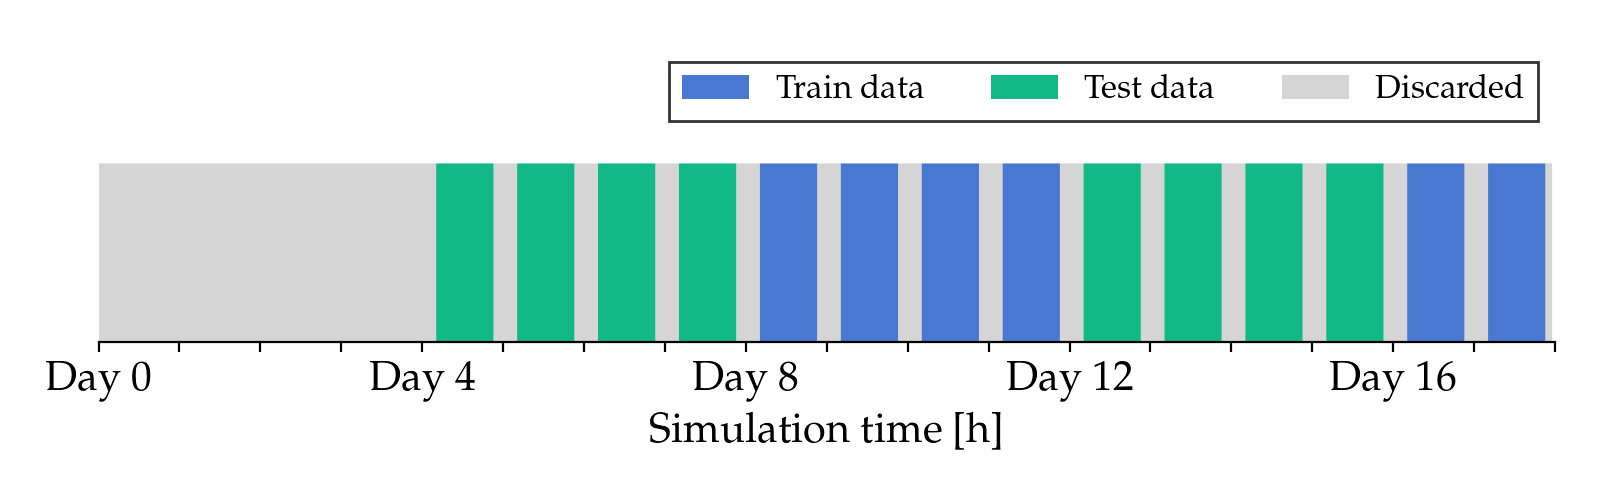
\includegraphics[width=13.33cm]{img/preprocessing_traintestsplit.png}
	\caption[Illustration of the data that is discarded as a preprocessing step and how the remaining data is split into a train and test set.]{Illustration of the data that is discarded as a preprocessing step and how the remaining data is split into a train and test set.}
	\label{fig:preprocessing-train-test-split}
\end{figure}

\section{Model Validation} \label{methods:validation}

The model parameters for each reservoir-target pairing are fitted using ridge regression (\mbox{Equation \ref{esn:training}}).
To find the optimal regularization parameter $\lambda$, we performed a parameter sweep from 0.0001 to 100 with fifty logarithmically spaced values.
We validated the choice of $\lambda$ using the cross-validation method.
In this scheme, the training data is split into ``folds'' of roughly equal size. 
The model is trained using data from all but one fold.
The final fold is used to validate the model, using the \acrshort{nmse} metric.
We repeat this until we have used all folds as validation data.
The mean \acrshort{nmse} across all validation folds suggests the model performance for that value of $\lambda$.
We pick the value of $\lambda$ that yields the best mean validation score.
Once the optimal $\lambda$ is selected, we train a final model using all available training data.

Figure \ref{fig:methods-cv-folds} shows how we created our cross-validation folds. 
We group the folds per calendar day to avoid putting data from the same simulation day in both the train and validation sets.
Otherwise, we risk introducing bias in the validation score thanks to the high temporal correlation between samples of the same input day.
We used the leave-one-group-out strategy, which means we used only one day of data for validation in each iteration.
See Appendices \ref{app:hydroshoot-validation} and \ref{app:cnwheat-validation} for plant information specific to the HydroShoot and CN-Wheat datasets.
% Groups of data samples from the same input day stay together; otherwise, we leak highly correlated data between the train and validation data.

\begin{figure}[ht]
	\centering
    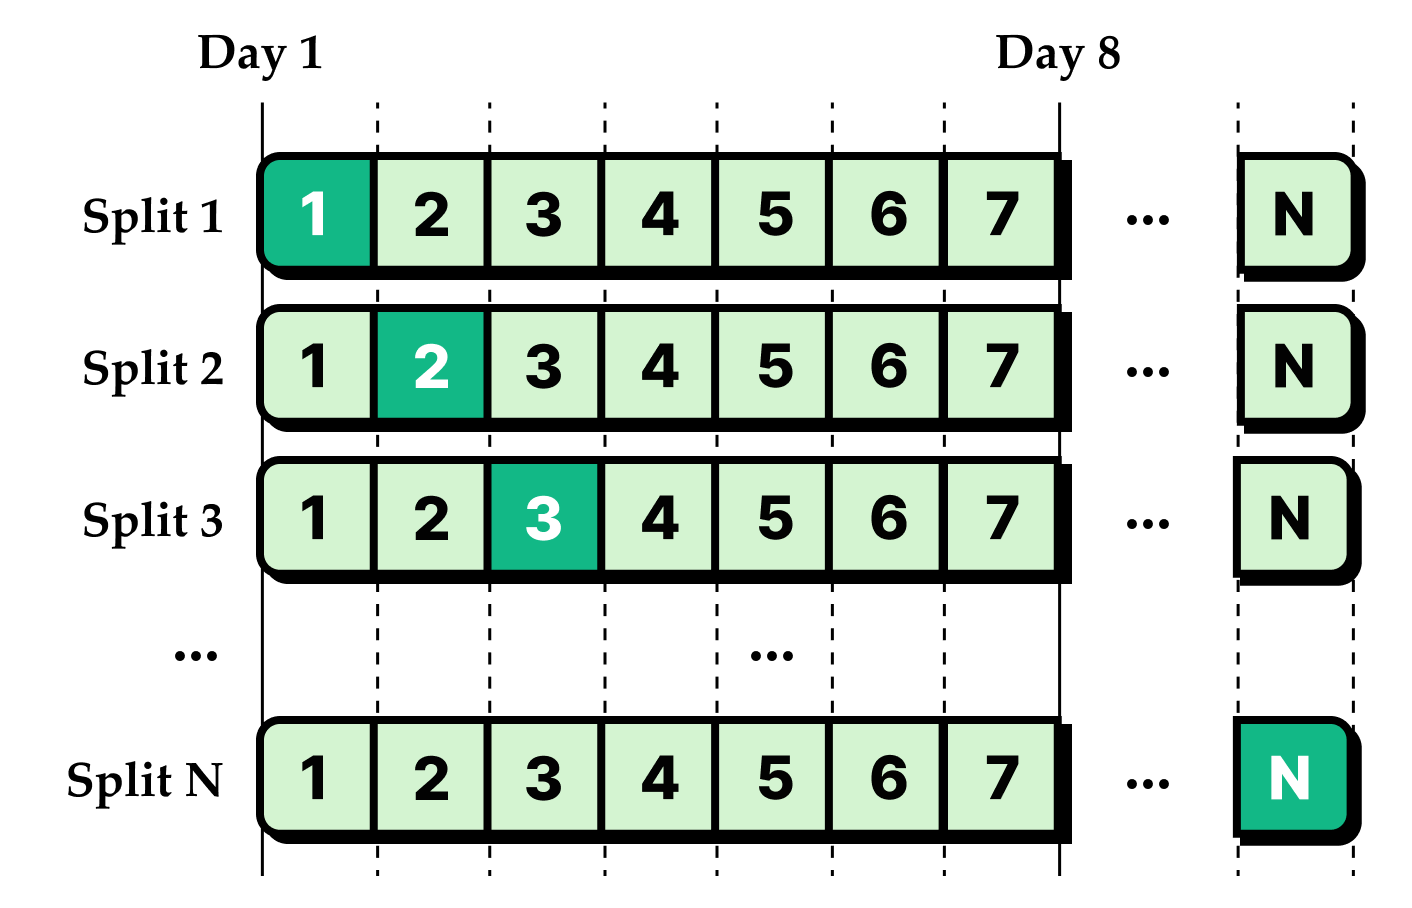
\includegraphics[width=10.5cm]{img/cv-folds.png}
	\caption[Illustration of leave-one-group-out cross-validation strategy.]{Leave-one-group-out cross-validation strategy. Each block represents samples generated from the same calendar day of meteorological inputs. In each split, the highlighted data is used as validation data, the other folds are used for training.}
	\label{fig:methods-cv-folds}
\end{figure}


\section{Implementing the Impulse Experiment}

To implement the impulse experiment, we modified the meteorological input data before running the simulations.
Figure \ref{fig:methods-impulse} demonstrates how the impulse is added to an environmental signal.
The stimulus was applied at least four days after the simulation started to account for transient warmup dynamics in the plant model.
We chose four days because this is the same as the warmup period we assumed in \mbox{Section \ref{sec:data-preprocessing}}.
The model is allowed to run at least five more days after the impulse to capture the fading memory effect completely.
The impulse is always centered on midday and is applied instantaneously.
Appendices \ref{app:hydroshoot-impulse} and \ref{app:cnwheat-impulse} disclose the exact simulation configuration for HydroShoot and CN-Wheat respectively.

\begin{figure}[]
	\centering
    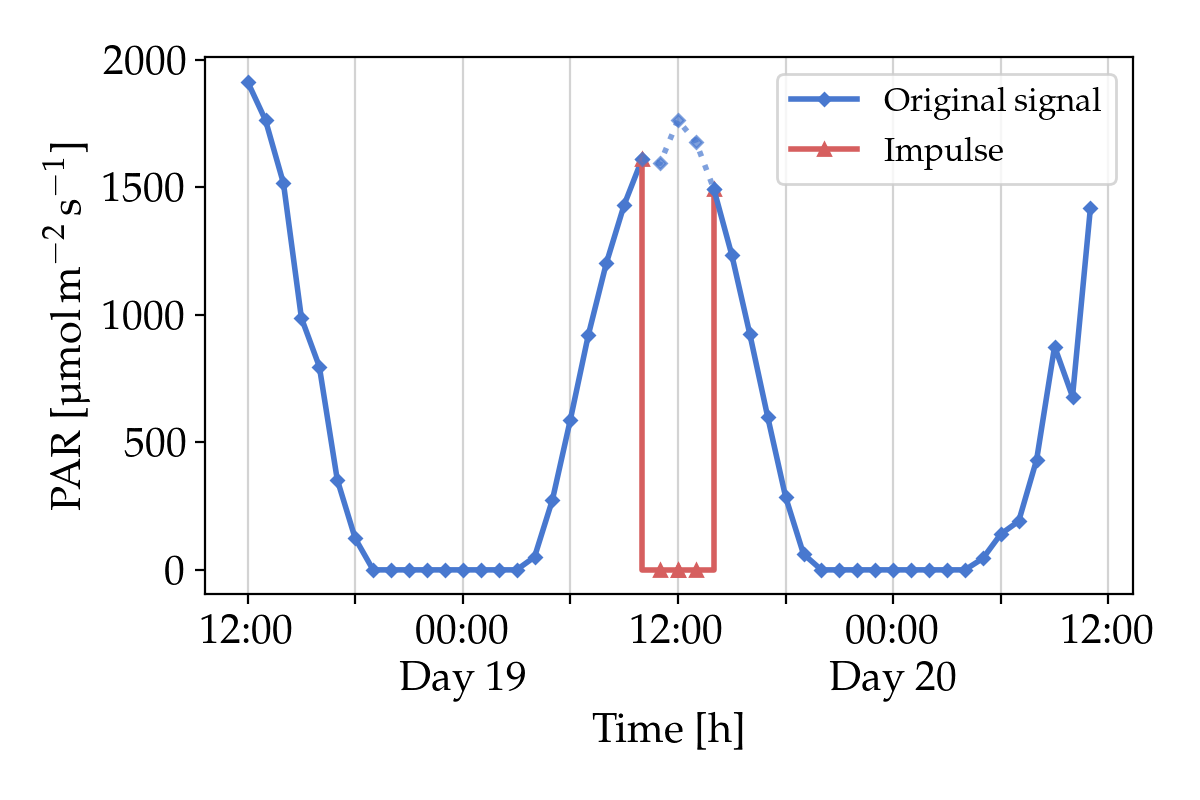
\includegraphics[width=10cm]{img/cn_impulse.png}
	\caption[Adding an artificial impulse to an environmental input.]{Adding an artificial impulse to an environmental input. In this figure we applied an impulse with a width of three hours and a value of \SI{0}{\micro\mole\per\square\meter\per\second} to the incident \acrshort{par} of CN-Wheat.}
	\label{fig:methods-impulse}
\end{figure}

\section{Summary}

This chapter disclosed the implementation details required to reproduce the experimental results presented in this work.
We discussed how the reservoir dataset is constructed, what data preprocessing is applied, how a test dataset is created, and we how validated the readout model parameters. 
We also documented how we implemented the impulse experiment.
We reported additional information on how HydroShoot and CN-Wheat were used in Appendices \ref{app:hydroshoot} and \ref{app:cnwheat}.



\part{Results}
\chapter{Results And Discussion} \label{chapter:results}

% Chapter introduction
In this chapter we apply the framework established in \mbox{Chapter \ref{chapter:exp-setup}} to the \acrshort{fspm}s we selected in Chapter \ref{chapter:models-used}.
With this framework, we tested the reservoir characteristics of each of the physiological processes in Table \ref{table:simulation_reservoirs}.
We first study the linear input separation for physiologically relevant regression tasks.
Then, we examine the fading memory property of the considered physiological processes. 
Finally, we point out some weaknesses in our methods and how they could have been mitigated.


\section{Input Separation} \label{results:input-sep}

% Introduction input separation
We used several regression tasks to test the linear input separation in the physiological reservoirs.
These tasks fall into three categories: (i) predicting current environmental conditions, (ii) predicting the plant's eco-physiological performance, and (iii) computational benchmarks.
For the reservoir readout, we used a random sample of the plant structure, with a size of 32 and 7 for HydroShoot and CN-Wheat, respectively.
We considered 16 different random reservoir samples for each plant model to determine the performance variability caused by the selected observations.


\subsection{Environmental Inputs and Physiological Tasks}

% Input and physiological task regression scores
Let us first consider categories (i) and (ii).
For the environmental targets, we considered air temperature ($T_{\text{air}}$), relative humidity (RH) and incident photosynthetically active radiation (PAR).
We chose these targets because of their physiological relevance and to compare the results with those already obtained for strawberry plants in \citet{pieters_reservoir_2022}.
For the physiological targets we used transpiration rate ($E$), absorbed PAR ($\Phi_{\text{PAR}}$) and net photosynthesis rate ($A_n$). 
$A_n$ was only available in HydroShoot.
% The latter was only available in HydroShoot.

Figure \ref{fig:input-phys-scores} showcases the performance of each physiological reservoir as boxplots.
For the HydroShoot model, we observe that each reservoir performs roughly the same for a given target.
In CN-Wheat, the difference between the reservoirs is more outspoken.
For example, RH correlates relatively well with $E$ in CN-Wheat, where none of the processes in HydroShoot correlate well with RH.
We must also note that CN-Wheat significantly outperforms HydroShoot in most tasks.
% This disparity can partly be attributed to the larger relative observability of the CN-Wheat model; 
% for CN-Wheat, we observed \SI{70}{\percent} of the structural elements compared to only \SI{8.9}{\percent} for HydroShoot.
% The impact of observability is particularly noticeable in $\Phi_{\text{PAR}}$, where CN-Wheat achieves near-perfect accuracy with the $A_n$ and $E$ reservoirs.

\begin{figure}[hp]
	\centering
    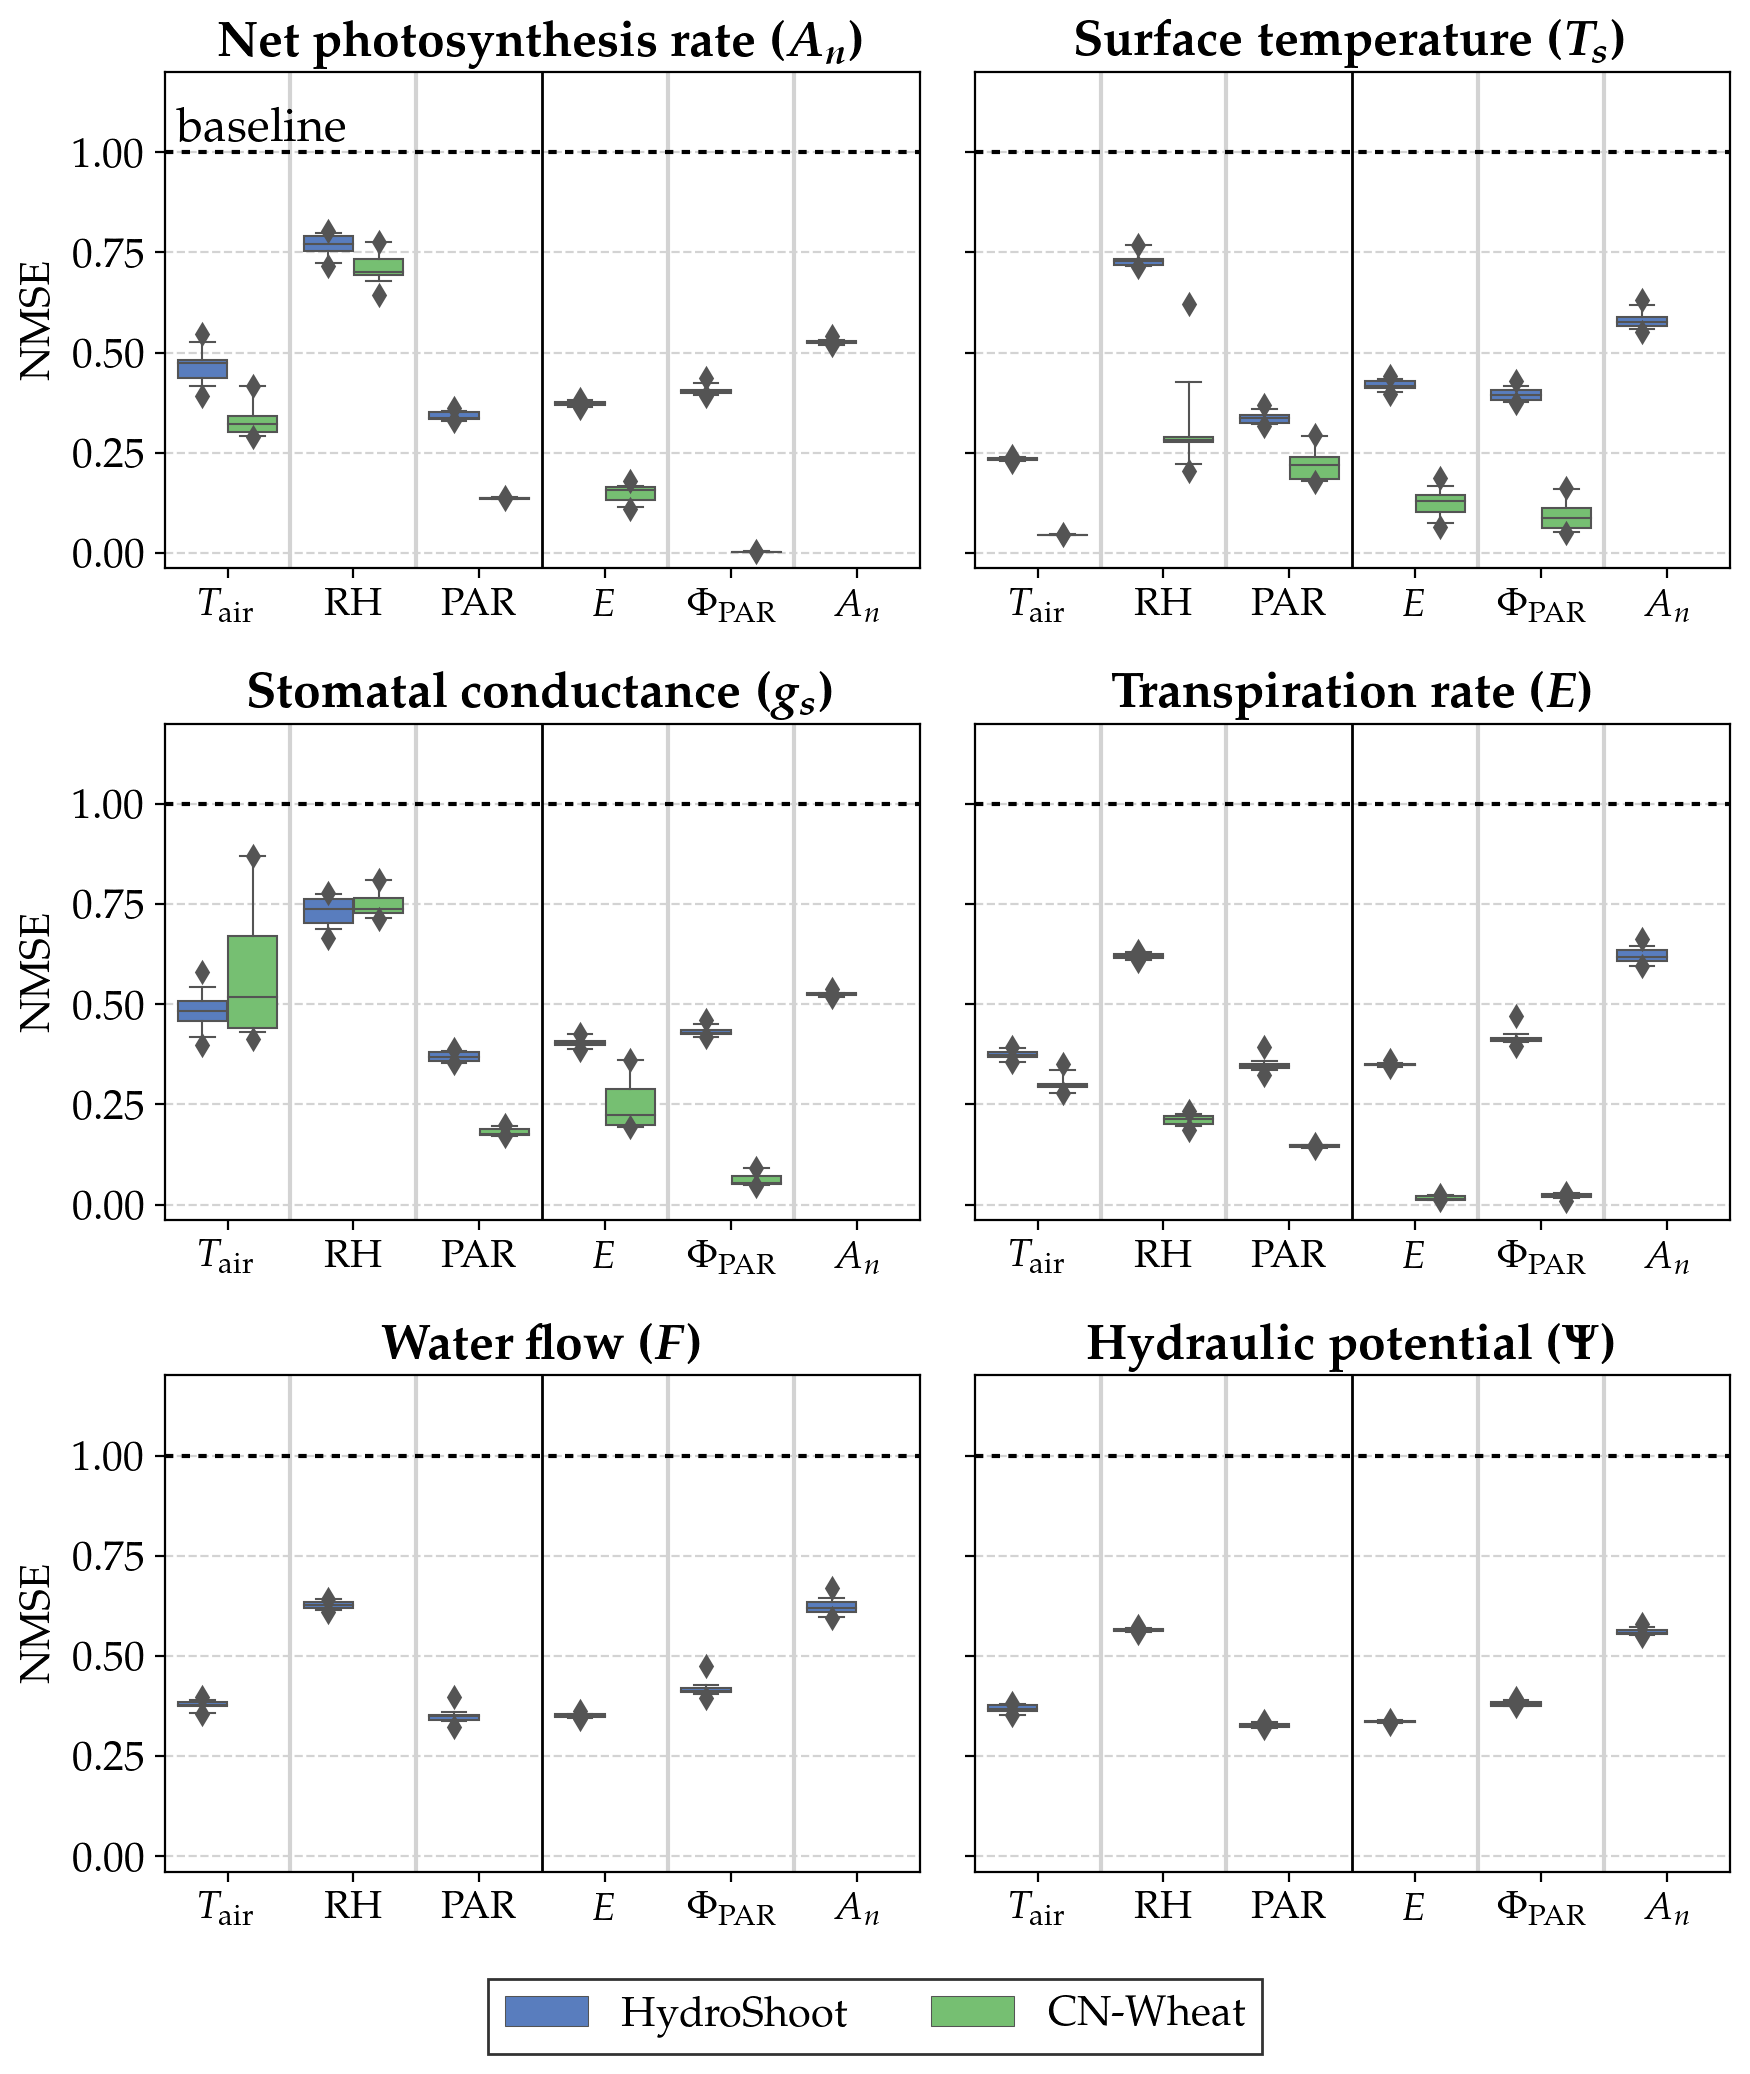
\includegraphics[width=0.82\textwidth]{img/regression_res_perf.png}
	\caption[Reservoir performance for input and physiological regression tasks.]
	        {Reservoir performance for input and physiological regression tasks.
	         The different plots show the prediction accuracy (y axis) for a suite of regression tasks (x axis) for each of the physiological reservoirs from \mbox{Table \ref{table:simulation_reservoirs}}.
	         The regression target of net photosynthesis rate  $A_n$ was only available for the HydroShoot model.
	         Each boxplot shows the distribution of test across 16 random reservoir samplings.
	         The box shows the quartiles of the distribution; the whiskers indicate the 5th and 95th percentiles.
	         Outliers are shown as a diamond shape.}
	\label{fig:input-phys-scores}
\end{figure}

% 	- *Caption:*
% 		- To measure the variance of the regression scores caused by the choice of observed plant elements, we used 16 random reservoir samplings and calculated
% - *Discussion boxplot figure:*
% - explanation of box plot whiskers etc.


% Regression predictions input and phys.
We study the time series prediction accuracy more closely in \mbox{Figure \ref{fig:predictions-input-phys}}.
In this figure, we see that the $E$ reservoir captures the broad dynamics of PAR and $\Phi_{\text{PAR}}$ for both HydroShoot and CN-Wheat.
However, HydroShoot cannot reproduce finer details, underpredicting the highest values and overpredicting the lowest values.
Moreover, the model's predictions sometimes lag behind the target (\mbox{Figure \ref{fig:predictions-input}}, samples A and C), other times the predictions lead the target (\mbox{Figure \ref{fig:predictions-input}}, sample D).
In contrast, CN-Wheat's transpiration rate captures finer details much better.

% Regression predictions input and phys.
\begin{figure}[hp]
    \begin{subfigure}[b]{\linewidth}
    	\centering
        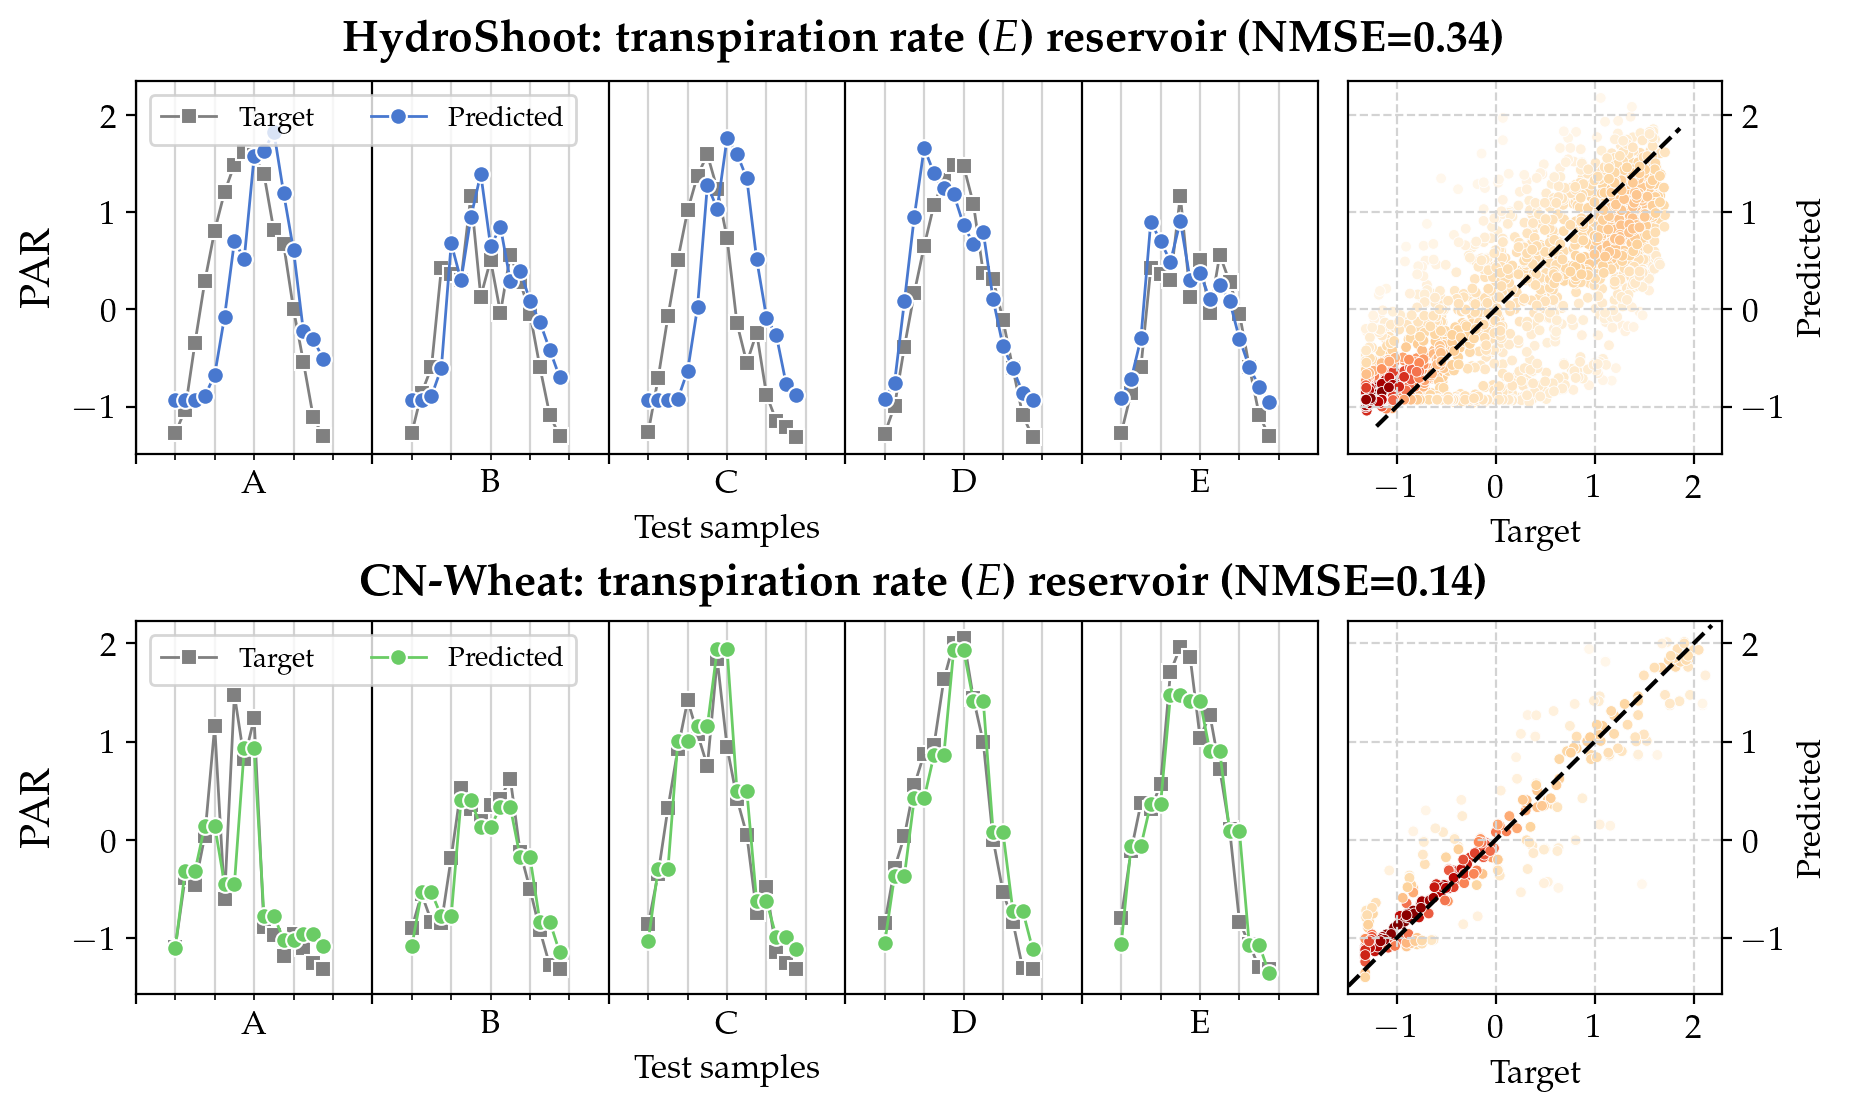
\includegraphics[width=\linewidth,keepaspectratio]{img/regression_res_prediction__input_PARi__state__Tr.png}
        \caption{Time series prediction of input PAR.}
    	\label{fig:predictions-input}
	\end{subfigure}
	\vskip\baselineskip
	\begin{subfigure}[b]{\linewidth}
	    \centering
        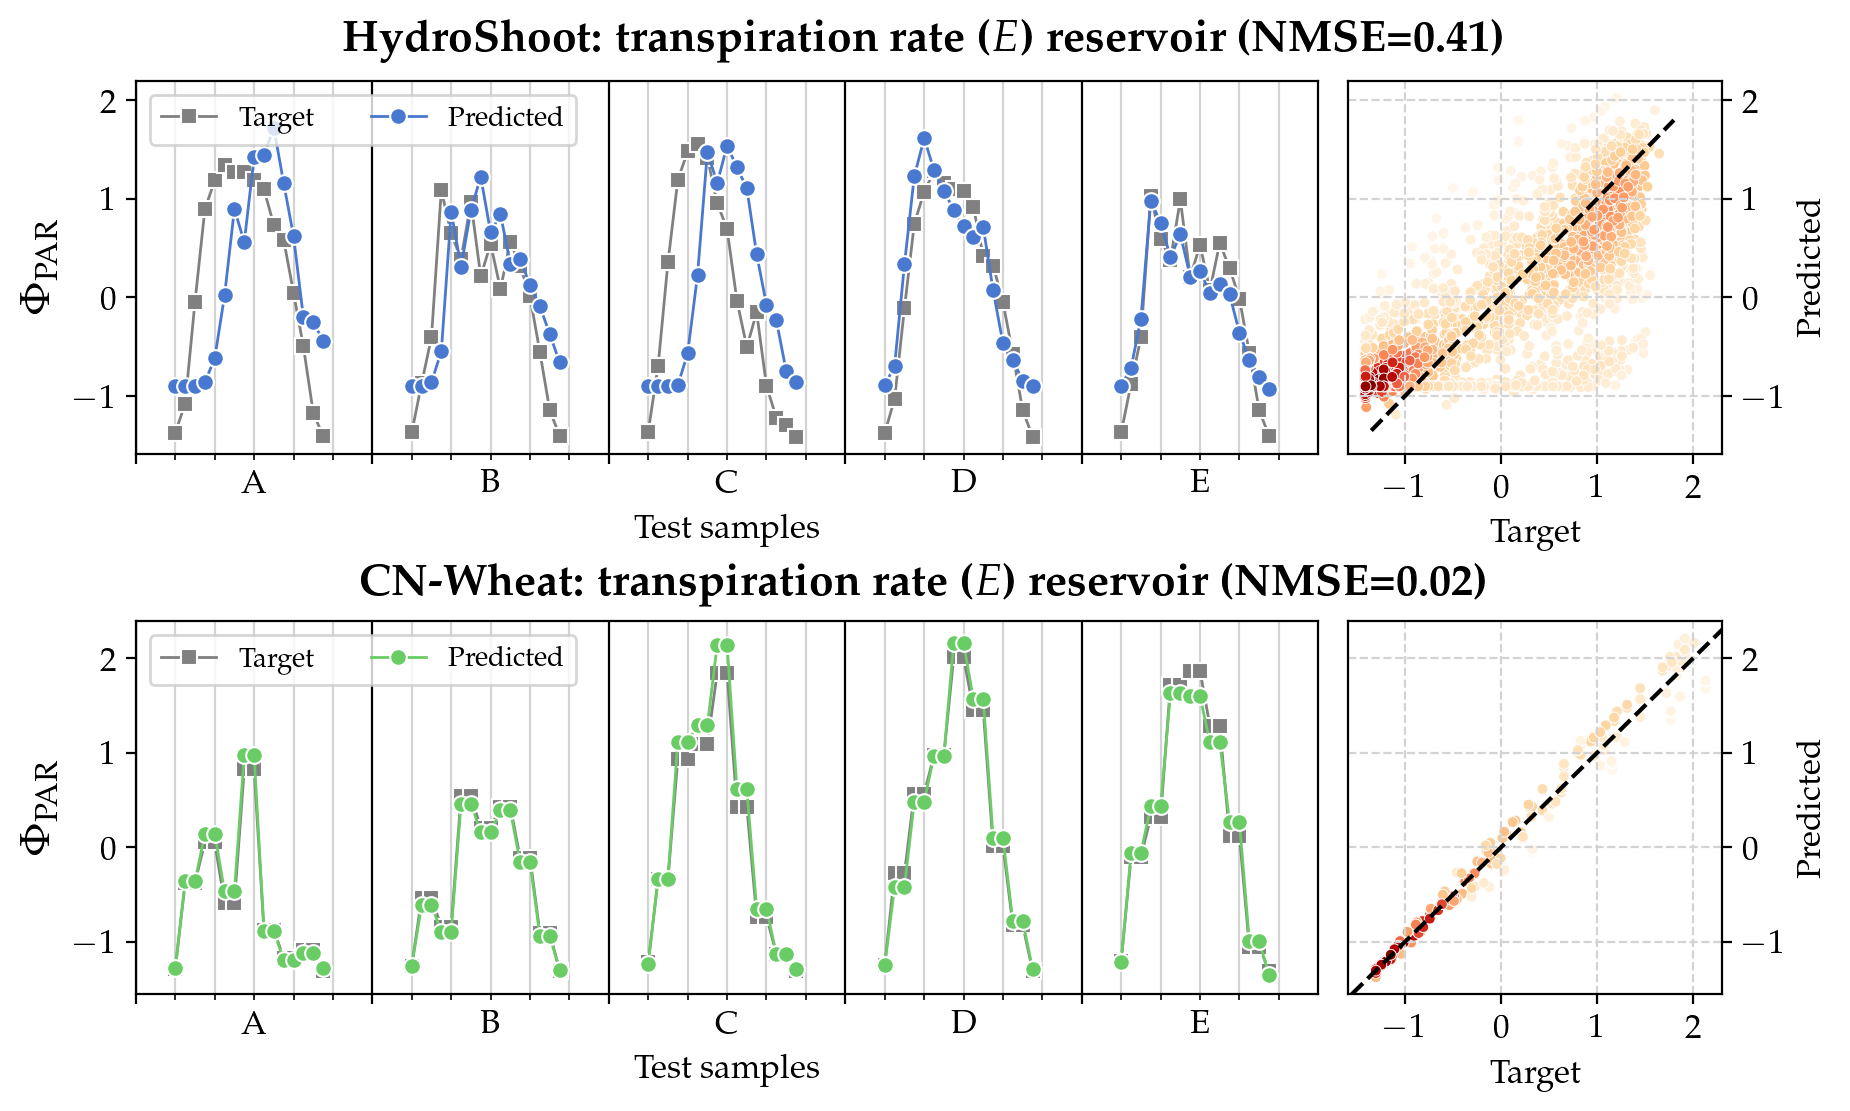
\includegraphics[width=\linewidth,keepaspectratio]{img/regression_res_prediction__output__custom__PARa__state__Tr.png}
        \caption{Time series prediction of absorbed PAR.}
    	\label{fig:predictions-phys}
	\end{subfigure}
	\caption[Time series prediction of input PAR and absorbed PAR using transpiration rate ($E$).]
	        {Time series prediction of input PAR and absorbed PAR using transpiration rate ($E$).
	         The left plot shows time series prediction for five random samples from the test set (see \mbox{Section \ref{sec:train-test-split}}),
	         the right shows the correlation between the target and predicted values. Darker colors indicate a greater density of points.}
	\label{fig:predictions-input-phys}
\end{figure}

% 	- *Caption:*
% 		- Left plots: time series prediction for five random samples from the test set (see Section 6.4).
% 		- Right plots: Correlation between target values and predicted values.
% 			- Points above the dashed line are overpredictions, points under it are underpredictions.


\subsection{Computational Benchmarks}

% Introduction
Next, we discuss the results for the computational benchmarks.
We present results for the delay line, polynomial expansion and \acrshort{narma} benchmarks based on two different input signals ($T_\text{air}$ and PAR).
For each benchmark, we compared the reservoir's advantage (or disadvantage) over a linear model of the input signal as we increased the benchmark's difficulty.
% we identified surface temperature ($T_s$) and transpiration rate ($E$) as the best performing reservoirs for these artificial tasks. 
In what follows, we discuss the results for the surface temperature ($T_s$) and transpiration rate ($E$) reservoirs specifically.


% Delay line performance of selected reservoirs
Figure \ref{fig:delay-line-scores} shows the results for the delay line benchmark.
Both reservoirs display memory capacity for solving this particular task.
For the $T_\text{air}$ input, one explanation for the observed memory is thermal inertia.
During the diurnal cycle, heat transfers between the air and the plant's water mass, which has a higher heat capacity than air.
This difference in heat capacity results in a slowed reaction to changes in ambient temperature.
The readout function can exploit this inertia to learn about past inputs.
Note that this is only a first-order interpretation, as it, for example, does not account for heat lost in evaporation.
A similar hypothesis can explain the results for incident PAR, as solar radiation affects the plant's temperature.
Lastly, we note that the transpiration rate shows similar performance characteristics as the surface temperature, indicating a possible relationship between the two processes.

\begin{figure}[t]
	\centering
    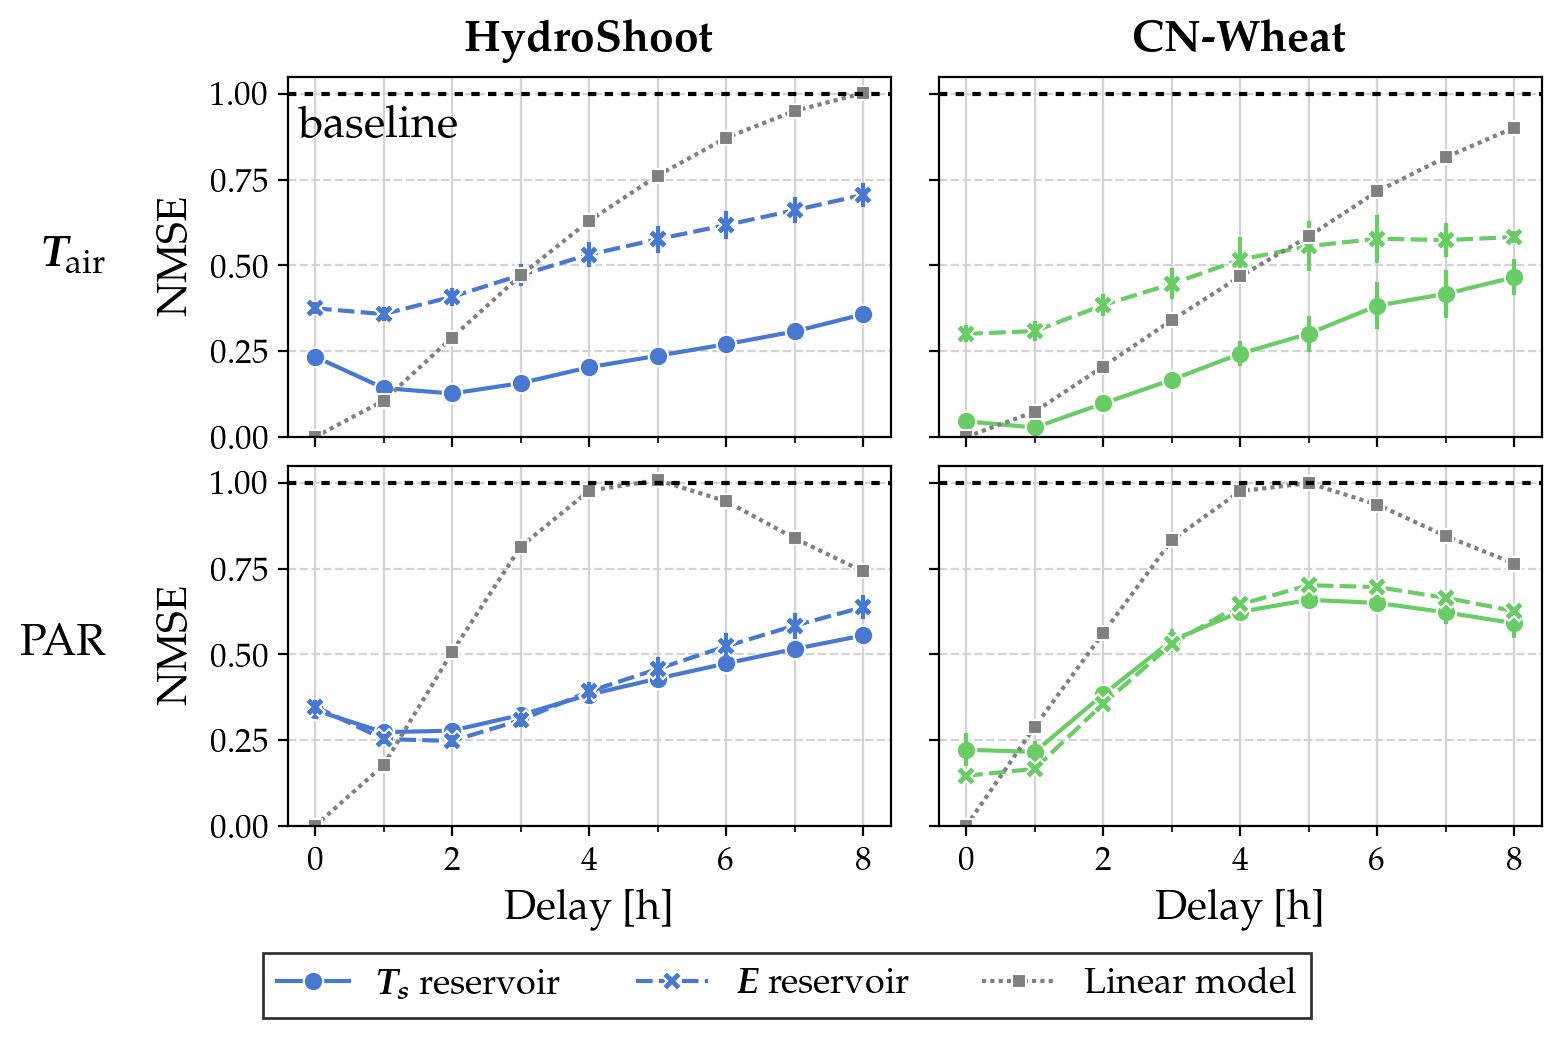
\includegraphics[width=0.82\textwidth]{img/comp_delay_perf.png}
	\caption[Predicting a time-delayed signal of $T_{\text{air}}$ and PAR using surface temperature ($T_s$) and transpiration rate ($E$).]%
    {Predicting a time-delayed signal of $T_{\text{air}}$ and PAR using surface temperature ($T_s$) and transpiration rate ($E$).
    In each plot, we compare the reservoirs' performance with a linear model that uses the benchmark's input as the only feature.
    The error bars show the scores' standard deviation.}

	\label{fig:delay-line-scores}
\end{figure}


% Polynomial task performance of selected reservoirs
Next, \mbox{Figure \ref{fig:poly-task-scores}} presents the accuracy predicting a polynomial expansion.
Interestingly, we observe a possibly polynomial relationship between the air temperature and the respiration rate, as the prediction error reaches a minimum for a degree of five.
For the other input-reservoir pairings, we see a similar performance characteristic as the linear model of the input signal, plus a bias penalty induced by the noisy relation between the reservoir and the input.

\begin{figure}[hp]
	\centering
    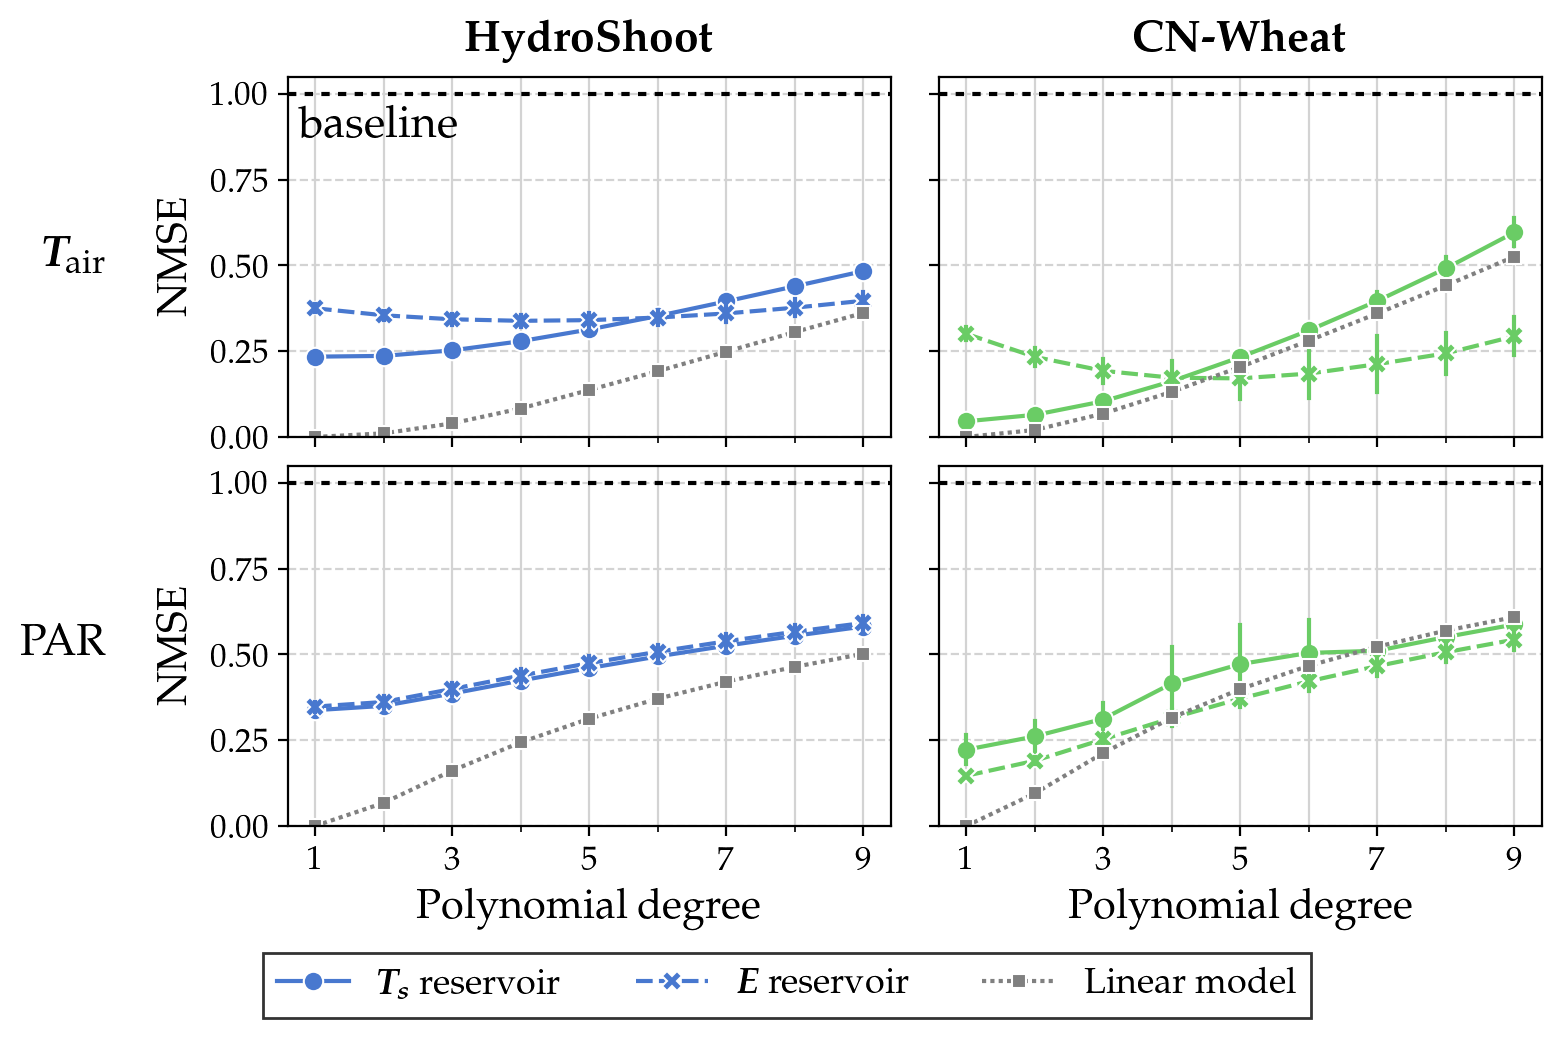
\includegraphics[width=0.82\textwidth]{img/comp_polynomial_perf.png}
	\caption%
	    [Predicting a polynomial expansion of $T_{\text{air}}$ and PAR using surface temperature ($T_s$) and transpiration rate ($E$).]%
	    {Predicting a polynomial expansion of $T_{\text{air}}$ and PAR using surface temperature ($T_s$) and transpiration rate ($E$).
	    In each plot, we compare the reservoirs' performance with a linear model that uses the benchmark's input as the only feature.
	    The error bars show the scores' standard deviation.}
	\label{fig:poly-task-scores}
\end{figure}


% NARMA benchmark performance of selected reservoirs
Finally, we consider the \acrshort{narma} benchmark.
In \mbox{Figure \ref{fig:narma-scores}} we increased the $n$ parameter from 2 up to 24. 
This means that, for $n=24$, the NARMA system integrates inputs from up to 24 hours in the past.
For the benchmark based on air temperature, only the $T_s$ reservoir outperformed the linear model. 
The same thermal inertia theory from the delay line task can explain this reservoir's correlation with this task.
Both surface temperature $T_s$ and transpiration rate $E$ outperform the linear model for the benchmark based on incident \acrshort{par}, particularly for $n$ values 8, 12, and 18.
The two reservoirs display similar performance for this task, further hinting at a relationship between the two.
From $n=18$ onwards, the performance of both the baseline model and the reservoirs improve over smaller values of $n$.
This can be explained as follows.
The input of the NARMA formula (\mbox{Equation \ref{prc:narma}}) has a period of twenty-four steps.
Setting $n=24$ means integrating over an entire day-night cycle in the formula.
This summation term then shows low variance as the input temperature and incident PAR have relatively constant cycles in our experiments (see the input data in \mbox{Appendix \ref{app:meteo}}).
The result is a smoothed, low-variance NARMA signal, which becomes easier to predict even with a linear model.
\mbox{Figure \ref{fig:predictions-narma}} shows the time series prediction for the NARMA8 task based on incident PAR, as predicted by surface temperature $T_s$.


\begin{figure}[hp]
	\centering
    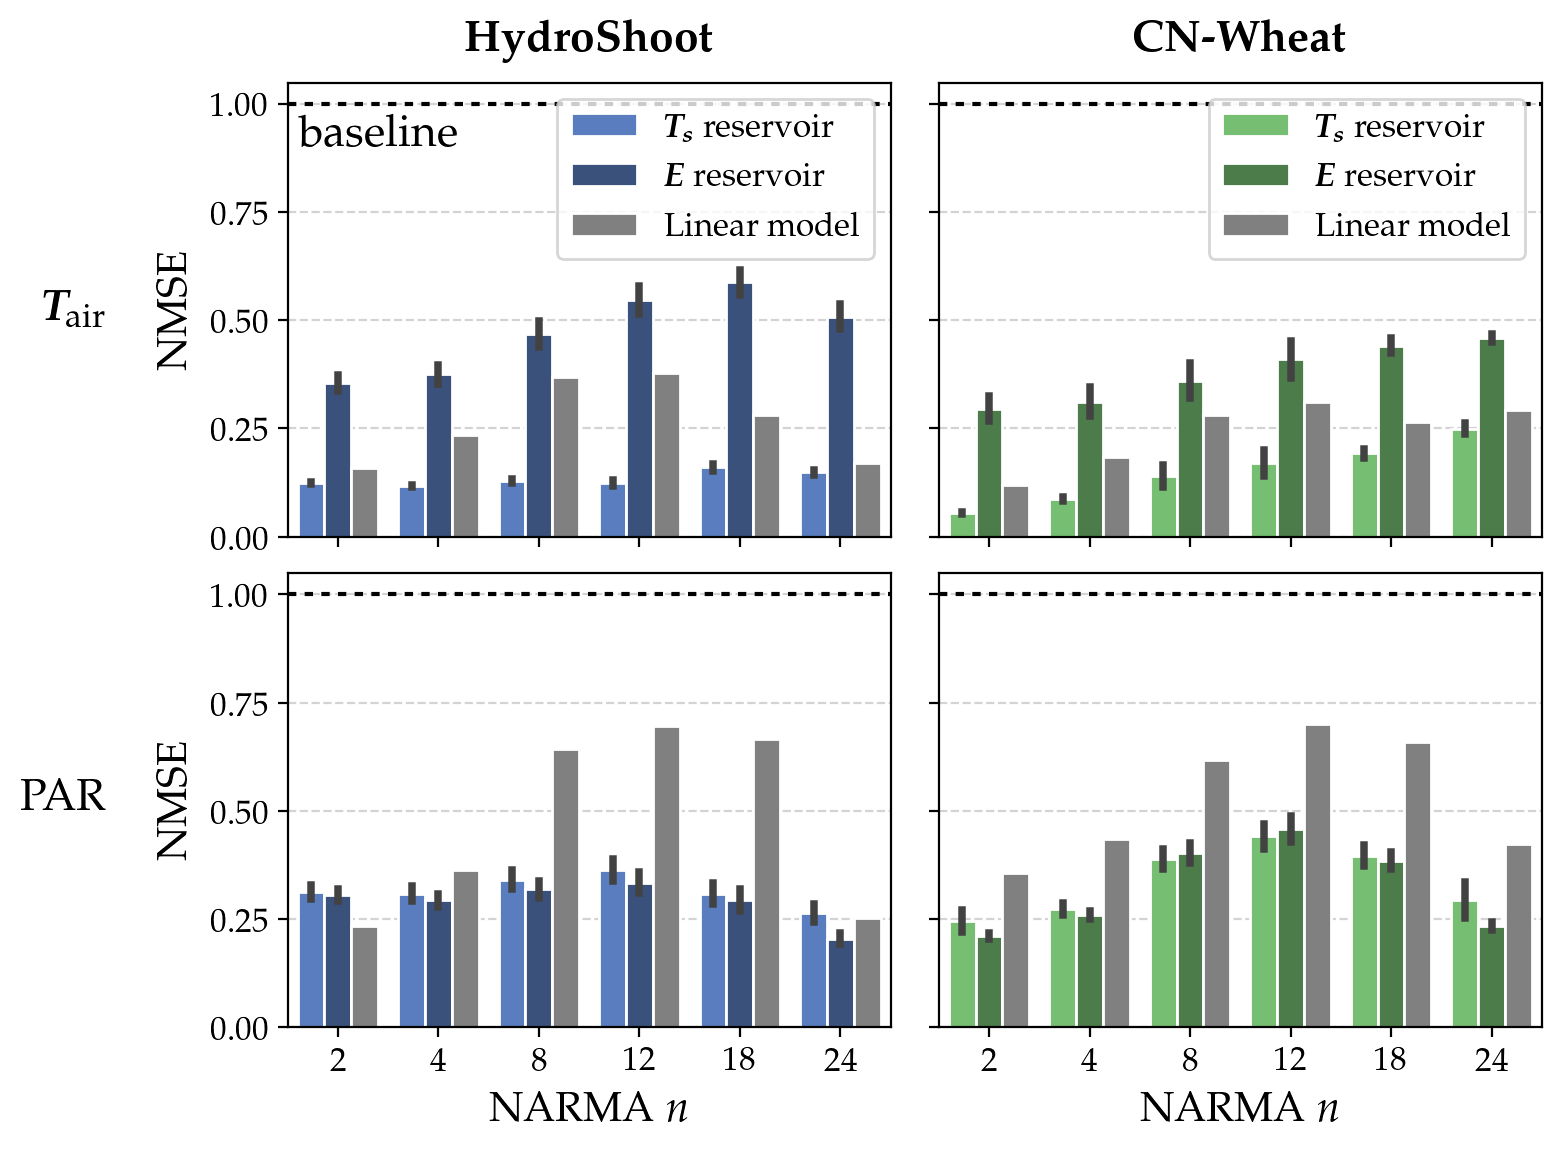
\includegraphics[width=0.82\textwidth]{img/comp_NARMA_perf.png}
	\caption[Predicting the NARMA benchmark based on $T_{\text{air}}$ and PAR using surface temperature ($T_s$) and transpiration rate ($E$).]%
	{Predicting the NARMA benchmark based on $T_{\text{air}}$ and PAR using surface temperature ($T_s$) and transpiration rate ($E$).
	In each plot, we compare the reservoirs' performance with a linear model that uses the benchmark's input as the only feature.
	The error bars show the scores' standard deviation.}
	\label{fig:narma-scores}
\end{figure}

% Regression predictions NARMA
\begin{figure}[hp]
	\centering
    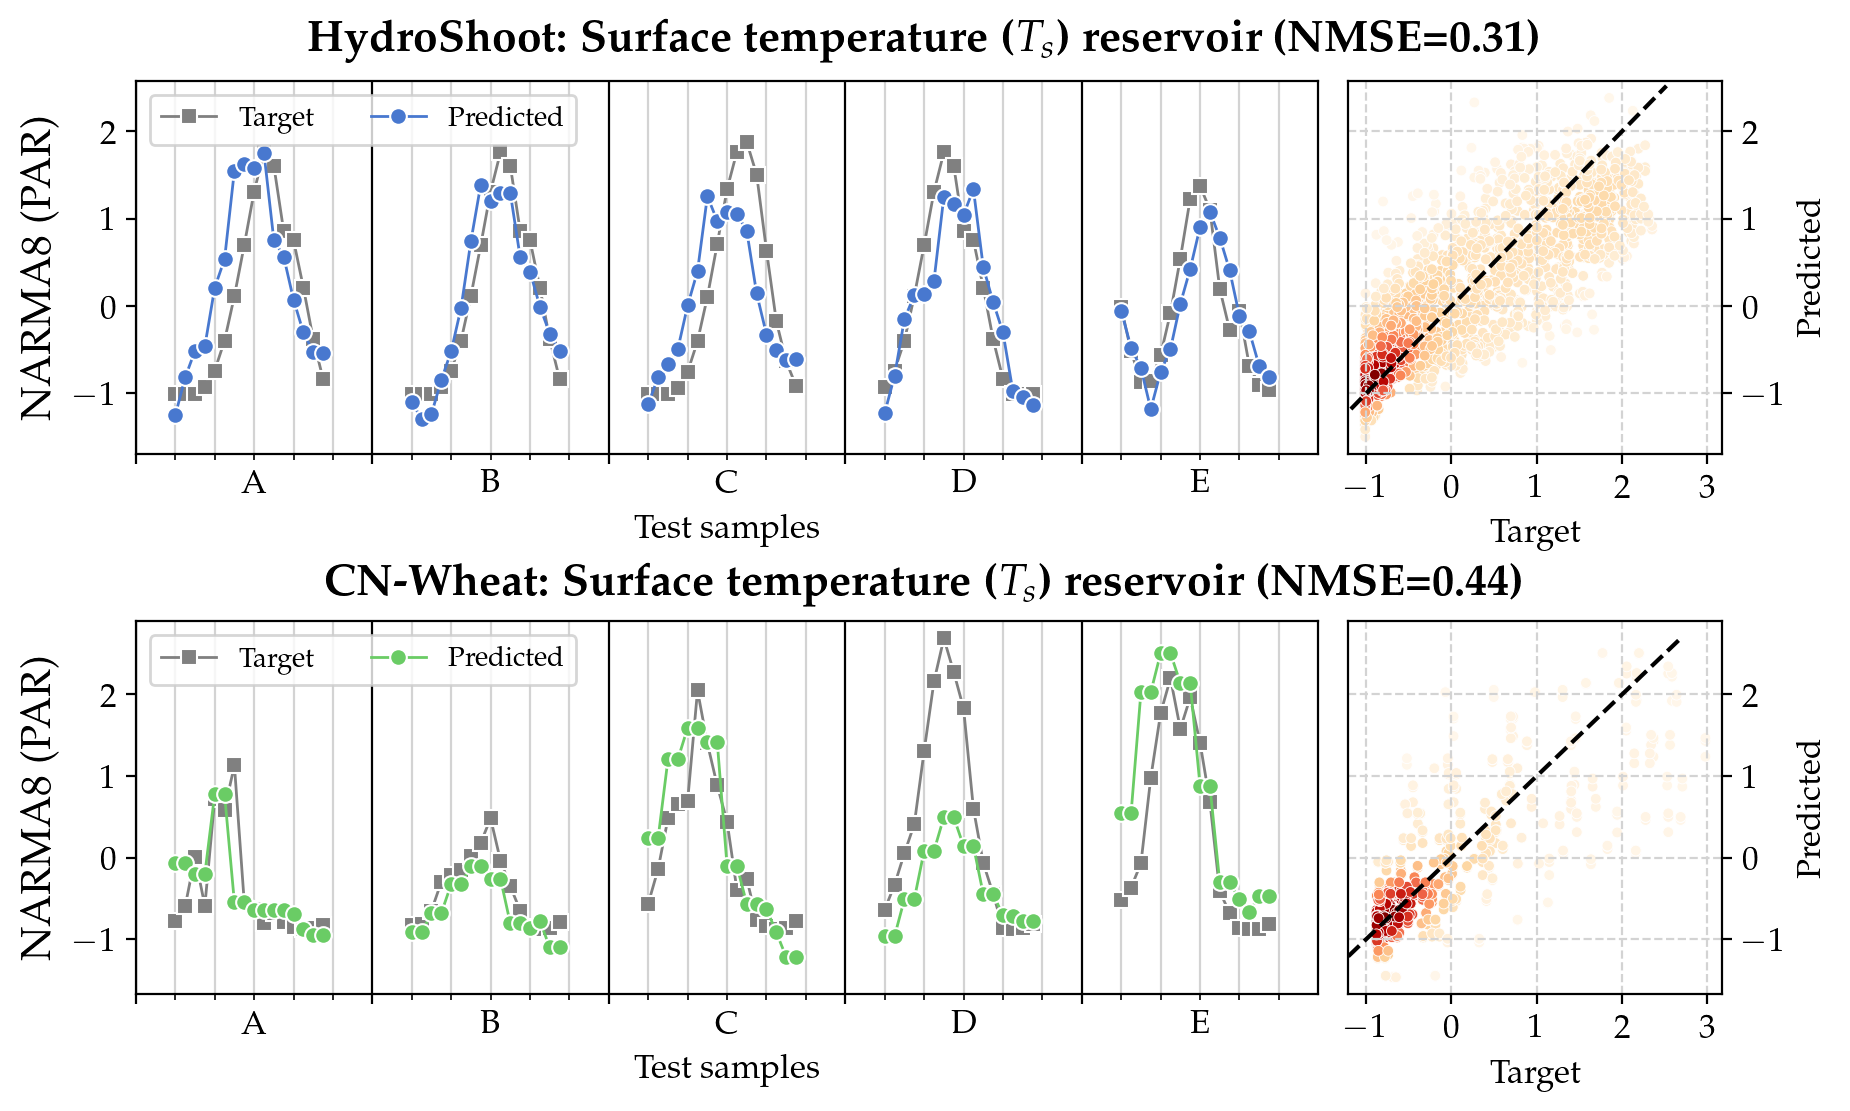
\includegraphics[width=\linewidth,keepaspectratio]{img/regression_res_prediction__input_PARi_NARMA_8__state__Ts.png}
    \caption[Time series prediction of the NARMA benchmark using surface temperature ($T_s$).]
        {Time series prediction of the NARMA benchmark using surface temperature ($T_s$).
        The left plot shows time series prediction for five random samples from the test set (see \mbox{Section \ref{sec:train-test-split}}),
         the right shows the correlation between the target and predicted values. Darker colors indicate a greater density of points.}
	\label{fig:predictions-narma}
\end{figure}

\subsection{Comparison with Previous Research}

% Comparison to Pieters 2022 results.
\citet{pieters_reservoir_2022} performed similar experiments using real-world strawberry plants.
His experiments used leaf thickness measurements of seven leaves as the observed reservoir, sampled every second.
Because leaf thickness strongly correlates with transpiration rate $E$ \citep{giuliani_coordination_2013}, we compare our results for the $E$ reservoir with the results reported using leaf thickness measurements.
We must emphasize that we are comparing prediction at different time scales; our models ran hourly, whereas Pieters' experiment was conducted at the second scale.

    The NMSE values we obtained for the input and physiological tasks are in line with what is reported by Pieters, with HydroShoot performing a bit worse and CN-Wheat a bit better than what was reported for the strawberry plant.
HydroShoot performed notably worse at predicting $E$ and $A_n$ than the strawberry plant.
However, in terms of reservoir observability, Pieters' experiment aligns closer with our reservoir for CN-Wheat than for HydroShoot.


Pieters used incident PAR as a base for the computational benchmarks, so we compare our results for that input.
We obtained significantly better results for the polynomial tasks.
The strawberry plant's prediction accuracy capped out at an NMSE of nearly 1.0 for only a degree of 6, whereas our \textit{in silico} plants achieve NMSE scores under 0.6 for up to a degree of 9.
However, our baseline linear model also performed better than Pieters' control experiment, suggesting there may be a difference in methodology that makes the tasks complicated to compare. 
The data for the delay line task can be compared for delays of 1-5 \unit{\hour}. 
Here, the results obtained in our experiments are similar to those observed for the strawberry plant.
The results for the NARMA benchmark are more difficult to compare because The NARMA task used in Pieters' work operated at the minute scale, using the alternative formulation from \mbox{Equation \ref{prc:narma-timescale-adapted}} with $\tau=60$.
Because of the hourly time step in our plant models, we designed our NARMA task at the hour scale (i.e.\ with $\tau=1$).
% The NARMA task used in Pieters' work operated at the minute scale, i.e.\ $n=100$ integrates inputs up to 100 minutes in the past.
% Because of the limited time resolution of our plant models, we designed our NARMA task at the hour scale.
We obtained significantly better results with our version of the benchmark than were reported for the minute scale task; 
The strawberry plant did not achieve NMSE values lower than 0.5 for any NARMA task.
As we explained in the previous section, this disparity may be because the NARMA task at the hour scale results in a more smoothed signal.

\section{Fading Memory}

To test the fading memory principle, we applied an impulse of varying length and amplitude to the incident \acrshort{par} of each plant model.
The experiment revealed unexpected properties in the \acrshort{fspm}s.
\mbox{Figures \ref{fig:result-impulse-cnwheat}} \mbox{and \ref{fig:result-impulse-hydroshoot}} show the divergence $\delta(t)$ (Equation \ref{methods:reservoir_divergence}) in each physiological process caused by the impulse for CN-Wheat and HydroShoot respectively.

\subsection{CN-Wheat}

Let us first study the effects of the artificial stimulus on CN-Wheat (Figure \ref{fig:result-impulse-cnwheat}).
It is immediately apparent that the reservoir's divergence changes at intervals of two hours instead of the hourly steps of the inputs.
Indeed, \citet{barillot_cn-wheat_2016-1} confirms that some submodels of CN-Wheat run at two-hour intervals to limit computational cost.
The figure indicates that the affected submodels control each of our physiological reservoirs.
On the one hand, this is unfortunate because, for our use case, the practical simulation scale is \SI{2}{\hour} instead of \SI{1}{\hour}.
On the other hand, even at this coarser simulation scale, the model was able to perform tasks well at the \SI{1}{h} scale in Section \ref{results:input-sep}. Perhaps, the results could be even more promising when simulated with an hourly time step.

Because we chose the impulse lengths to be odd, we see some misalignment between the impulse steps and the steps that show disturbance in the reservoir.
Looking past the misalignment caused by the \SI{2}{\hour} simulation interval, we see that the reservoir divergence immediately disappears when the real input signal resumes.
The most likely explanation is that the transient behavior lasts less than two hours, such that the coarse simulation steps mask any memory effects.
An alternative explanation is that the FSPM's state is a memoryless function of the immediate environmental conditions. 
We think this is unlikely because the plant model should be dynamic by construction.
We also reject the explanation that the impulse is too short to impact the reservoir because we see the same behavior resulting from a \SI{1}{\hour} or \SI{9}{\hour} stimulus.
Either way, we can safely conclude that all reservoirs in the CN-Wheat model show stationary behavior w.r.t. the PAR input as their dynamics resumed as if the impulse did not occur.

At first glance, these results for CN-Wheat seem to contradict the behavior we saw in Figure \ref{fig:delay-line-scores} for the delay line task.
We saw that $T_s$ and $E$ can predict past incident PAR better than a linear baseline model (though the scores are overall still quite bad).
An alternative explanation for this performance is that the \SI{2}{\hour} simulation steps add memory of the past hour to the reservoir for every second time step.
Figure \ref{fig:delay-line-scores} supports this theory: the reservoirs display near-identical prediction accuracy for delays of 0 h and \SI{1}{\hour} before sharply increasing for a delay of \SI{2}{\hour}.

\begin{sidewaysfigure}[hp]
	\centering
    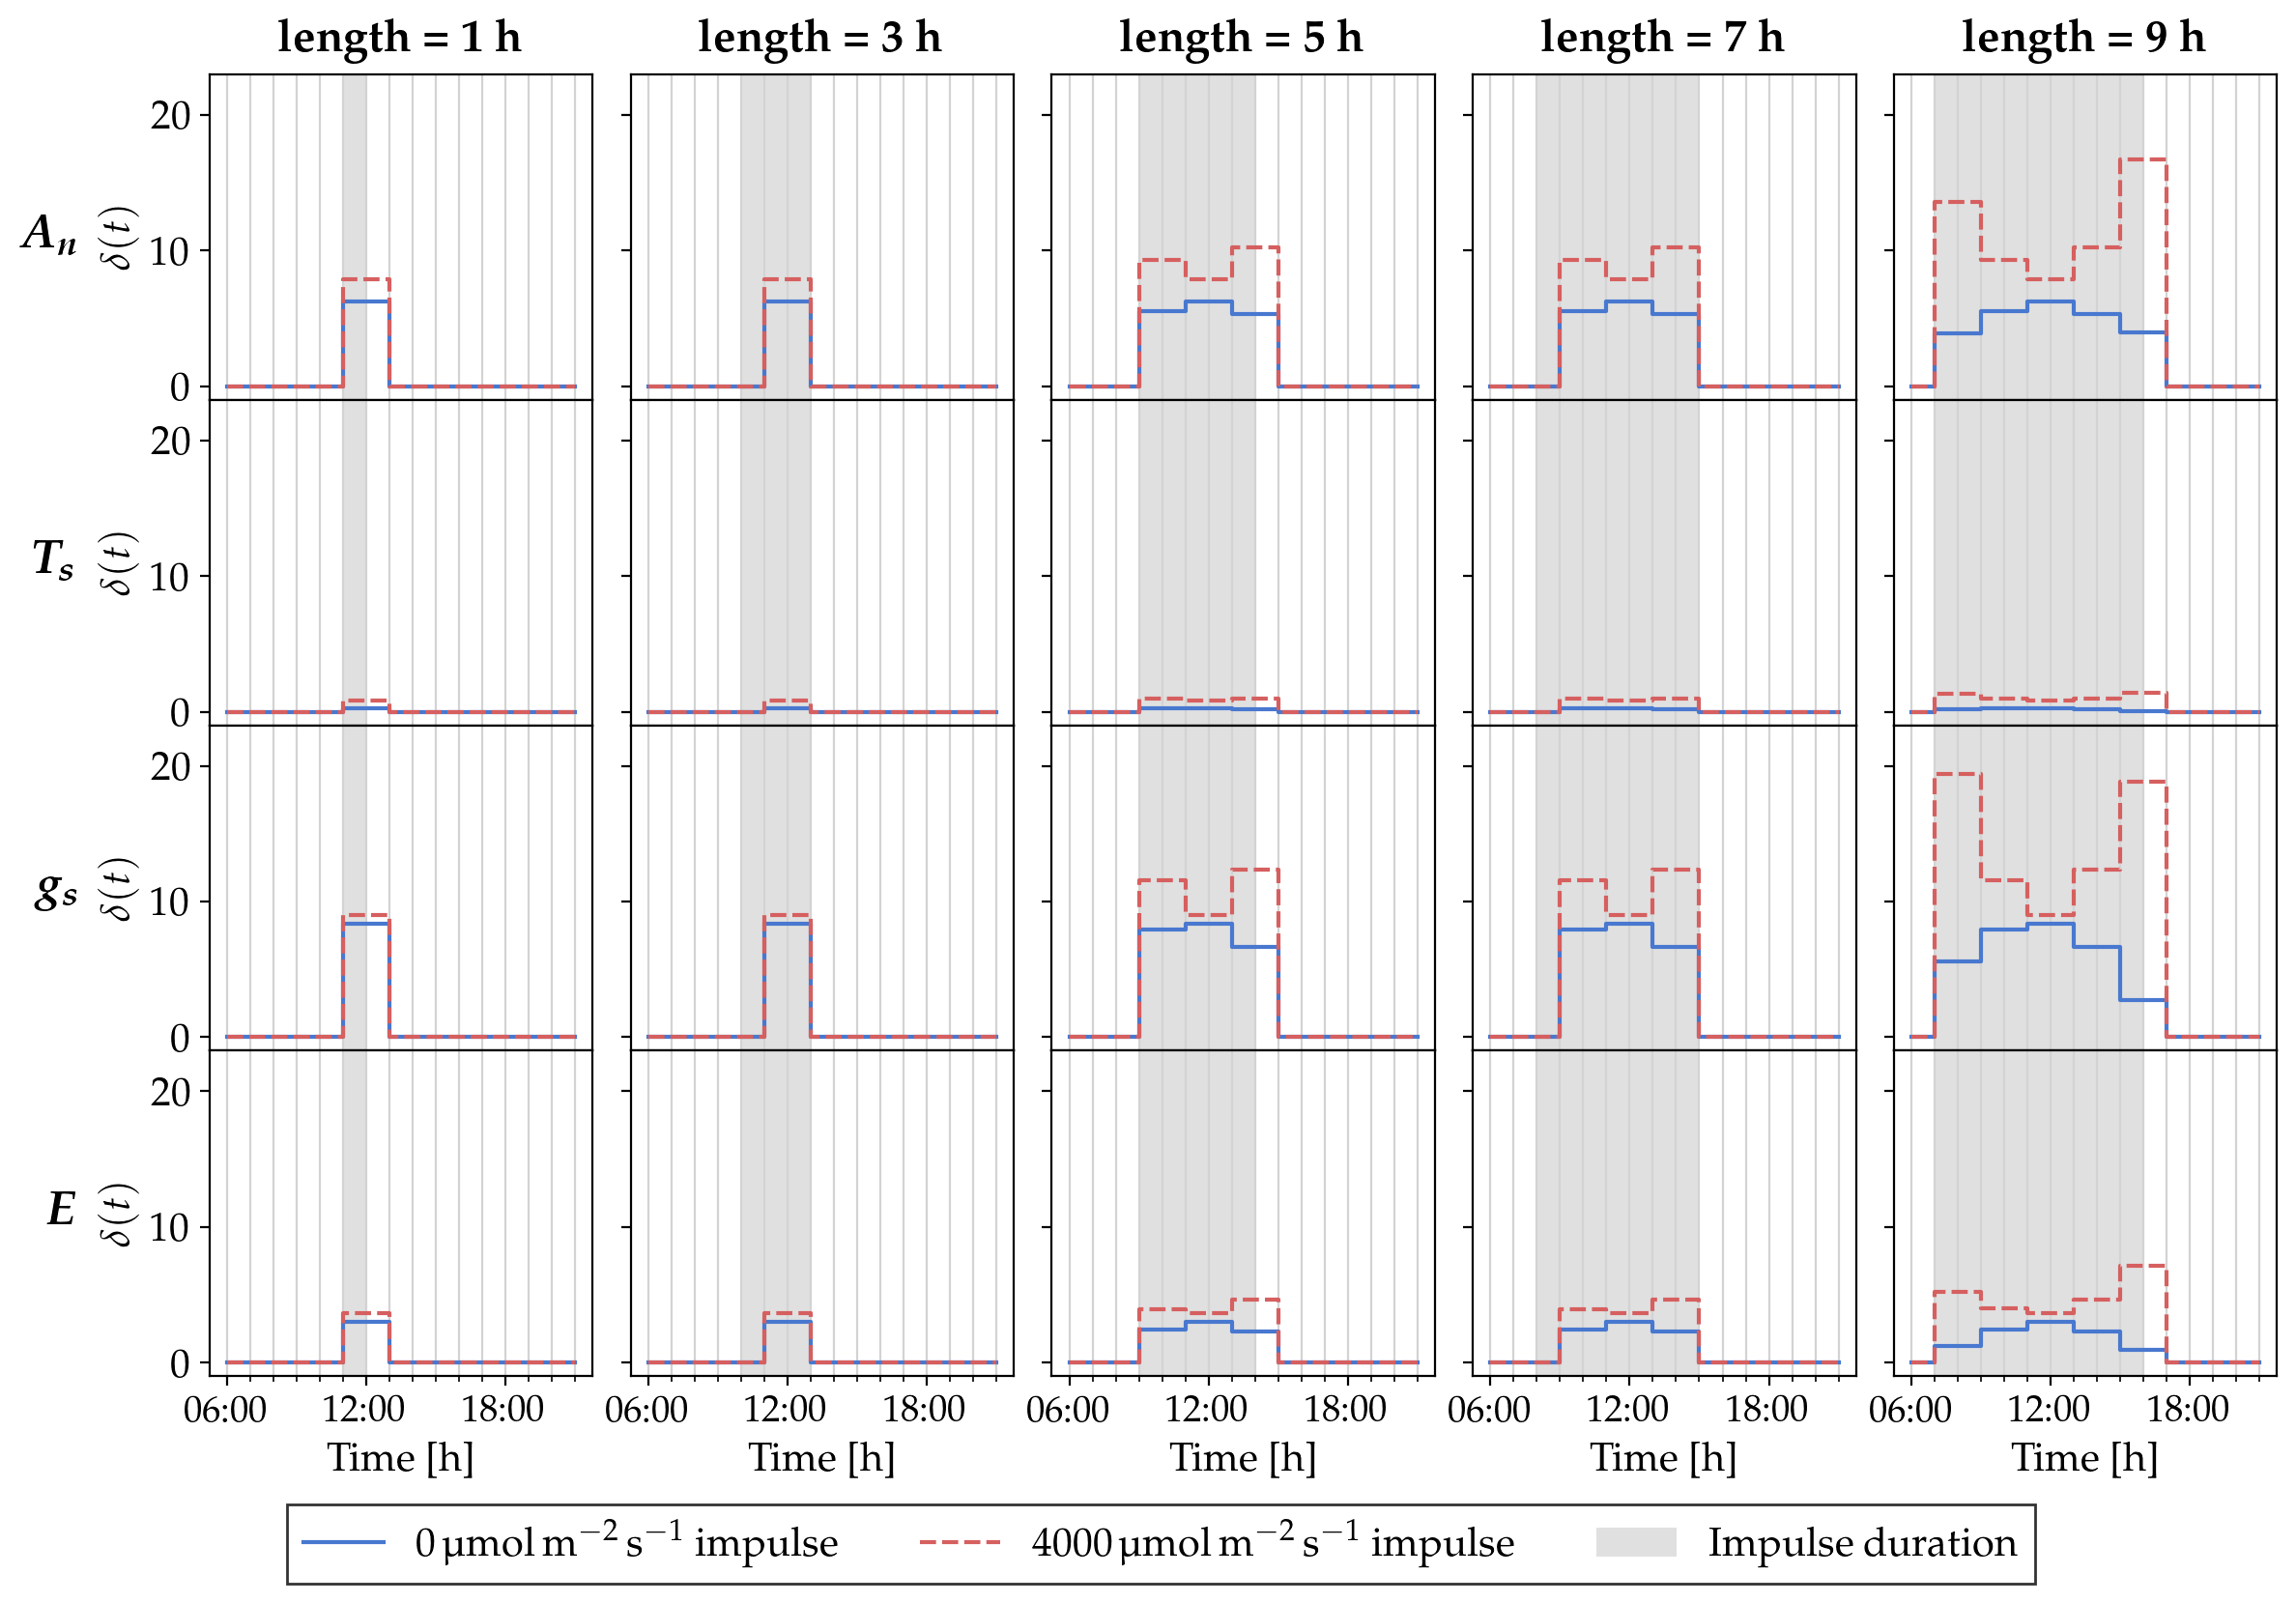
\includegraphics[width=20cm]{img/impulse_reservoirs_cnwheat.png}
	\caption{
	    CN-Wheat: Reservoir divergence $\delta(t)$ (Equation \ref{methods:reservoir_divergence}) after applying an impulse to PAR of various lengths and amplitudes.
    }
	\label{fig:result-impulse-cnwheat}
\end{sidewaysfigure}


\begin{sidewaysfigure}[hp]
	\centering
    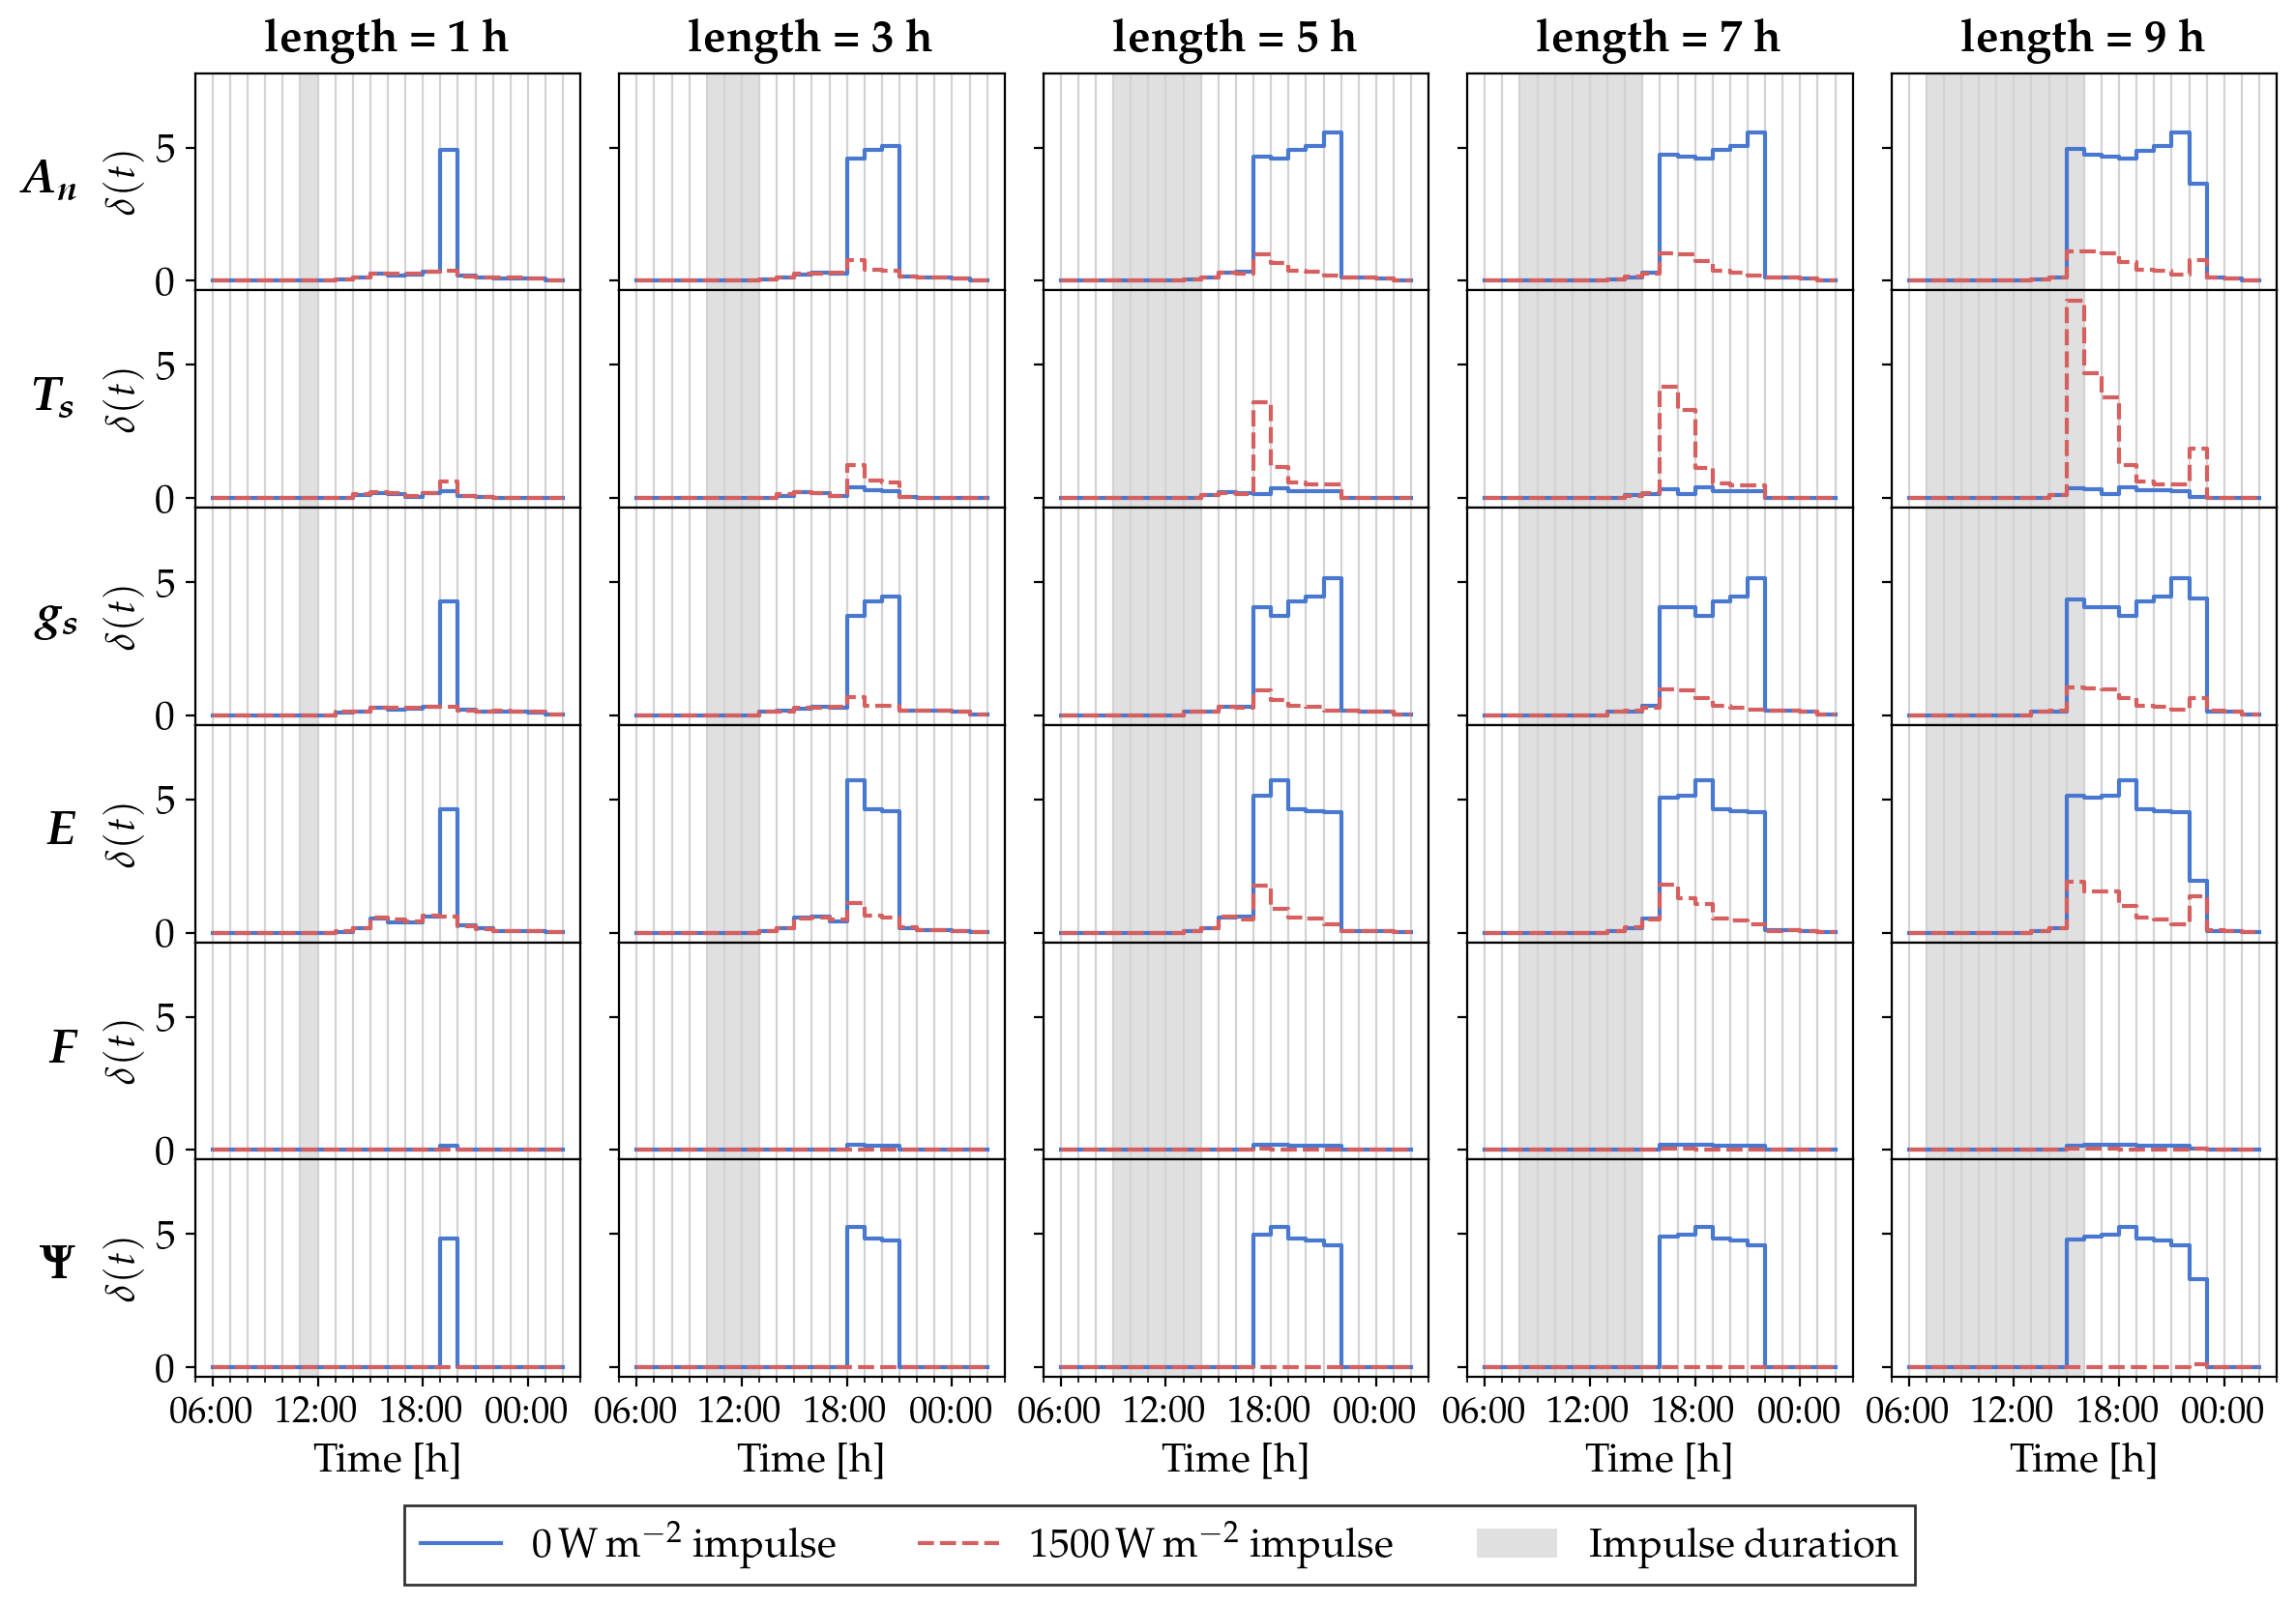
\includegraphics[width=20cm]{img/impulse_reservoirs_hydroshoot.png}
	\caption{
	    HydroShoot: Reservoir divergence $\delta(t)$ after applying an impulse to PAR of various lengths and amplitudes.
    }
	\label{fig:result-impulse-hydroshoot}
\end{sidewaysfigure}


\subsection{HydroShoot} \label{sec:results-impulse-hydroshoot}

% Hydroshoot discussion (1)
Next, we discuss the outcome of the impulse experiment for the HydroShoot \acrshort{fspm}.
Figure \ref{fig:result-impulse-hydroshoot} shows that the disturbance in the reservoir caused by the impulse in incident PAR lasts for the same length as the applied stimulus. However, the reservoir reacts at an \SI{8}{\hour} delay.
We first investigate this delayed reaction before drawing further conclusions from this data.


% Hydroshoot stability discussion (chaotic behavior)
Figure \ref{fig:hydroshoot-instability-divergence} shows the divergence metric for the entire simulation duration and compares various experimental setups.
Note that each experiment had identical initial conditions and experienced identical environmental conditions up to the start of the impulse on day 5.
The plot shows that the reservoir dynamics diverge slightly during daytime even under identical conditions.
This indicates that the observed physiological processes display somewhat chaotic dynamics during daytime hours.
Keep in mind that this cyclical divergence is quite low compared to the disturbance caused by the impulse ($\delta(t)$ of 0.4 vs. 3.5 in \mbox{Figure \ref{fig:hydroshoot-instability-divergence}}).
We did not observe cyclical divergence in CN-Wheat.
The chaotic behavior may be a result of numerical instabilities in the simulation.
However, previous reports of chaotic behavior in plant physiological processes exist in the literature.
For example, \citet{shabala_observations_1997} reported chaotic dynamics in plant physiological responses to light, which aligns with our observations.
Therefore, the chaos observed in HydroShoot may be a more realistic model than the deterministic behavior of CN-Wheat.


% Hydroshoot stability discussion (delayed responses)
Another anomaly in the HydroShoot simulation is shown in Figure \ref{fig:hydroshoot-instability-behavior}.
The figure shows a superposition of the input PAR and the mean transpiration rate of the observed reservoir elements.
The data reveals a continuously shifting misalignment between the diurnal cycle of the input signal and the oscillations in the physiological dynamics.
In an extreme example, the peak in transpiration rate lags nearly a half-period behind the incident PAR on day 4.
Comparing this data to Figure \ref{fig:hydroshoot-instability-divergence} reveals that the cyclical peaks in reservoir divergence we discussed earlier are aligned in time with these time-shifted reservoir responses.
We observed this behavior for any simulation starting day.
We were unable to identify the root cause for these dynamics, and the CN-Wheat model did not exhibit similar behavior.
This anomaly may also explain the leading and lagging predictions we observed in Figure \ref{fig:predictions-input-phys}.


% Hydroshoot discussion cont'd (2)
Continuing the analysis of the experimental results: the shifting delay in reservoir response is the most likely explanation for the delayed response to the artificial stimulus.
Since we know of the chaotic response to incident light, we must attribute the slight disturbance that precedes the delayed peak in reservoir divergence to the natural chaotic behavior and not the impulse.
Because the peak in disturbance has the same duration as the impulse and accounting for the assumed delay in reaction of \SI{8}{\hour} in the reservoir's response, we cautiously propose the same conclusion as for CN-Wheat.
That is, no lasting memory effects are visible at the simulation scale of \SI{1}{\hour}; if there are any transient dynamics, they must occur over a much shorter time frame.

% Regression predictions input and phys.
\begin{figure}[hp]
    \begin{subfigure}[b]{\linewidth}
    	\centering
        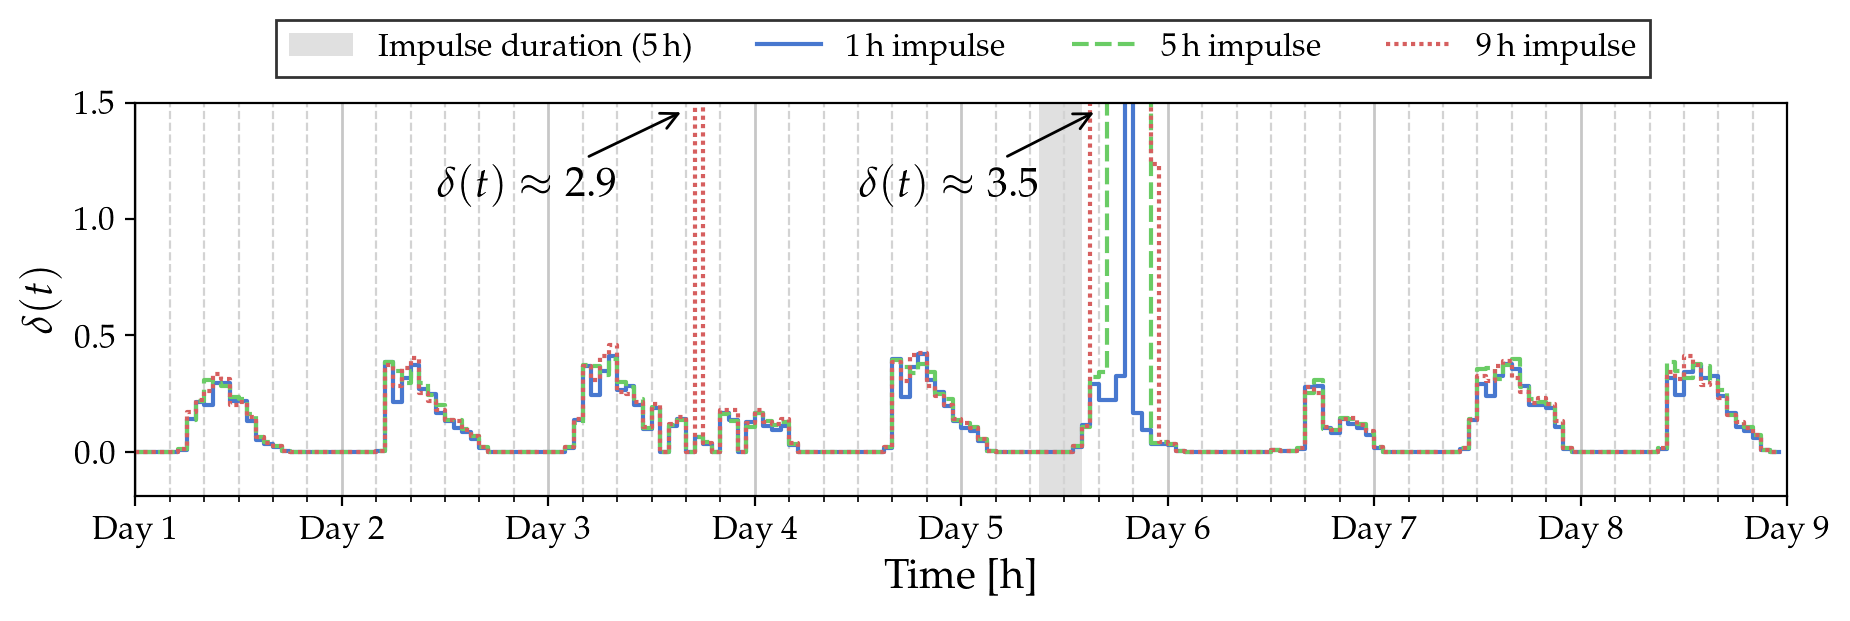
\includegraphics[width=\linewidth,keepaspectratio]{img/hydroshoot_instability_divergence.png}
        \caption{HydroShoot: Reservoir divergence $\delta(t)$ in various experiments with impulse amplitude \SI{0}{\watt\per\square\meter}.}
    	\label{fig:hydroshoot-instability-divergence}
	\end{subfigure}
	\vskip\baselineskip
	\begin{subfigure}[b]{\linewidth}
	    \centering
        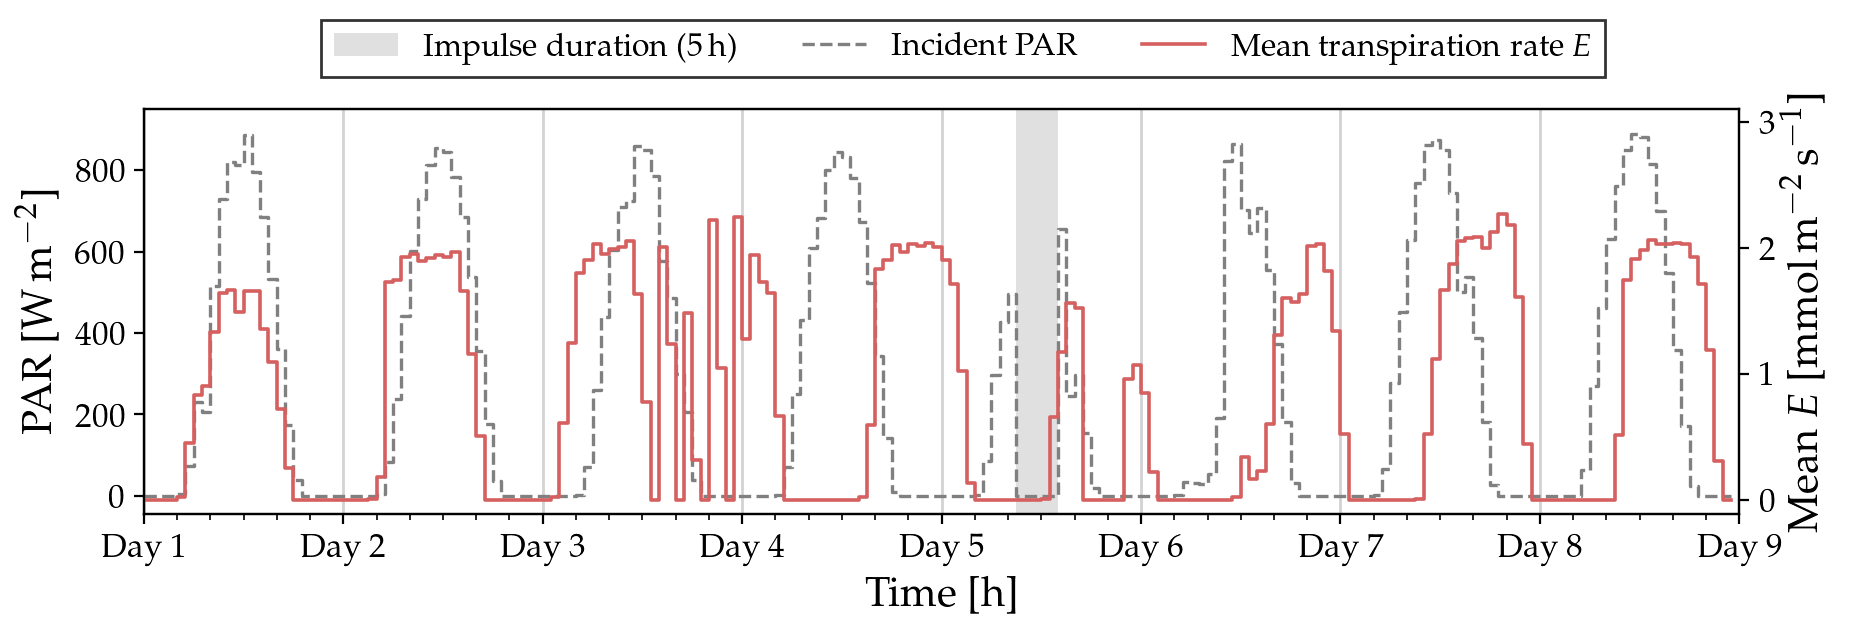
\includegraphics[width=\linewidth,keepaspectratio]{img/hydroshoot_instability_behavior.png}
        \caption{HydroShoot: Input data and modeled transpiration rate from an impulse experiment with length \SI{5}{\hour}.}
    	\label{fig:hydroshoot-instability-behavior}
	\end{subfigure}
	\caption[Two figures highlighting unstable behavior observed in the HydroShoot \acrshort{fspm}.]
        	{Two figures highlighting unstable behavior observed in the HydroShoot \acrshort{fspm}.
        	(\subref{fig:hydroshoot-instability-divergence}) 
	            Reservoir divergence $\delta(t)$ in various experiments with impulse amplitude \SI{0}{\watt\per\square\meter}.
                Under all circumstances, a cyclical pattern of reservoir divergence emerges.
        	(\subref{fig:hydroshoot-instability-behavior}) 
        	    Input data and modeled transpiration rate $E$ from an impulse experiment with length \SI{5}{\hour}.
        	    The superposition of the data reveals a shifting misalignment between the diurnal pattern of incident PAR and the consequent transpiration rate.
        	}
	\label{fig:hydroshoot-instability}
\end{figure}



% **Weaknesses:**
\section{Weaknesses in Our Methods and Potential Improvements}

% In the spirit of academic honesty, we must point out the weaknesses in our methods too.
We can identify some potential weaknesses that may have influenced our results.
For one, we used the same measurements for the reservoir as are used by the model to compute the physiological regression tasks.
This introduces positive bias into the correlation between the reservoir and the physiological targets.
This bias is especially pronounced in the accuracy of CN-Wheat for predicting total transpiration rate and absorbed PAR; 
the readout model has a distinct advantage because it could directly observe 70\% of the plant's internals.
To reduce this bias, we could have introduced some signal noise to the observations to make them less precise.
However, it is difficult to determine what amount of noise is appropriate in this case.

Another weakness is the trust we placed in the accuracy of the used FSPMs.
The authors of these plant models have only validated their accuracy for the use cases presented in their publications.
Plant models are generally not verified as one hundred percent accurate copies of their real-world counterparts.
As we observed in Section \ref{sec:results-impulse-hydroshoot}, the HydroShoot model showed some unexpected behavior that was not reported in the original paper.
To emphasize that our results characterize the behavior of plant models and not live plants, we used the names of the FSPMs throughout this chapter instead of the plant genus. 

Finally, the lack of time resolution in the plant simulations leaves us with a weak take-away about transient memory dynamics in the studied plant species.
Though we can conclude that the considered physiological reservoirs show stationary behavior at the hour scale, we cannot state the exact period for which past inputs influence the present reservoir dynamics.



\section{Summary}

In this chapter, we demonstrated the use of eco-physiological processes in computer plant models for reservoir computing.
Our results for regression tasks highlighted several promising processes that showed good predictive correlation with biologically relevant tasks.
The results can be used in future plant \acrshort{rc} research to decide which physiological processes to pursue.
The impulse experiment was less conclusive.
However, the initial results seem to imply that each considered reservoir has fading memory that lasts less than two hours, with regards to incident \acrshort{par}.
The difficulties in using the selected \acrshort{fspm}s for this experiment highlighted the need for plant models with a better time resolution than \SI{1}{h}.
Finally, through our analysis of reservoir dynamics, we observed chaotic characteristics of eco-physiological processes, as well as unexpected behavior in a plant model that was previously unreported.
Because the application of \acrshort{rc} was able to reveal these behaviors in plant models so readily, we propose that \acrshort{rc} can play a more prominent role not only in plant computation but also in the development and verification of \acrshort{fspm}s.

\chapter{Conclusion} \label{chapter:discussion}

% **Introduction:**
The previous chapter reported the quantitative results of our experiments along with our interpretation of the data and a discussion of their implications.
This chapter offers broader conclusions to the experiments we conducted.
% We also point out potential weaknesses in our experimental setup and how they could be mitigated in future work.
Then, we briefly recap the weaknesses we found in mechanistic plant models and how they can be improved.
Finally, we propose a few directions for future research and potential applications of plant RC.


% **Results implications:**
\section{Implications of the Results}

Our experiments showed promising results for plant RC with several plant physiological processes.
% We observed similar results for each of the processes we considered.
To pick reservoirs for future research, we recommend cross-referencing our results of reservoir performance with available sensing technologies to select the physiological reservoir with the highest potential.
For example, surface temperature, transpiration rate, and stomatal conductance form a good combination of reservoir features because they can all be observed using thermal cameras (see \mbox{Table \ref{table:imaging-techniques}}).


% **Better FSPMs:**
\section{Improving Mechanistic Plant Modeling}

Our research with FSPMs also highlighted some blind spots in mechanistic plant modeling.
Most importantly, we see a need for developing mechanistic models that operate at a much smaller time resolution, i.e.\ minute- or second-scale.
Another area that deserves further attention is modeling chaotic behavior in plant physiological processes.
Understanding chaos in reservoirs and studying how input signals can amplify or suppress chaotic behavior is paramount to the successful application of physical reservoir computing \citep{nakajima_physical_2020}.
The formulas and methods in this book can be adapted into a toolset for validating the behavior of plant models.
For example, \mbox{Equation \ref{methods:reservoir_divergence}} can be used to measure the chaos present in the plant model quantitatively.  


% **Future work:**
\section{Future Work}

% *Expanding on the foundation:*
The study of using plants as a substrate for reservoir computing is still in its infancy.
There are several yet unexplored topics to extend the foundation of plant RC.
For example, we currently only have data on RC with three species: strawberry plants from \citet{pieters_reservoir_2022}, and now \textit{in silico} versions of grapevine and wheat.
Further research must establish a broader basis for predicting the reservoir properties of a species, e.g. by studying the role of the size of the plant.
Another area that requires attention is how RC can be reconciled with plant growth.
For example, we can use online learning approaches such as Hebbian learning or methods inspired by neuromorphic systems to fit readout functions that update as the plant's physiological behavior changes.

% *Moving towards applications:*
Looking towards applications, there are numerous exciting paths to explore.
For example, plant RC could detect abiotic stresses such as heat or drought stress.
Reservoir computing could also be applied in phenotyping to characterize the plant's physiological response to various environments.
Even more ambitious, plant RC could be used to design a closed-loop system that optimizes greenhouse conditions for vegetative growth and crop yield.
We could use reward-modulated Hebbian learning techniques \citep{burms_reward-modulated_2015} to create a self-learning control system that adapts to the needs of the plant as it grows.
Here we can recommend the continued use of CN-Wheat \citep{barillot_cn-wheat_2016} and WheatFspm \citep{gauthier_functional_2020} for an \textit{in silico} proof-of-concept. 
These FSPMs model vegetative and grain growth, respectively, and showed stable behavior in our experiments.


% **Conclusion:**
% \section{Conclusion}
\vspace{0.5cm}

We believe that the results from this work form good additional evidence that plants can be used as a substrate for physical reservoir computing.
Our results can serve as a guide for future research in plant RC, both \textit{in vivo} and \textit{in silico}.
This is just the starting point for plant reservoir computing. 
If knowledge and technology can scale, there will be countless opportunities in agricultural technology.
  % <-- new conclusion chapter
% 
\chapter{Epilogue} \label{chapter:conclusion}


\part*{Appendices}
\addcontentsline{toc}{part}{Appendices}
\appendix
\chapter{Meteorological Data} \label{app:meteo}


% \begin{sidewaysfigure}[ht]
\rotatebox{90}{\begin{minipage}{0.8\textheight}
	\centering
    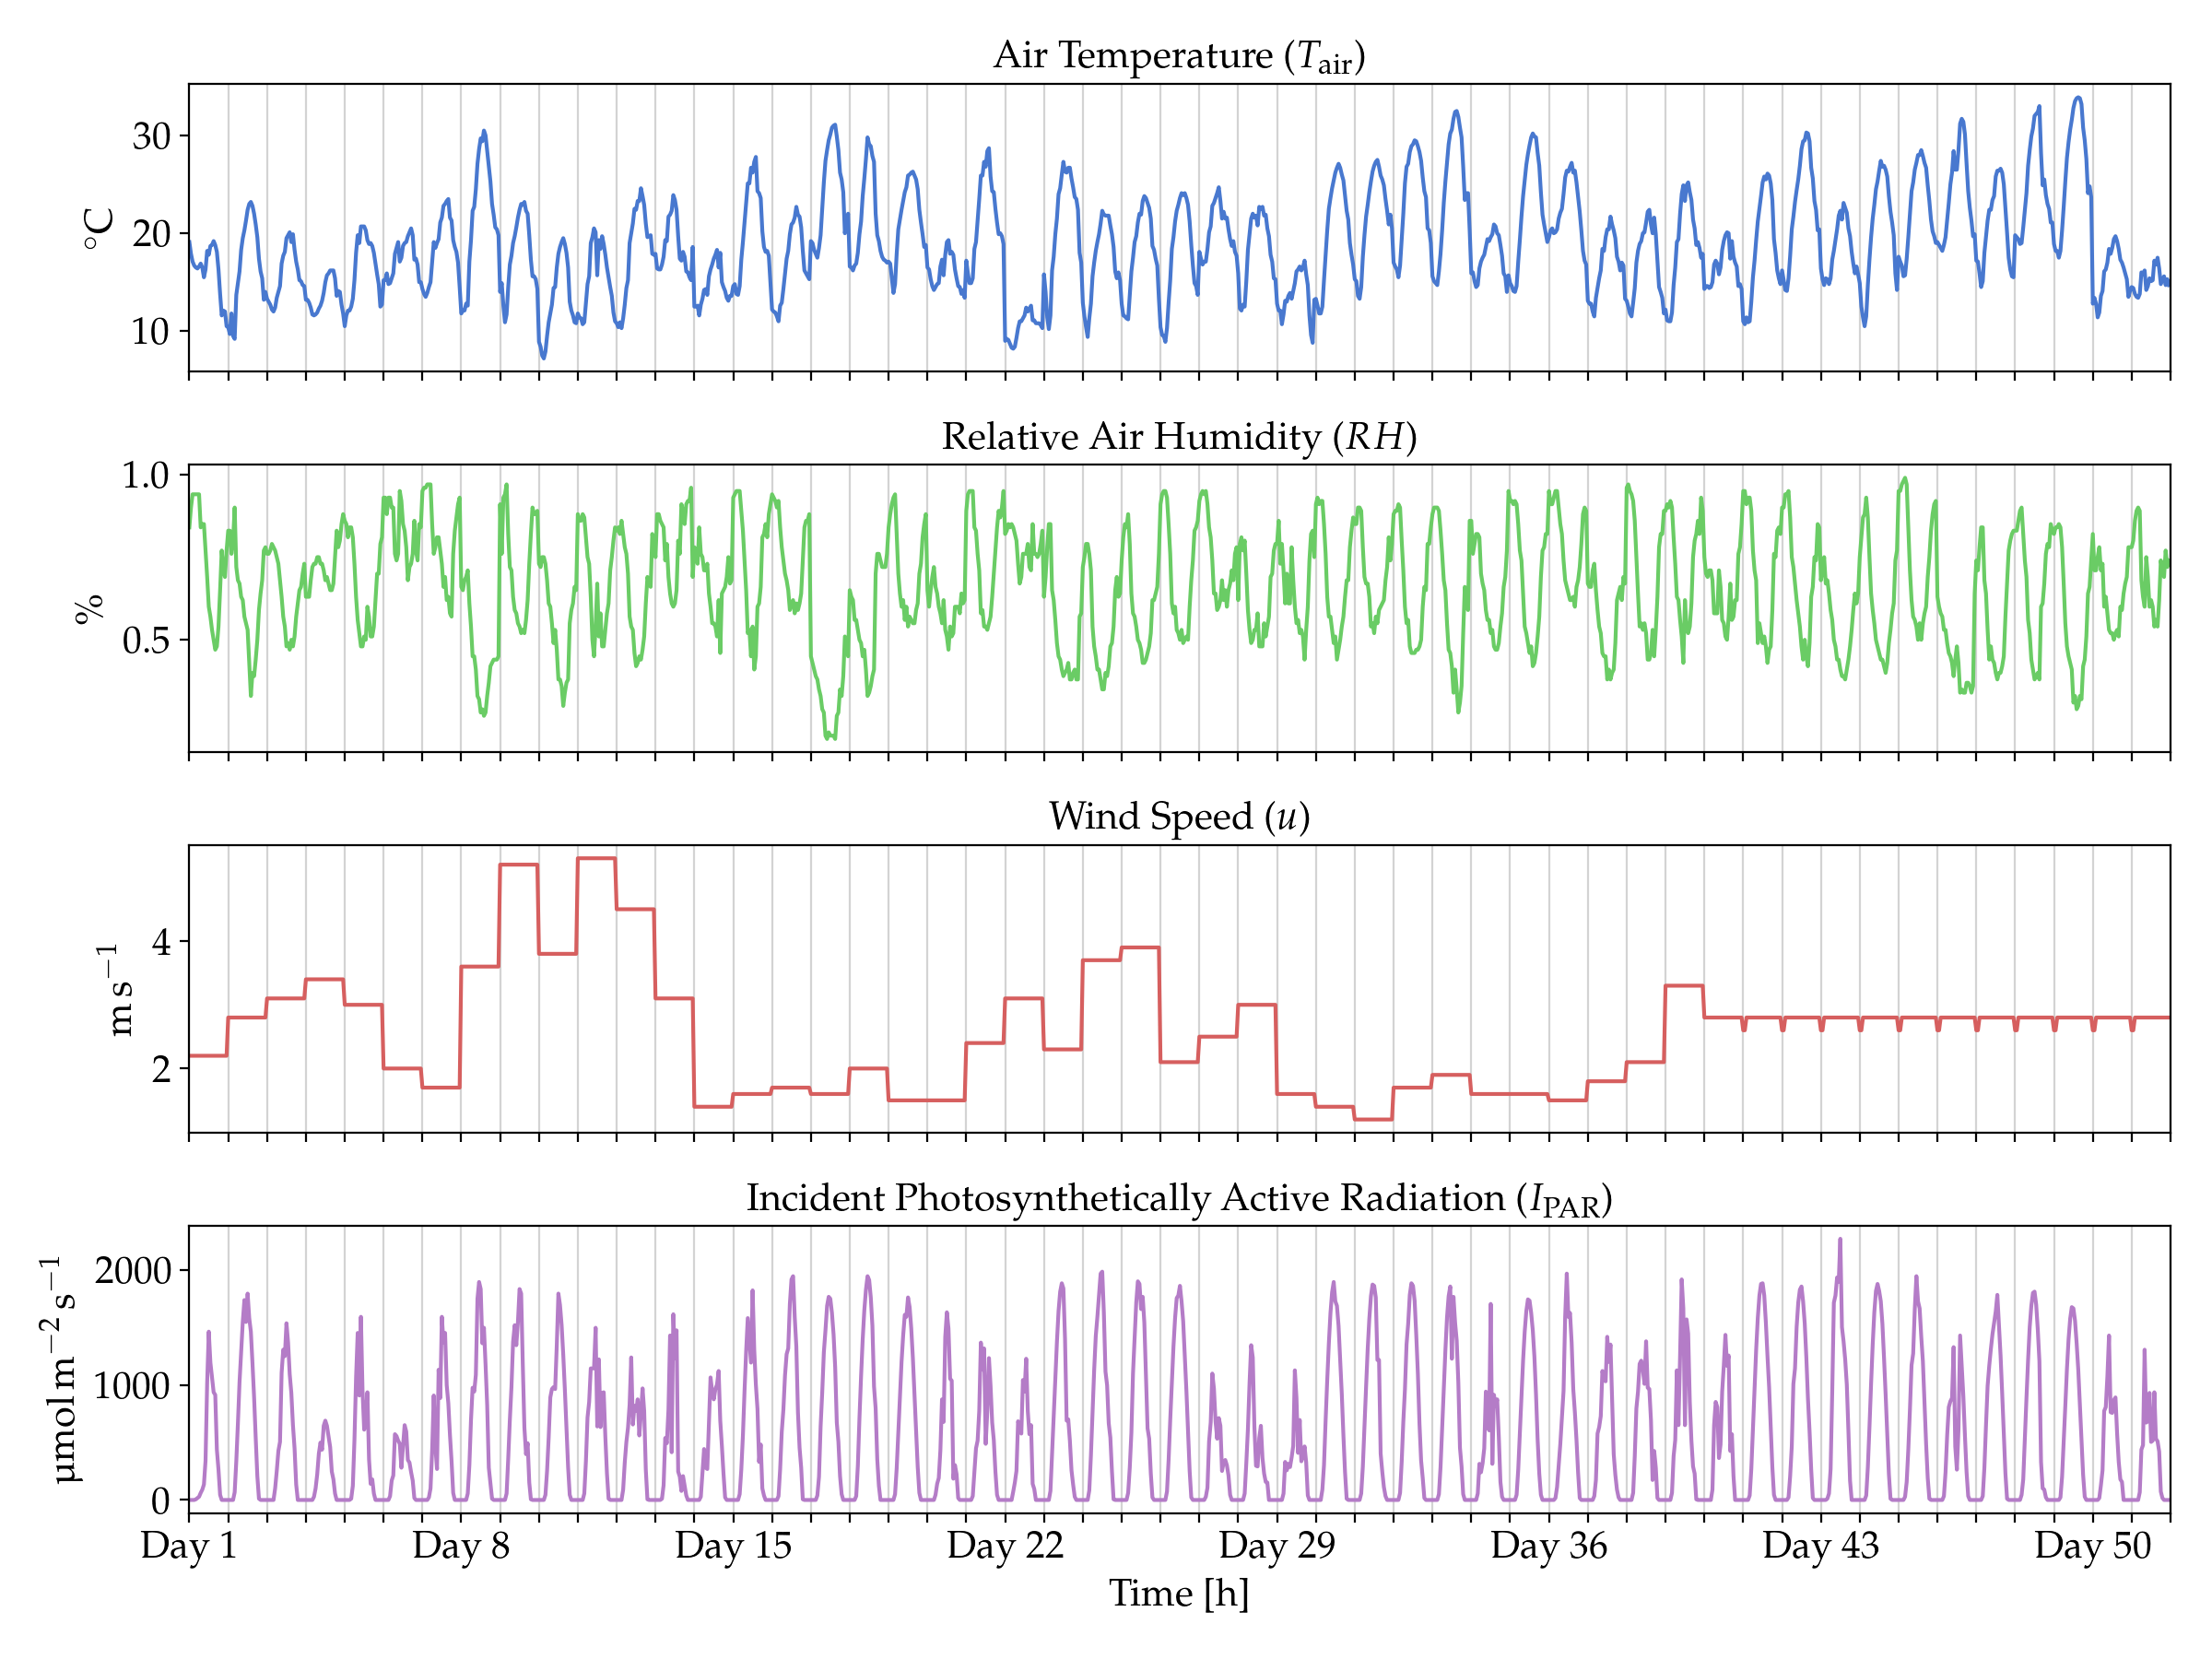
\includegraphics[width=\textwidth]{img/cn_inputs.png}
	\captionof{figure}[Hourly meteorological inputs used in CN-Wheat simulations.]
	    {
	    Hourly meteorological inputs used in CN-Wheat simulations.
	    The data was recorded in Clermont-Ferrand in central France. 
	    The data is a reconstruction of various dates in 2005.
	    See \citet{barillot_cn-wheat_2016-1} for more details.
    }
	\label{fig:cnwheat-meteo}
\end{minipage}}
% \end{sidewaysfigure}

\begin{sidewaysfigure}[ht]
	\centering
    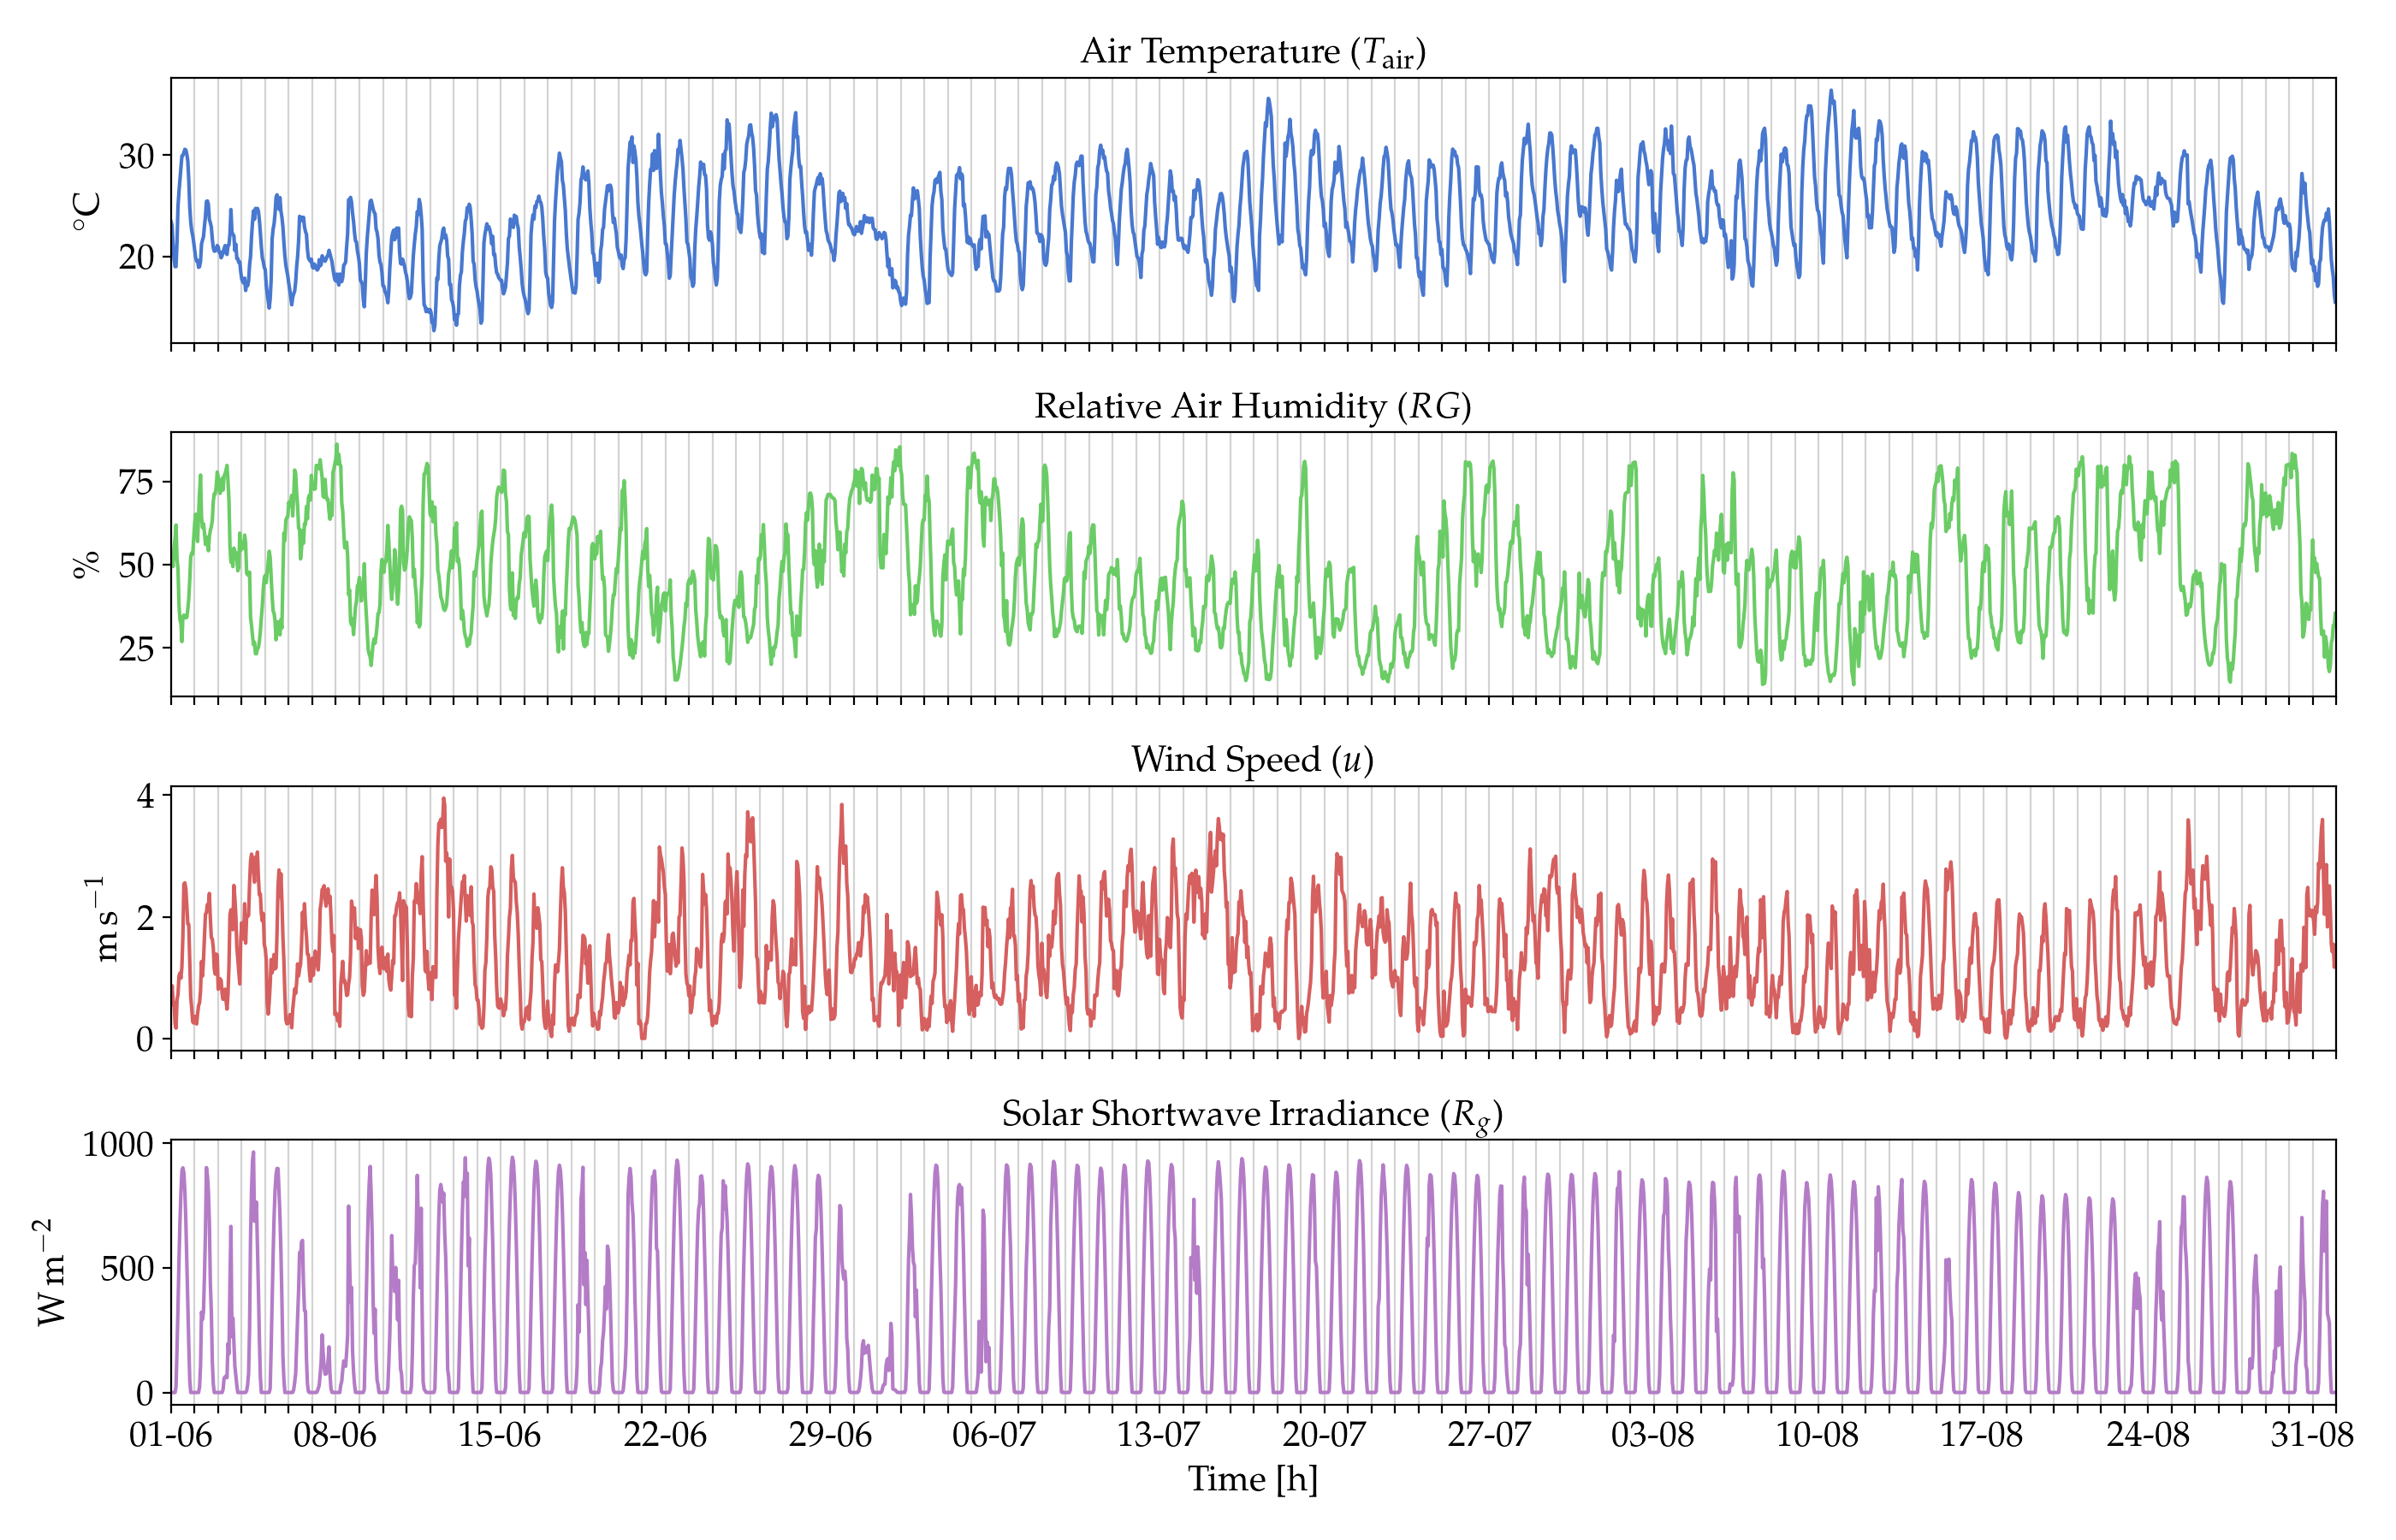
\includegraphics[width=\textwidth]{img/hs_inputs.png}
	\caption
	[Hourly meteorological inputs used in HydroShoot simulations.]
	{
	    Hourly meteorological inputs used in HydroShoot simulations.
	    The data originates from Montpellier, southern France and was recorded in 2012.
	    See \citet{albasha_hydroshoot_2019} for more details.
    }
	\label{fig:hydroshoot-meteo}
\end{sidewaysfigure}


\chapter{HydroShoot: Additional Information} \label{app:hydroshoot}

\section{Simulation Details} \label{app:hydroshoot-sim-details}

We used the ``GDC Canopy 1'' configuration from the public repository\footnote{The simulation code can be found at \url{https://github.com/openalea/hydroshoot}} in no water deficit mode.
We adapted the simulation duration to run longer than the four days in the original publication.
The model's first author, R. Albasha, communicated to us that the model had been used for simulation durations of up to a month.
However, the hydraulic model uses the soil water potential $\Psi_{\text{soil}}$ at the start of each day as input data.
Adding a realistic soil water model was out of scope for this work. We settled on a modest extension to seven days for regression experiments and ten days for the impulse experiment.
For this, we used a simple soil water model: we set $\Psi_{\text{soil}}$ input to a constant value of \SI{-0.40}{\mega\pascal} at the start of each simulation day.


\section{Reservoir Composition} \label{app:hydroshoot-reservoir}

We limited the reservoir to leaf elements only. 
Leaves are the least invasive to observe when transferring the experimental setup to an \textit{in vivo} scenario.
Besides, most processes from Table \ref{table:simulation_reservoirs} occur only in leaves.
Because the model structure includes 360 leaves, we randomly selected a subset of 32. 
The same random subset was used for all experiments.


\section{Regression Dataset} \label{app:hydroshoot-dataset}

We built the dataset from simulations using three months of input data (see Figure \ref{fig:hydroshoot-meteo}).
% We ran over eighty seven-day simulations to collect this data, with the simulation starts offset by one calendar day.
To collect this data, we ran more than eighty seven-day simulations, each started with an offset of one calendar day.
Figure \ref{fig:hydroshoot-grouping} illustrates how the overlapping simulation data was grouped for train, validation and test splitting.

% TODO: Figure showing grouping with simulation overlap


\section{Cross-Validation Strategy} \label{app:hydroshoot-validation}

Initially, we used the leave-one-group-out strategy as outlined in Section \ref{methods:validation}.
However, we noticed that the regularization parameter $\lambda$ has a smooth and relatively flat optimization landscape for this particular dataset. 
Because of this, we shifted to using a group-K-fold strategy with five folds.
The difference in model performance is negligible, but the speedup in optimization time is considerable.


\section{Setup Impulse Experiment} \label{app:hydroshoot-impulse}

For the impulse experiments, we used the same simulation configuration as described in \ref{app:hydroshoot-sim-details}.
We ran the simulations for ten days, starting at 2012-08-01.
We applied the impulse on midday of the fifth day. 
The model then ran for five more days.
We applied the stimulus to the incident solar irradiance (\acrshort{par}). We used values of 0 and 1500 \unit{\watt\per\meter\squared}. The latter corresponds to $\approx 1.6 \times$ the maximum amplitude of the natural signal.


\begin{figure}[]
	\centering
    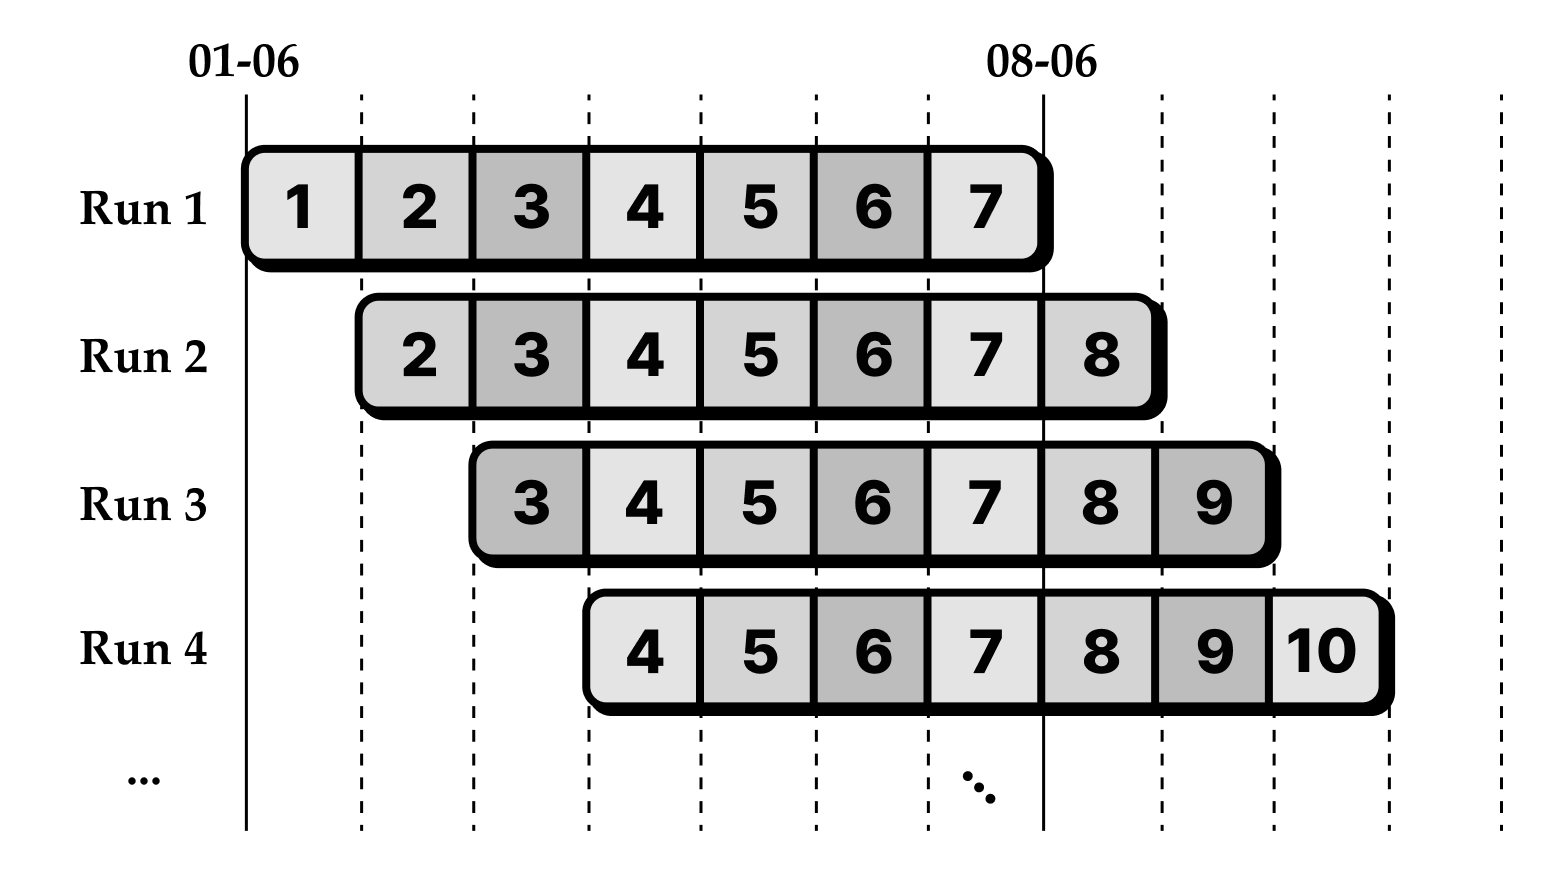
\includegraphics[width=11.65cm]{img/hs-grouping.png}
	\caption[Data grouping method used to combine data from overlapping simulation runs of HydroShoot.]{Data grouping method used to combine data from overlapping simulation runs of HydroShoot. Data with the same group number must stay together in a train, validation, or test set.}
	\label{fig:hydroshoot-grouping}
\end{figure}
\chapter{CN-Wheat: Additional Information} \label{app:cnwheat}

\section{Simulation Details} \label{app:cnwheat-simulation}

We used the post-vegetative simulations used for the ``NEMA'' experiment from \citet{barillot_cn-wheat_2016-1}\footnote{All simulations are available at \url{https://github.com/openalea-incubator/WheatFspm}}. 
We used the simulations for the H0, H3 and H15 fertilization regimes.
The simulations were run as-is for their entire fifty-day duration.


\section{Reservoir Composition} \label{app:cnwheat-reservoir}

In CN-Wheat, photosynthesis occurs in more than just the leaf elements.
Because the structural model is already small at just fifteen elements, we allowed all shoot elements to be part of the reservoir.
This left ten elements that track eco-physiological processes of interest (namely surface temperature $T_s$, transpiration rate $E$, stomatal conductance $g_s$, and net photosynthesis rate $A_n$).
However, we still selected a random sample of seven elements so that the readout model does not have total observability over the internal state of the plant model.


\section{Regression Dataset} \label{app:cnwheat-dataset}

We noticed in initial experiments that the reservoir dynamics have a sudden change at a specific time step in each simulation configuration (see Figure \ref{fig:cnwheat-regime-change}).
The time step is different for each of the fertilization regimes.
Because this regime change likely violates the assumption of a pseudo-static reservoir, we trimmed the output data to only include data from before the regime change.
After trimming, 29, 35, and 37 days of data from the H0, H3 and H15 simulations remain.

Because the same plant is used in all three scenarios, we combined the data into a single dataset; this gives us three different samples per time step.
Model scores trained on the combined dataset were comparable to or slightly lower than models trained using data from a single scenario.
But combining the datasets resulted in a lower variance in scores.
Figure \ref{fig:cnwheat-grouping} illustrates how the simulation data was grouped for train, validation and test splitting.

% TODO: Figure of regime change
% TODO: Figure of dataset grouping

\section{Cross-Validation Strategy} \label{app:cnwheat-validation}

We used the leave-one-group-out strategy from Section \ref{methods:validation} for finetuning the regularization parameter.

\section{Setup Impulse Experiment} \label{app:cnwheat-impulse}

The H3 simulation was used for all impulse experiments.
We applied the stimulus on day 19 of the meteorological inputs from Figure \ref{fig:cnwheat-meteo}. 
Each simulation ran its entire fifty-day course.
The impulse was applied to incident photosynthetically active radiation (\acrshort{par}).
We used amplitudes of 0 and 4000 \unit{\micro\mole\per\square\metre\per\second}. 
The latter corresponds to approximately twice the maximal naturally occurring signal strength. 

% \begin{figure}
%     \centering
%     \begin{subfigure}[b]{0.485\linewidth}
%         \centering
%         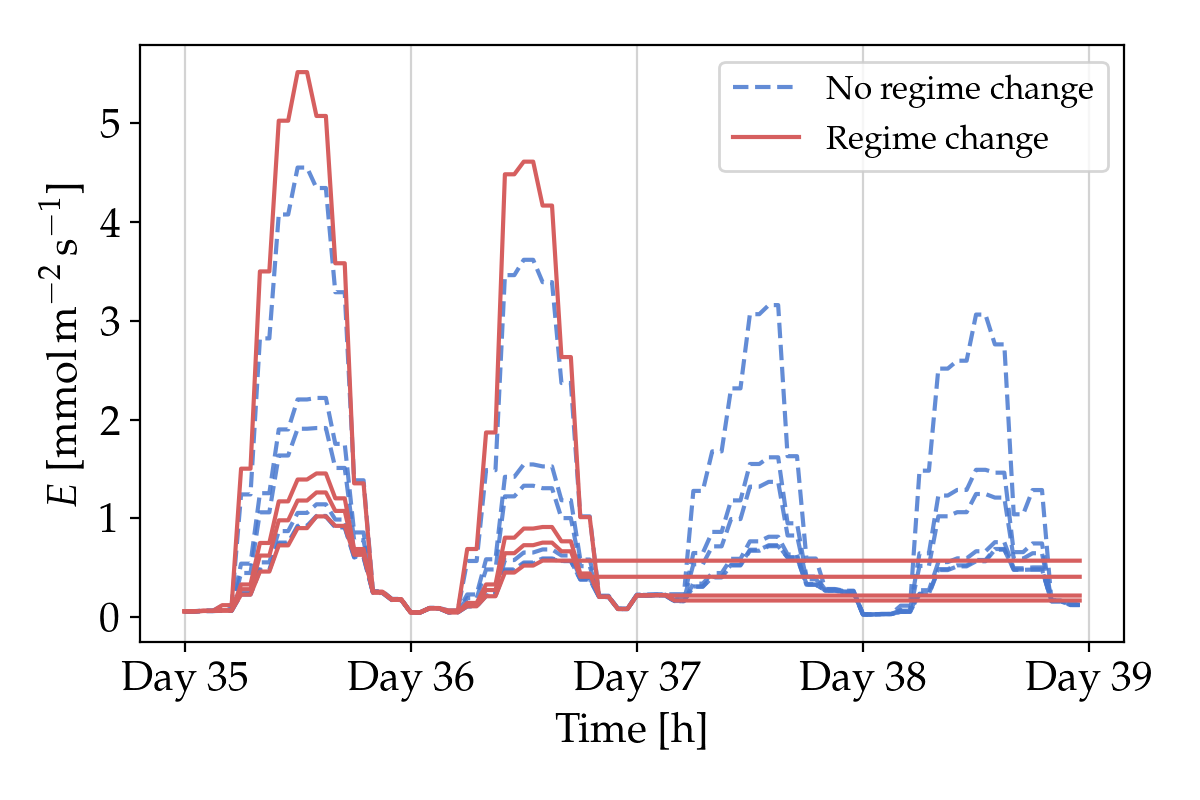
\includegraphics[width=\linewidth,height=\linewidth,keepaspectratio]{img/cn_regime_change.png}
%         \caption{HydroShoot}
%         \label{fig:hydroshoot-archi}
%     \end{subfigure}
%     \hfill
%     \begin{subfigure}[b]{0.485\linewidth}
%         \centering
%         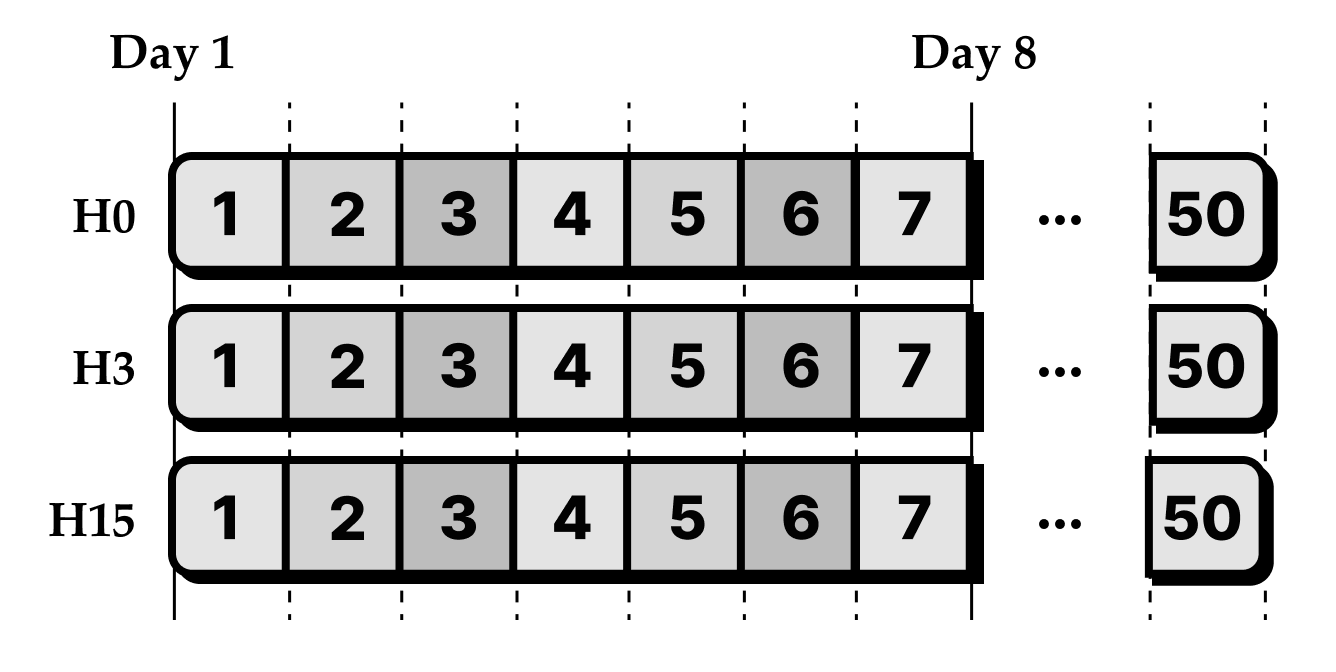
\includegraphics[width=\linewidth,height=0.85\linewidth,keepaspectratio]{img/cnw-grouping.png}
%         \caption{CN-Wheat}
%         \label{fig:cnwheat-archi}
%     \end{subfigure}
%     \caption{
%             FSPMs selected for use in experiments in this work. 
%             (\subref{fig:hydroshoot-archi}) A grapevine specimen from HydroShoot with the canopy trained in the ``Geneva Double Curtain'' configuration.  This figure is reused from \citet{albasha_hydroshoot_2019} under the CC BY 4.0 license.
%             (\subref{fig:cnwheat-archi}) The architecture of the CN-Wheat model. This figure is reused from \citet{barillot_cn-wheat_2016} with permission from the publisher (Copyright 2016 Oxford University Press).
%     }
%     \label{fig:appendix_cnwheat_figures}
% \end{figure}

\begin{figure}[]
	\centering
    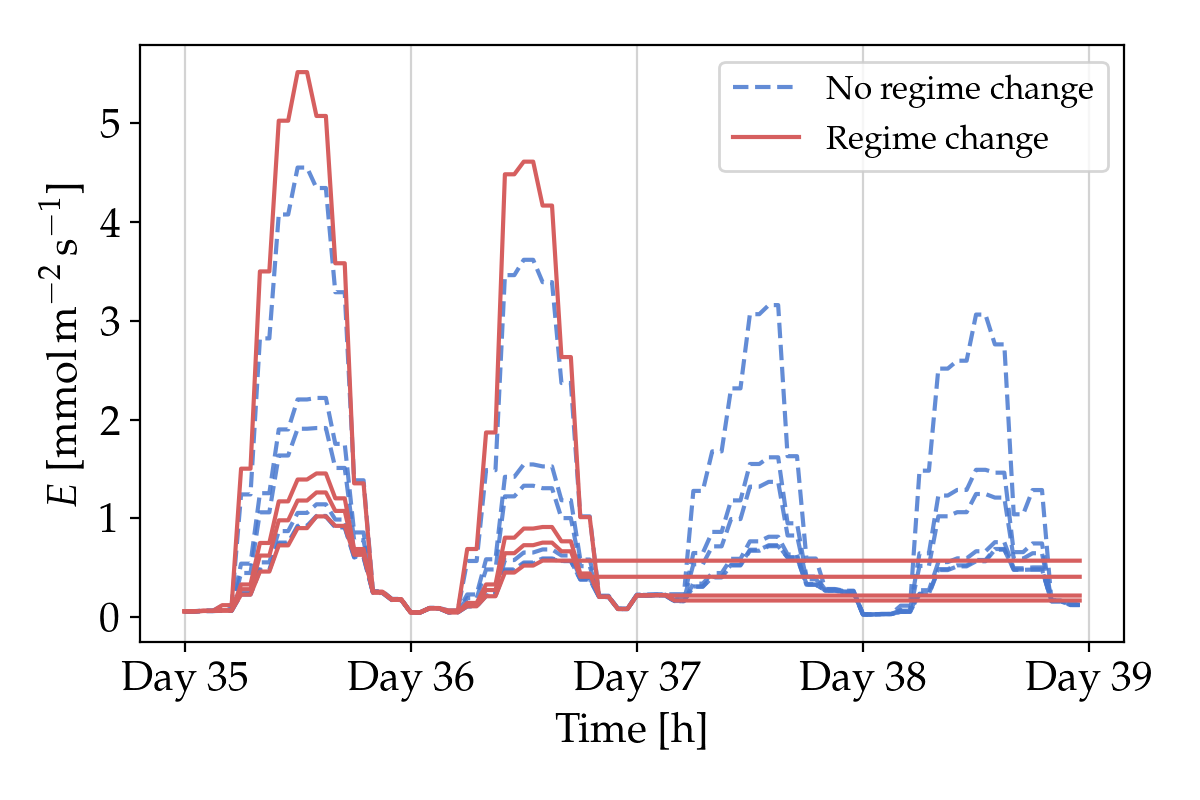
\includegraphics[width=10cm]{img/cn_regime_change.png}
	\caption[Some structural elements of CN-Wheat stop functioning after a specific amount of days.]{Some structural elements of CN-Wheat stop functioning after a specific amount of days. Depicted on the figure is the transpiration rate of each shoot element in the H3 simulation. The red elements change their behavior after day 37.}
	\label{fig:cnwheat-regime-change}
\end{figure}


\begin{figure}[]
	\centering
    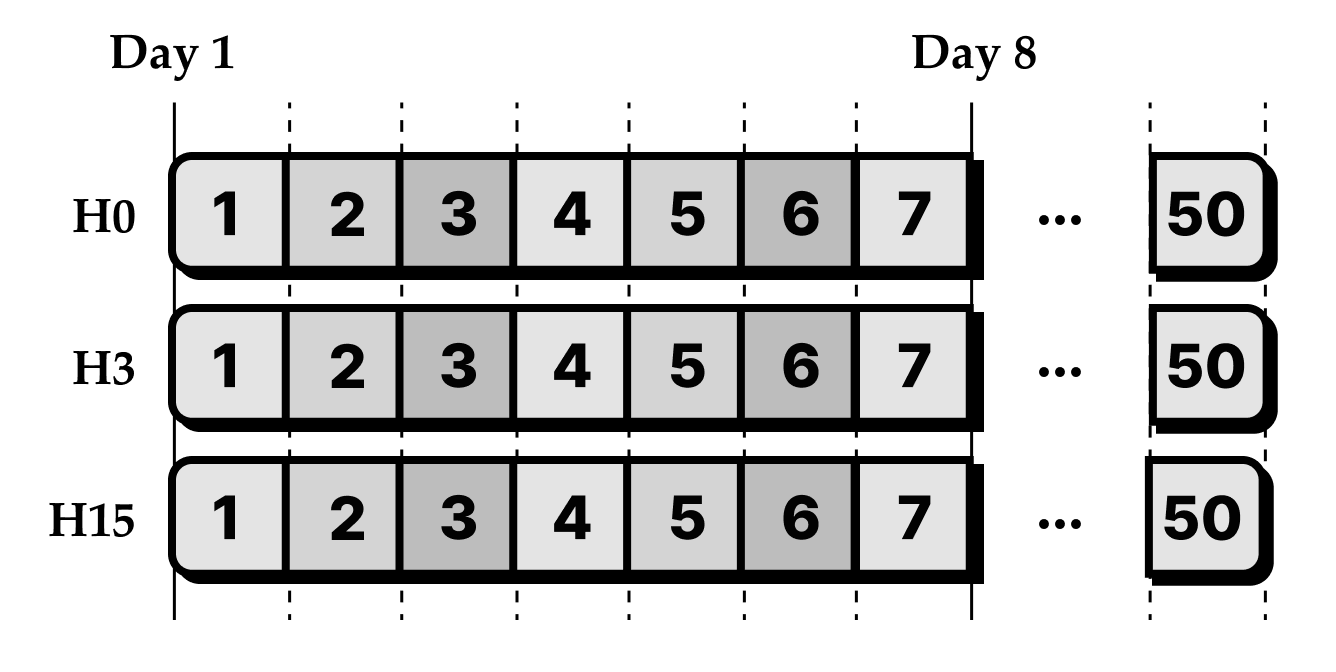
\includegraphics[width=10cm]{img/cnw-grouping.png}
	
	\caption[Data grouping method used to combine data from three simulations of CN-Wheat.]{Data grouping method used to combine data from three simulations of CN-Wheat. Data with the same group number must stay together in a train, validation, or test set.}
	\label{fig:cnwheat-grouping}
\end{figure}

% - Here we always used the H3 variant of the available simulations.
% - Impulse was applied on days X, Y, Z.
% - Impulse was never applied more than once per simulation run; avoided in case the impulse had a lasting effect on the reservoir.
% - We allowed the simulation to run its entire original course.
% - Impulse was applied to I_PAR, with value of 0, and 4000 mol/m2s (+-2x max amplitude in natural signal.)



\addcontentsline{toc}{chapter}{Bibliography}
\setlength\bibitemsep{1.5\itemsep}
\printbibliography


% mandatory closing pages
\newpage 
\fancyhf{} % Clear header/footer
\renewcommand{\headrulewidth}{0pt}
\pagenumbering{gobble}
\null
\newpage
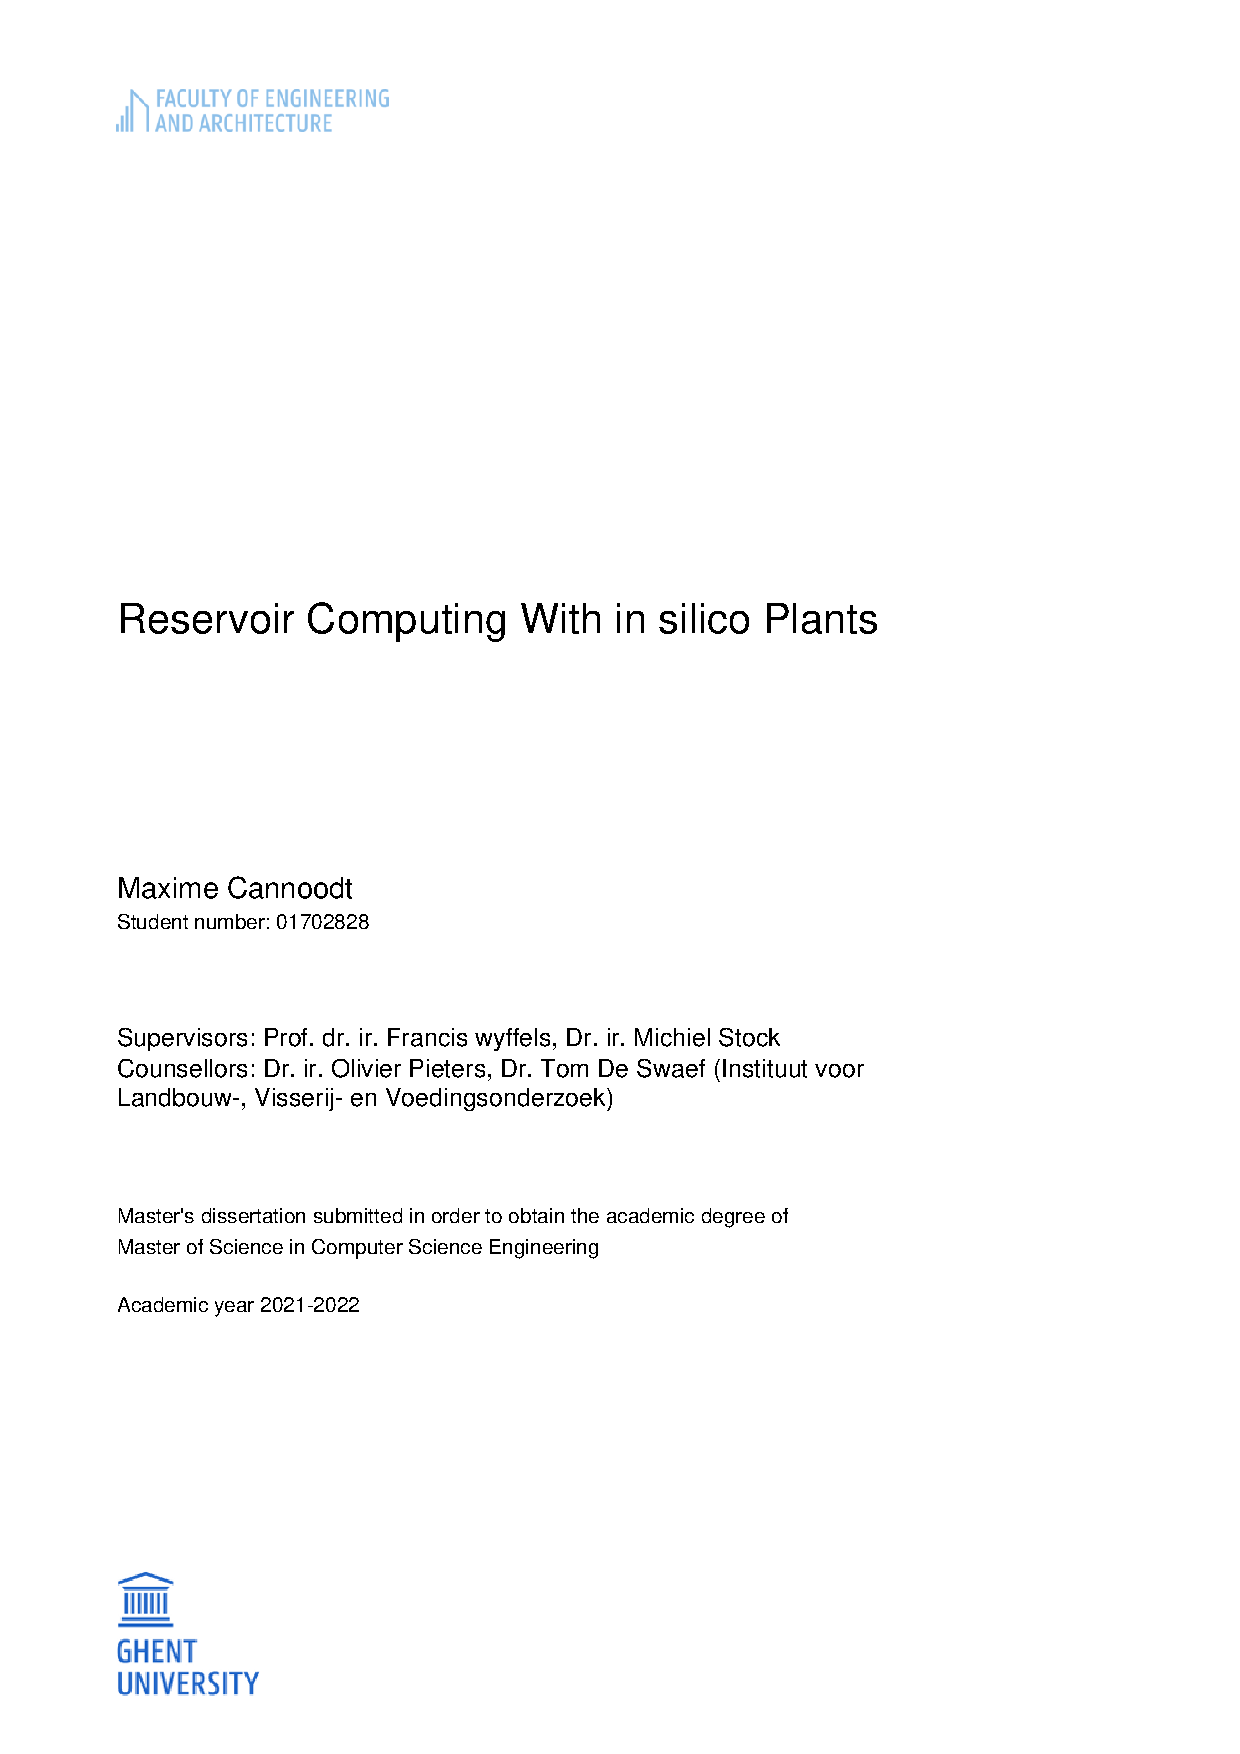
\includepdf[pages={1}]{cover-page-plato.pdf}

\end{document}
